% !TEX options=--shell-escape
\documentclass[oneside,openright,final,a4paper, oneside]{report}
\usepackage[top=3cm,bottom=3cm,inner=3.2cm,outer=3.2cm,symmetric,oneside]{geometry}
% \usepackage{fullpage}
% \usepackage[
%   margin=1.5cm,
%   includefoot,
%   footskip=30pt,
% ]{geometry}
% \usepackage{layout}

\usepackage{amsmath}
\DeclareMathOperator*{\argmax}{arg\,max}
\DeclareMathOperator*{\argmin}{arg\,min}

\usepackage{appendix}
% \BeforeBeginEnvironment{appendices}{\clearpage}

\usepackage{array}
\usepackage{graphicx}
\usepackage{multirow}

\newcommand\MyBox[2]{
  \fbox{\lower0.75cm
    \vbox to 1.7cm{\vfil
      \hbox to 1.7cm{\hfil\parbox{1.4cm}{#1\\#2}\hfil}
      \vfil}%
  }%
}

\usepackage{varioref}
\usepackage[hidelinks]{hyperref}
\usepackage[nameinlink, capitalise, noabbrev]{cleveref}


\newtheorem{hypothesis}{Hypothesis}
\newtheorem{nullhypothesis}{Null Hypothesis}
\usepackage{listings}
\usepackage{amsmath}

\usepackage[noline,ruled]{algorithm2e}
\setlength{\algomargin}{7.5pt}
\usepackage[utf8]{inputenc}
\usepackage[T1]{fontenc}
\usepackage{hyperref}
\usepackage{url}
\usepackage{booktabs}
\usepackage{amsfonts}
\usepackage{nicefrac}
\usepackage{microtype}

\usepackage{algorithmicx}
\usepackage{algpseudocode}
\usepackage{algorithm}
\usepackage{amsmath,amsthm}
\usepackage{xfrac}
\usepackage{multirow}
\usepackage{etoc}
\usepackage[titletoc,page]{appendix}
\usepackage{subfigure}
\usepackage{lipsum}



% \usepackage{listings}
\usepackage{minted}
\usemintedstyle{borland}
% \renewcommand{\lstlistingname}{Code}
\renewcommand\listingscaption{Code}
% \def\lstlistingautorefname{Alg.}


\usepackage{pgf,tikz}
\usepackage{mathrsfs}
\usetikzlibrary{arrows}

\newcommand{\bigCI}{\mathrel{\text{\scalebox{1.07}{$\perp\mkern-10mu\perp$}}}}



% theorem style
\RequirePackage{thmtools}

\RequirePackage{xcolor}


\definecolor{shadecolor}{gray}{0.95}


\usepackage{cleveref}

\crefname{listing}{code}{codes}
\Crefname{listing}{Code}{Codes}

\renewcommand{\aa}{\mathbf{a}}
\providecommand{\bb}{\mathbf{b}}
\providecommand{\cc}{\mathbf{c}}
\providecommand{\dd}{\mathbf{d}}
\providecommand{\ee}{\mathbf{e}}
\providecommand{\ff}{\mathbf{f}}
\let\ggg\gg
\renewcommand{\gg}{\mathbf{g}}
\providecommand{\hh}{\mathbf{h}}
\providecommand{\ii}{\mathbf{i}}
\providecommand{\jj}{\mathbf{j}}
\providecommand{\kk}{\mathbf{k}}
\let\lll\ll
\renewcommand{\ll}{\mathbf{l}}
\providecommand{\mm}{\mathbf{m}}
\providecommand{\nn}{\mathbf{n}}
\providecommand{\oo}{\mathbf{o}}
\providecommand{\pp}{\mathbf{p}}
\providecommand{\qq}{\mathbf{q}}
\providecommand{\rr}{\mathbf{r}}
\renewcommand{\ss}{\mathbf{s}}
\providecommand{\tt}{\mathbf{t}}
\providecommand{\uu}{\mathbf{u}}
\providecommand{\vv}{\mathbf{v}}
\providecommand{\ww}{\mathbf{w}}
\providecommand{\xx}{\mathbf{x}}
\providecommand{\yy}{\mathbf{y}}
\providecommand{\zz}{\mathbf{z}}
\providecommand{\aalpha}{\boldsymbol{\alpha}}
\providecommand{\ssigma}{\boldsymbol{\sigma}}
\providecommand{\llambda}{\boldsymbol{\lambda}}
\providecommand{\GGamma}{\boldsymbol{\Gamma}}


\providecommand{\mA}{\mathbf{A}}
\providecommand{\mB}{\mathbf{B}}
\providecommand{\mC}{\mathbf{C}}
\providecommand{\mD}{\mathbf{D}}
\providecommand{\mE}{\mathbf{E}}
\providecommand{\mF}{\mathbf{F}}
\providecommand{\mG}{\mathbf{G}}
\providecommand{\mH}{\mathbf{H}}
\providecommand{\mI}{\mathbf{I}}
\providecommand{\mJ}{\mathbf{J}}
\providecommand{\mK}{\mathbf{K}}
\providecommand{\mL}{\mathbf{L}}
\providecommand{\mM}{\mathbf{M}}
\providecommand{\mN}{\mathbf{N}}
\providecommand{\mO}{\mathbf{O}}
\providecommand{\mP}{\mathbf{P}}
\providecommand{\mQ}{\mathbf{Q}}
\providecommand{\mR}{\mathbf{R}}
\providecommand{\mS}{\mathbf{S}}
\providecommand{\mT}{\mathbf{T}}
\providecommand{\mU}{\mathbf{U}}
\providecommand{\mV}{\mathbf{V}}
\providecommand{\mW}{\mathbf{W}}
\providecommand{\mX}{\mathbf{X}}
\providecommand{\mY}{\mathbf{Y}}
\providecommand{\mZ}{\mathbf{Z}}
\providecommand{\mLambda}{\mathbf{\Lambda}}


\providecommand{\cA}{\mathcal{A}}
\providecommand{\cB}{\mathcal{B}}
\providecommand{\cC}{\mathcal{C}}
\providecommand{\cD}{\mathcal{D}}
\providecommand{\cE}{\mathcal{E}}
\providecommand{\cF}{\mathcal{F}}
\providecommand{\cG}{\mathcal{G}}
\providecommand{\cH}{\mathcal{H}}
\providecommand{\cI}{\mathcal{I}}
\providecommand{\cJ}{\mathcal{J}}
\providecommand{\cK}{\mathcal{K}}
\providecommand{\cL}{\mathcal{L}}
\providecommand{\cM}{\mathcal{M}}
\providecommand{\cN}{\mathcal{N}}
\providecommand{\cO}{\mathcal{O}}
\providecommand{\cP}{\mathcal{P}}
\providecommand{\cQ}{\mathcal{Q}}
\providecommand{\cR}{\mathcal{R}}
\providecommand{\cS}{\mathcal{S}}
\providecommand{\cT}{\mathcal{T}}
\providecommand{\cU}{\mathcal{U}}
\providecommand{\cV}{\mathcal{V}}
\providecommand{\cX}{\mathcal{X}}
\providecommand{\cY}{\mathcal{Y}}
\providecommand{\cW}{\mathcal{W}}
\providecommand{\cZ}{\mathcal{Z}}

\newcommand{\seb}[1]{}\newcommand{\sai}[1]{}\newcommand{\martin}[1]{}\newcommand{\jb}[1]{}

\usepackage{amsthm}
 
\theoremstyle{definition}
\newtheorem{definition}{Definition}[section]
 
\theoremstyle{remark}
\newtheorem*{remark}{Remark} 

\newcommand{\dataset}[1]{\emph{#1}}
\DeclareMathOperator{\topk}{top}
\DeclareMathOperator{\randk}{rand}
\newcommand{\R}{\mathbb{R}}
\newcommand{\abs}[1]{\left\lvert #1\right\rvert}
\newcommand{\norm}[1]{\left\lVert #1\right\rVert}
\DeclareMathOperator{\E}{\mathbb{E}}
\newcommand{\lin}[1]{\ensuremath \left\langle #1 \right\rangle}
\newcommand{\hogwild}{\textsc{Hogwild!}}

\usepackage[authoryear,square]{natbib}
\setlength{\bibsep}{5pt}
\date{}

\usepackage{pgf,tikz,pgfplots}
\pgfplotsset{compat=1.14}
\usepackage{mathrsfs}
\usetikzlibrary{arrows}

\definecolor{wwwwww}{rgb}{0.7,0.7,0.7}
\definecolor{bsqqqq}{rgb}{0.6980392156862745,0,0}
\definecolor{qqxycy}{rgb}{0,0.47058823529411764,0.7843137254901961}

\usepackage{titlesec}

\titleformat{\chapter}
  {\Large\bfseries} % format
  {}                % label
  {0pt}             % sep
  {\huge}           % before-code

\usepackage{enumitem}
\newcounter{impactcount}
\newlist{enumimpact}{description}{1}
\setlist[enumimpact,1]{%
  before={\setcounter{impactcount}{0}%
          \renewcommand*\theimpactcount{\arabic{impactcount}}},
        font={\bfseries\stepcounter{impactcount}I\theimpactcount~}
}
\newcounter{constraintcount}
\newlist{enumconstraint}{description}{1}
\setlist[enumconstraint,1]{%
  before={\setcounter{c}{0}%
          \renewcommand*\theconstraintcount{\arabic{constraintcount}}},
        font={\bfseries\stepcounter{constraintcount}C\theconstraintcount~}
}


\begin{document}

\begin{titlepage}
\begin{center}
%\large
\sffamily


\null
{\Huge Bayesian inference with Expectation \vspace{0.1cm}Maximisation for the characterisation of antibiotic treatment recovery in Cystic Fibrosis} \\[24pt]

\vspace{1cm}
{\huge Side project: Estimation of the variability in Cystic Fibrosis patient's FEV1 lung function measurements} \\[24pt]

\vfill

Master Thesis of \textbf{Tristan Trébaol}\\[9pt]
\vspace{1cm}

\begin{tabular} {cc}
\parbox{0.3\textwidth}{
\includegraphics[width=4cm]{images/logocam} \vspace{0.7cm}}
&
\parbox{0.7\textwidth}{%
University of Cambridge\\
  Department of Medecine\\[6pt]

Academic hosts\\[4pt]
%
    Prof. Andres Floto, Department of Medicine, University of Cambridge\\
    Ph.D. Damian Sutcliffe, Department of Medicine, University of Cambridge\\\\
    External Expert\\ John Winn, Machine Intelligence Group, Microsoft Research\\ [12pt]
}
\end{tabular}
\vspace{1cm}

\begin{tabular} {cc}
\parbox{0.3\textwidth}{
\includegraphics[width=4cm]{images/logoepfl} \vspace{4.1cm}}
&
\parbox{0.7\textwidth}{%
École Polytechnique Fédérale de Lausanne \\
  School of Engineering\\
  School of Computer and Communication Sciences\\[6pt]
%
Supervised by\\[4pt]
%
    Prof. Philippe Müllhaupt, School of Engineering, EPFL\\
    Prof. Martin Jaggi, Machine Learning and Optimization Laboratory, EPFL\\
    Dr. Mary-Anne Hartley, Machine Learning and Optimization Laboratory, EPFL \\\\\\\\ [12pt]
%
Cambridge, University of Cambridge, 2021}

\end{tabular}
\end{center}

\end{titlepage}






%\let\cleardoublepage\clearpage


% English abstract
\chapter*{Abstract}
% \markboth{Abstract}{Abstract}
\addcontentsline{toc}{chapter}{Abstract} % adds an entry to the table of contents

\textit{Main project.}\\
Chronic episodes of sudden pulmonary deterioration followed by insufficient recoveries from antibiotic treatments are the main driver of morbidity and mortality in Cystic Fibrosis (CF). Study of recovery is performed to improve CF care monitoring for those episodes. The characterisation of CF recovery with machine learning uses a data set of 119 antibiotic interventions from 55 patients. Patients, enrolled in a UK CF home monitoring study, recorded high dimensional physiological data daily, from which 8 bio-markers with a temporal resolution of 24 measurements per week are ingested. A multi-class Bayesian inference algorithm with convergence through expectation maximisation is formalised to successfully infer the characteristic profile of a typical recovery and of multiple types of recoveries. Further results based on those profiles suggest a prognosis for decline at recovery-end based on analysing the beginning of the post-treatment start behaviour. More importantly, the potential of machine learning to characterise recoveries is promising for future studies with additional longitudinal patient physiological data.\\\\
\textit{Side project.}\\
Forced Expiratory Volume in 1s (FEV1) is a key bio-marker to assess a CF patient lung health's status. However, its measurement is inherently subject to technical variability. Longitudinal high-frequency measurement data from the same UK CF home monitoring study can be used to redefine this variability. A bi-parameter moving average filter is built to segment signal and noise, the noise component of the model is analysed. The variability in FEV1 measurements is estimated to be 300mL with 21'000 lung function records from 220 patients. The variability is highly patient-specific (IQR [184; 428] mL), and not correlated with \%FEV1 predicted (r=0.129). Analysis of the impact of CFTR modulators shows that the start of Trikafta significantly mitigates the variability over any previous CFTR modulators history (6 homoscedasticity tests with p-value < 0.03), the same is not demonstrated for Symkevi.

\vskip0.5cm
\textbf{Key words}: cystic fibrosis, machine learning, statistics


% 

\cleardoublepage
\thispagestyle{empty}


\vspace*{3cm}

\begin{raggedleft}
    	If it were not for the great variability between individuals, medicine might as well be a science, not an art." \\ \hfill \break
     --- Sir William Oslen\\
\end{raggedleft}

\vspace{4cm}

I am thankful for Andres, Damian, John, and the University of Cambridge's Department of Medicine for hosting me for this master's thesis. I am particularly grateful for Damian for the excellent supervision, for sharing a thorough reviewing mindset and for accompanying me to explore different methods. In Switzerland, I am thankful for Philippe, Martin, and Annie, for their continuous support during my master's at EPFL, through our discussions and the many advice in the projects we undertook together. I am also highly grateful for the CF clinicians and researchers from Hôpital Necker Enfants Malades (France), Arizona Health Sciences Center (US) and Royal Papworth Hospital (UK), for providing an expert feedback on my work. Eventually, I would also like to thank all Project Breathe collaborators for building the richest CF data set of high-frequency physiological measurements in history. I trust that it will help to improve CFers lives condition even further than the current multiple benefits. More personally, as a CF patient and a researcher, it has been hard but also mind-opening to discover the diversity of CFers conditions. Studying CF in the spotlight of the life-changing Trikafta CFTR modulator therapy introduction in Europe was therefore particularly motivating.

\tableofcontents

\chapter{Introduction}

"If it were not for the great variability between individuals, medicine might as well be a science, not an art", Sir William Oslen, 1892. This statement still applies more than one century later, as clinicians still rely much on their personal and colleagues' experience to best treat patients, forming "mental models" for each disease. However, at the interface of biomedical signal processing, computational modelling, machine learning, and health informatics, computational healthcare turns medicine from art to science. From performing machine learning powered mechanistic studies, to communicating interpretable findings, computational healthcare can enable bespoke medicine, empower healthcare professionals, improve care pathways and public health policy, catalyse new therapeutics, and eventually improve population health.

Patients are complex due to their specific genetic backgrounds, medical histories, lifestyles, and distinct environmental exposure. This translates into different competing risks, variations in symptoms, distinct disease trajectories, and different responses to treatment. To address this, machine learning is promising as it can adapt the modelisation complexity to embrace patient variabilities. A comprehensive patient view can be built to provide interpretable analytics to clinicians. Deploying machine learning models in healthcare however needs to exploit a sufficient amount of data, taking the form of electronic health records, physiological time-series, genomics, and proteomics data. Diseases like Cystic Fibrosis (CF) that require continuous life-long monitoring can benefit the most from machine learning applications. Indeed, CF patients follow trimonthly clinics where many types of data are captured to generate the most adequate picture of the patient's health status \cite{gartner_2019}.

CF is the most common life-limiting genetic disorder in Caucasian populations that affects over 90,000 individuals worldwide \cite{bell_mall_2020}. It is caused by biallelic mutations in the Cystic Fibrosis Transmembrane conductance Regulator (CFTR) gene that, in the lung, lead to reduced airway surface liquid, impaired muco-ciliary clearance, chronic bacterial infections and, consequently, progressive inflammatory lung damage until premature death \cite{ratjen_bell_2015}\cite{elborn_2016}. Once considered as a pediatric disease, the majority of patients are now adults thanks to the remarkable advances in CF care improving life expectancy \cite{cff_registry_2019}. The most recent progress are CFTR modulators therapies that target the protein defect at the origin of the disease, thus greatly improving the airway microbiology \cite{rogers_2020}. Among them, the transformative triple therapy called Trikafta or Kaftrio is progressively being included as a regular treatment in the US since 2019, and in Europe since 2020.

Notwithstanding the promising progress on the path to cure CF, morbidity and mortality continue to be driven by episodes of sudden clinical deterioration, termed acute pulmonary exacerbations (APEs), from which patients do not recover fully. The succession of those episodes cause permanent loss of lung function \cite{sanders_2010}, impaired quality of life \cite{britto_2002}, and eventually premature death \cite{liou_2001}. Although the pathophysiology of, and the triggers for, APEs remain unclear, they are usually associated with: worsening symptoms of cough, breathlessness, and fatigue; increased volumes of purulent sputum; decreases in spirometry and sometimes oxygen saturations \cite{bilton_2011}. The lungs ineffectively recover due to a deficiency in the patients’ inflammatory response. Worse, the related dysregulation of the immune system participates in the patient's chronic inflammation status \cite{cantin_2015}, which requires external intervention including treatment with hospital or domiciliary antibiotics \cite{smith_2011}.

Given the importance of APEs and recovery on survival and wellbeing of individuals with CF, there is a critical need to better characterise the physiological changes preceding an APE and following a treatment. Whilst there has been an effort to characterise APEs, a focus on the recovery from antibiotic treatment is rare. Recent work analysed predictors for the onset of a successful recovery, but have been limited to a single feature (FEV1) and low temporal frequency (more than a month), in 2017 \cite{morgan_2017}\cite{sanders_2017}. They showed that patients do not return to 90\% of their baseline lung function in approximately 25\% of recoveries. However, questions such as "How does a recovery look like?, "Are there different types of recoveries?" remain unanswered. Since 2019, a large amount of multidimensional physiological data has been collected through two UK CF home monitoring studies, SMARTCARE and Project Breathe. They involved hundreds of patients self-reporting a dozen bio-markers on a daily basis \cite{damian}. The SMARTCARE data set proved to be rich enough to 1) characterise the typical profile of an APE, 2) infer different types of APEs, 3) predict their onset, using machine learning methods. Therefore it is wondered whether the study of APE could be complemented by the characterisation of the recovery after an antibiotic treatment, using the same machine learning methods.


% antibiotic resistance

\chapter{Background}  \label{sec:background}

\subsubsection{The Project Breathe study}
Project Breathe is an ongoing remote health home monitoring study for Cystic Fibrosis patients. It was created in 2019, by the UK Cystic Fibrosis Trust, the University of Cambridge, Royal Papworth Hospital, Magic Bullet, Microsoft, and Microsoft Research; perpetuating a successful previous 2-year feasibility study called SMARTCARE \cite{bach_2020}.

Patient’s individual data is collected on a daily basis through a free publicly available smartphone app, by using a Fitbit to track calories, sleep, and resting heart rate and weight via connected scales, an oximeter that measures blood oxygen levels, a spirometer that gauges lung function. That data is automatically uploaded to the app, and patients also enter self-reported information on how much they are coughing and how they’re feeling overall, as well as temperature. The complete list of measures is described in Table \ref{tab:measures}. Study data were link-anonymised and uploaded to a secure central server for collation and processing.

Project Breathe has two main purposes. Firstly, to allow patients to undertake a part of their follow-up remotely, through virtual clinics, where the data generated at home is automatically made available for the clinician in the hospital. This has multiple advantages. Patients 1) gain control over their health by also looking at the evolution of their measurements, 2) save time by not going to the hospital in person, and 3) have reduced risk of contracting nosocomial bacterial infections, as well as COVID-19. Hospitals patients' management is lightened and clinics can be programmed when they are really needed. By early 2020, Cardiff Hospital also started utilising Project Breathe. Two additional hospitals in the UK and a multi-site center in Canada are currently in the process of recruiting to Project Breathe.
Secondly, it provides multidimensional longitudinal CF patient data for CF research. Until now, half a million measurements were recorded, which makes it the richest available data set to study CF with such a high temporal frequency.

\subsubsection{Insight into the Project Breathe data at our disposal}
As program collaborators, access was granted to the participants from the Royal Papworth Hospital and Cardiff Hospital. It consists of 258 adults with CF, with characteristics broadly representative of the UK adult CF population \cite{uk_resigtry_2019}: mean age of 31.6 years, an average FEV1 of 69.0\% predicted, and 50\% homozygous for the CFTR F508del mutation (figure \ref{fig:breathestats}).
In addition, each study center was asked to provide clinical metadata for each participant including demographic details, sputum microbiology, and CFTR sequencing results; details and dates of hospital admissions and intravenous and oral antibiotic treatment courses and CFTR modulator therapy; and hospital-based measurement of lung function, weight, and C-reactive protein. Both home monitoring data and clinical metadata were then subjected to rigorous quality control (figure \ref{fig:dataqualitycheck}). Half of the individuals were given at least one antibiotic treatment during their enrollment time (figure \ref{fig:enrolmenttime}). This low amount can be explained by the introduction of effective CFTR modulators that are likely to mitigate the amount of APEs (table \ref{tab:cftrmodulators}), and by the short history for the recently enrolled participants (figure \ref{fig:nintr}). Compared to conventional clinical measurements, that are limited to periods when patients attend hospital (figure \ref{fig:clinic}), home monitoring provides an extremely rich dataset (figure \ref{fig:home}) with clear changes in signals in the period following the start of antibiotic treatment, supporting our attempt to characterise recovery with such data.

\subsubsection{Related work: characterisation of APEs}
Recoveries are preceded by APEs. Depending on the type of the decline (e.g. full decline, partial decline, no decline), the recovery is likely to behave differently. Sutcliffe et al. analysed APEs using data from the SMARTCARE study \cite{damian}. They studied 8 features, namely cough, wellness, FEV1, O2 saturation, activity in number of steps, pulse rate, and sleep from 104 adult patients. The main differences between SMARTCARE and Project Breathe are that the first was 2-year time-bounded with patients from seven centers required to record data for at least 6 months while the second is ongoing since 2019 with one center, extended to three others. With a long-term mindset, participants of Project Breathe were slightly less committed to the recording of measurements but provided more data.

The aim was triple: 1) validate that multimodal physiological data contained a signal that could be used as a proxy for the patient's health status, 2) define the profile of an APEs, and 3) predict the onset of APEs. The first goal was validated by successful results for the others. This work's focus is on point 2): they created a probabilistic inference machine learning model, using a Bayesian approach and with convergence through expectation maximisation, that was able to align APEs profiles on the exacerbation start, the onset of the decline in the different features. This was used to draw the typical profile of an APE and to infer multiple types of exacerbations, where three main classes were found. It was decided to mirror this study by characterising recoveries utilising the same machine learning model with requested adaptation and improvements. The next chapter details the project's aim and objectives.

\chapter{Aim \& Objectives}
% \addcontentsline{toc}{chapter}{Aims \& Objectives}
\label{sec:obj}

\subsubsection{Main project}
This thesis aims to improve CF care management by the characterisation of recovery after antibiotic treatment. This subject was approached with the following mindset: ask clinical questions to the data, answer them with machine learning and statistical methods, and eventually precise the results through feedback from the clinicians. The 5 objectives were:

\begin{enumerate}
    \item Review the literature of CF recovery after a treatment
    \item Develop an expert eye to extracting recovery information through analysing patients' multivariate longitudinal data
    \item Understand adapt the machine learning model for Bayesian inference with expectation maximisation, eventually update it where necessary and optimise its core parameters
    \item Infer the profile of a typical recovery from antibiotic treatment
    \item Investigate if multiple types of recoveries can be inferred using the algorithm
\end{enumerate}

\subsubsection{Side project}
A side project was performed to estimate the variability in forced expiratory volume in 1s (FEV1) measurements. This was initially requested for other research projects in the Department of Medicine. However, the model could demonstrate the impact, or the absence of impact, of  CFTR modulators therapies, mainly Symkevi and Trikafta on the variability. This was done during the two first months of the thesis as part of the introduction to Project Breathe's data and in parallel with the recovery work. It is described in section \ref{sec:sideproject}. The 4 objectives were:
\begin{enumerate}
    \item Review the literature of FEV1 variability estimation
    \item Build a model to estimate the variability in FEV1 measurements
    \item Review the literature for hypothesis testing methods to test homoscedasticity, i.e. equality of variance.
    \item Use the model to demonstrate the effect of CFTR modulators and distinguish patients with similar lung health
\end{enumerate}

\chapter{Material and Methods: the alignment model} \label{sec:model}
This chapter contains the material and methods necessary to understand the mathematical model used for the recovery study. The majority of the content concerns Bayesian inference, which confers a probabilistic approach to infer to learn the typical recovery curve and classify different types of recoveries. 

\section{Description} 
\subsection{Concept} 
The alignment model's objective is to draw the typical profile of a recovery. Looking at figure \ref{fig:schematics}, since patients start antibiotic treatments in different conditions, the raw patient data is unusable. However, patterns in the behaviour can be observed by aligning the antibiotic interventions to one another and averaging their values. The alignment model was used to 1) infer the profile of recovery for each type of measure, and 2) learn the recovery start date as an offset from the treatment starts for each data record.

    \begin{figure}[!h]
    \caption{Alignment model schematics}
    \centering
    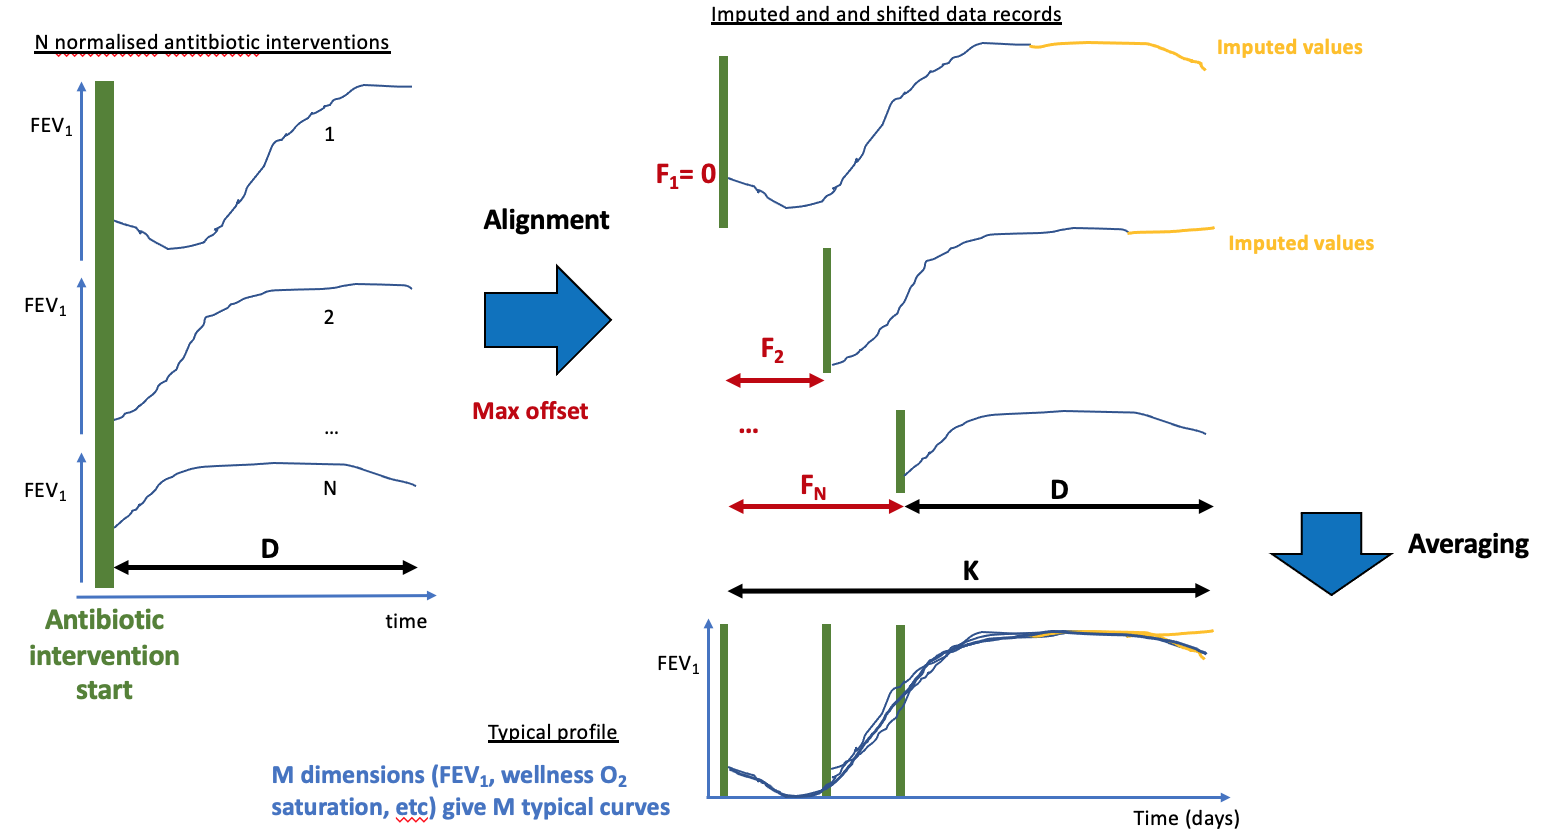
\includegraphics[width=150mm]{images/schematics.png}
    \label{fig:schematics}
    \end{figure}

\subsection{Reasons for the model}
Sutcliffe et al. \cite{damian} addressed the issue of curve alignment in their study of APEs. They proved that a probabilistic inference algorithm could learn the typical profile of an APE despite the scarcity, the noisiness, the presence of abrupt changes in the data.

The recovery analysis uses this algorithm written in MatLab. The rest of the section dives into the description and the mathematical formulation of this model. Note that it was decided to include the terminology related to the recovery to improve clarity and avoid repetitions.

\subsection{Terminology} \label{sec:datainputs}
To begin with, three main model concepts can be described:

\subsubsection{Data record}A data record, also called an (antibiotic) intervention, is a data sample of length D containing the set of home measurements performed during the period immediately following antibiotic treatment. A data record contains M times-series of the physiological data for each selected measure among the measures list introduced in table \ref{tab:measures} (FEV1, $O_2$ Saturation, Cough, Wellness, etc). The data records are $\mu$-normalised based on the patient's last stable values, this allows to easily observe full recoveries when signals come back to the stable baseline, and $\sigma$-normalised by the patient measure's mean amplitude, to harmonise data records across patients.

\subsubsection{Typical profile}The typical profile, or latent curve, of length K is the superposition of all data records, shifted by the optimal allowed offsets. The typical profile is thus longer than the data record by several days equal to the span of the offsets.

\subsubsection{Offsets}The offset values are the number of days by which a data record is allowed to be shifted upwards from the treatment start. There are exactly K-D offsets. Offset values are defined as follows. 1) for an offset of 0 the recovery starts at the same time as the announced treatment. The data record is not shifted. 2) For positive offsets the data record is shifted upwards, further away from the recovery start.

\subsubsection{Important notes:}
\begin{enumerate}
    \item The offset range is [1,K-D], but since the minimum offset is 0, for which the position of the data record is not changed, the offset values range is [0,K-D-1]. 
    \item As the data record is D-day long and the typical profile is K-day long, there are always K-D slots on the typical profile to which the data record is not contributing. Indeed, when the data record is shifted by an offset of $f$ to the right of the typical profile, the data record is solely contributing to [1+$f$;$f$+D] points on the typical profile.  
\end{enumerate}

\section{Mathematical formulation}

\subsection{Definition of the generative process} \label{sec:datagen}
The generative model creates the foundation of the inference algorithm. The machine learning model and associated variables can be represented as a factor graph (figure \ref{fig:graph}). There is one observed point – the measured value (V) - for each data record (N), for each day in the data record (D), and each type of measure (M). It was assumed that the measured value arises from the corresponding point on the typical profile for measure M, plus some Gaussian noise. Each day in a typical profile is made up of a mean value ($Z_{m,k}$), and a standard deviation from the mean ($S_{m,k}$) used to define the amount of noise added. Each typical profile can be up to K days long, K > D, where there is a pair of values of $Z_{m,k}$ and $S_{m,k}$ for each day. For each data record, there is also a latent variable for the offset ($F_n$) which is used to compare the data record to different places of the typical profile, to allow the recovery start inference. This takes the form of a probability distribution over the allowed (K-D) number of offsets.

    \begin{figure}[!h]
    \caption{Interventions by duration}
    \centering
    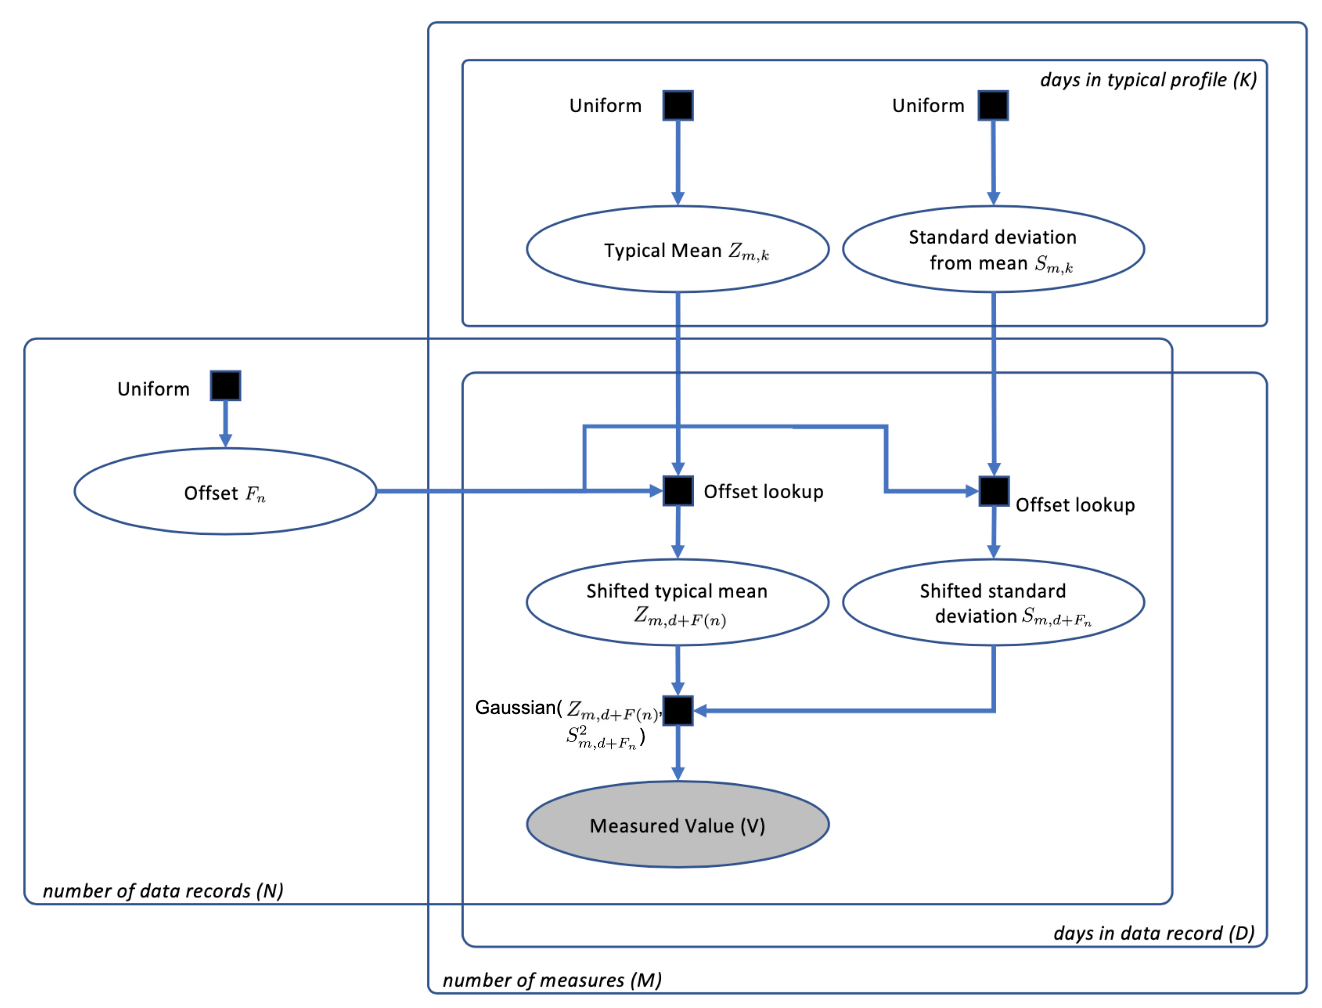
\includegraphics[width=130mm]{images/factorgraph.png}
    \label{fig:graph}
    \end{figure}
    
\begin{algorithm}[H]
\For{\mbox{each measure m = 1 to M}}{
    \For{\mbox{each day in the typical profile k:=1 to K}}{
        Draw a typical value $Z_{m,k}$ from an improper uniform distribution over $\mathbb{R}$\\
        Draw a noise standard deviation $S_{m,k}$ from an improper uniform distribution over $\mathbb{R^{+}}$
        }
    }
\For{\mbox{each data record n = 1 to N}}{
    Pick an offset $F_{n}$ from a uniform distribution $\mathcal{U}$(0,K-D-1)\\
    \For{\mbox{each day in the data record  d:=1 to D}}{
        \For{\mbox{each measure  m:=1 to M}}{
            Draw a typical value $Z_{m,k}$ from an improper uniform distribution over $\mathbb{R}$\\
            Generate a (normalised) measured value $V_{n,m,d}$ from the random variable $\mathcal{V}_{m,d+F_n}$ following a normal distribution of such that: such that $\mathcal{V}_{m,d+F_n} \sim \mathcal{N}(Z_{m,d+F(n)}, S_{m,d+F(n)}^2)$
            }
        }
    }
 \caption{Generative process}
\end{algorithm}

Note: prior to observing the data the values of $Z_{m,k}$ and $S_{m,k}$ are completely unknown. $Z_{m,k}$ could be set to any real value and $S_{m,k}$ to any real positive value. Hence, the prior probability distribution for $Z_{m,k}$ and $S_{m,k}$ have to be set to improper distributions.

\subsubsection{Sampling interpretation} 
Running this process samples from the joint distribution P($Z_{m,k}$, $F_n$, $V_{n,m,d}$). The data set is generated by repeatedly sampling values and filtering the ones that actually correspond to measured values. Eventually, this gives samples from P($Z_{m,k}$, $F_n$ | $V_{n,m,d}$).

\subsubsection{This generative process makes three assumptions:}
\begin{enumerate}
    \item For each measure, the recorded values for the period immediately following treatment are a noisy version of a single typical profile.
    \item The amount a measured value deviates from this profile is controlled by the position on the profile and is independent from one day to the next.
    \item The treatment start can happen anytime between day 1 and the maximum allowed offset (K-D).
\end{enumerate}

\subsection{Probabilistic inference algorithm}
Since the offset of each data record is unknown, the true value of the pairs ($Z_{m,k}$ and $S_{m,k}$) cannot be derived analytically. Given the available data, the objective of the inference algorithm is to reconstruct a trustworthy image of each measure's typical profile by interpolating the calculated estimates $Z_{m,k}$, $S_{m,k}$. Expectation maximisation (EM) \cite{neal_1998} \cite{billard_2018} is used to infer the data record offset probability distribution $F_n$ and compute the estimates. The EM algorithm alternately computes:
\begin{enumerate}
    \item \textbf{E-step:} The expectation of the distribution over each offset F, with Z and S fixed. This updates the probability distribution of offsets for each data record.
    \begin{equation}\label{eq:obj}
    \forall n \in [1;N], Obj_n = = -\frac{1}{2} \cdot \sum_{m=1}^M \sum_{d=1}^D \left[ A + \left( \frac{V_{n,m,d} - Z_{m,d+F_n} + B}{ S_{m,d+F_n} } \right)^2 \right],
\end{equation} 
with
\begin{equation}
    A = \ln(2\cdot \pi) + 2\cdot \ln( S_{m,d+F_n} )
\end{equation}
\begin{equation}
    B = 
    \begin{cases}
        \min (\alpha, \overline{V}_{n,m} - \overline{Z}_{m,F_n} ), & \text{for } \overline{V}_{n,m} - \overline{Z}_{m,F_n} \geq 0\\
        \max (-\alpha, \overline{V}_{n,m} - \overline{Z}_{m,F_n} ), & \text{for } \overline{V}_{n,m} - \overline{Z}_{m,F_n} < 0
    \end{cases}
\end{equation}
    \item \textbf{M-Step:} Each point in the latent profile is updated to the new maximum likelihood estimator, with the offset probability distribution fixed. This updates the typical profile.
\begin{equation}
    \forall k \in [1;K], m \in [1;M],
    \begin{cases}
        Z_{m,k}' = \frac{ \sum_{n=1}^N \sum_{f=0}^{K-D-1} V_{n,m,k-f} \cdot P(f) \cdot W(k,f) }{ \sum_{f=0}^{K-D-1} P(f)\cdot W(k,f) }\\\\
        S_{m,k}' = \frac{\left( \sum_{n=1}^N \sum_{f=0}^{K-D-1} V_{n,m,k-f} \cdot P(f) \cdot W(k,f) \right)^2}{ \sum_{f=0}^{K-D-1} P(f)\cdot W(k,f) } - Z_{m,k}^{'2}
    \end{cases}
\end{equation}
with
\begin{equation}
    W(k,f) = 
    \begin{cases}
        1, & \text{for } k > f\\
        0, & \text{for } k \leq f\\
    \end{cases}
\end{equation}
\end{enumerate}

\subsubsection{Initialisation and end-state}
The model initialisation is as follows: for each measure and data record, the probability distribution of the offsets $P(F_n)$ is uniformly distributed over the span of allowed offsets. The algorithm then starts with an M-step, and sequentially computes expectation and maximisation steps until convergence.

After convergence, the end-state of the inference algorithm is a mapping $\mathcal{F}$, defined below, that places the data record on the typical profile at the most probable offset location. A last maximisation step with $\mathcal{F}$ is performed to obtain the $Z_{m,k}$, $S_{m,k}$ of the final profile through point estimation for each offset, rather than the previously used offset probabilistic estimation. $\mathcal{F}$ has thus the $N \times K-D$ possibilities.
\begin{equation}
    \mathcal{F} : [1;N] \longrightarrow [0;K-D-1],  n \longmapsto F_n, F_n = \argmax_{[1;K-D]}(P(F_n)))-1
\end{equation}
\textit{The objective of the algorithm is to find $\mathcal{F}$ that minimises the squared sum of distances between each shifted data record and the typical profile.}

\subsubsection{Derivation of the E-step}
For each data record n, given the set of measured values $V_n$, and the set of parameters Z and S fixed from the previous M-step, one can compute the posterior distribution according to Bayes theorem \cite{olhede_2018}:

\begin{equation}
    P(F_n|V_n,Z,S) = \frac{P(V_n|F_n,Z,S) \cdot P(F_n)}{P(V_n,Z,S)}
\end{equation}
Since the prior distribution for the offsets is uniform, and $P(V_n,Z,S)$ is fixed,
\begin{equation}
    P(F_n|V_n,Z,S) \propto P(V_n|F_n,Z,S)
\end{equation}
The total probability of observing the set $V_n$ given $F_n$, Z, and S fixed is the likelihood function. As it was assumed that the measured values from the set $V_n$ are identically and independently distributed, the likelihood function is the product of the  probability distributions of the random variables $\mathcal{V}_n$ from which they are drawn. Hence the probability distribution for the offsets writes:
\begin{equation}
    P(F_n|V_n,Z,S) = \prod_{m=1}^M \prod_{d=1}^D P(V_{n,m,d}|F_n,Z_{m,d+F_n},S_{m,d+F_n})
\end{equation}
\begin{equation}
    P(F_n|V_n,Z,S) = \prod_{m=1}^M \prod_{d=1}^D \frac{1}{ \sqrt{2\cdot\pi\cdot S_{m,d+F_n}^2} } \cdot exp \left[ -\frac{1}{2} \cdot \left(\frac{V_{n,m,d} - Z_{m,d+F_n}}{ S_{m,d+F_n} }\right)^2 \right]
\end{equation}
In the log space, the objective function $Obj_n$ is obtained by computing the error between the shifted data record measures' time-series and the typical profile:
\begin{equation}
    \forall n \in [1;N], Obj_n = \ln(P(F_n|V_n,Z,S)) = -\frac{1}{2} \cdot \sum_{m=1}^M \sum_{d=1}^D \left[ A + \left( \frac{V_{n,m,d} - Z_{m,d+F_n}}{ S_{m,d+F_n} } \right)^2 \right],
\end{equation} 
with $ A = \ln(2\cdot \pi) + 2\cdot \ln( S_{m,d+F_n} )$

\subsubsection{Derivation of the M-step}
Given the offsets probability distribution $P(F_n)$, Z and S are updated to Z' and S' via maximum likelihood optimization. 
\begin{equation}
    \begin{cases}
        Z' = \argmax_Z(P(F_n|Z,V_n)) \\
        S' = \argmax_S(P(F_n|S,V_n))\\
        % note how to calculate the likelihood function?
    \end{cases}
\end{equation}

It corresponds to a variation of the maximum likelihood estimator for the normal distribution calculated for each offset and weighted by the probability distribution of the current offset:
\begin{equation}
    \forall k \in [1;K], m \in [1;M],
    \begin{cases}
        Z_{m,k}' = \frac{ \sum_{n=1}^N \sum_{f=0}^{K-D-1} V_{n,m,k-f} \cdot P(f) \cdot W(k,f) }{ \sum_{f=0}^{K-D-1} P(f)\cdot W(k,f) }\\\\
        S_{m,k}' = \frac{\left( \sum_{n=1}^N \sum_{f=0}^{K-D-1} V_{n,m,k-f} \cdot P(f) \cdot W(k,f) \right)^2}{ \sum_{f=0}^{K-D-1} P(f)\cdot W(k,f) } - Z_{m,k}^{'2}
    \end{cases}
\end{equation}
where W(k,$f$) is used to avoid pulling measures prior to treatment start into the typical profile, which were recorded during an APE. The measured values on the right side are pulled since they are still part of the recovery as explained in \ref{sec:numstability}.
\begin{equation}
    W(k,f) = 
    \begin{cases}
        1, & \text{for } k > f\\
        0, & \text{for } k \leq f\\
    \end{cases}
\end{equation}

\subsection{Model extensions}
The model was extended to improve its performance and to enable multiple classes inference.

\subsubsection{Vertical shift} \label{sec:vshift}
The quality of the model highly relies on the $\mu$-normalisation of the data records. To describe this, the objective function can be rewritten by decomposing the data record and typical profile values with their mean and rest. For the data record n and measure m, $ \overline{V}_{n,m} = 1/D \cdot \sum_{d=1}^D V_{n,m,d} $ the measured value becomes $ V_{n,m,d} = \overline{V}_{n,m} + \widetilde{V}_{n,m,d}$. Similarly for the mean of the indexed typical profile values, one obtains:
\begin{equation}
    \forall n \in [1;N], Obj_n \propto \sum_{m=1}^M \sum_{d=1}^D \left[ A + \left( \frac{\overline{V}_{n,m} - \overline{Z}_{m,F_n} + \widetilde{V}_{n,m,d} - \widetilde{Z}_{m,d+F_n}}{ S_{m,d+F_n} } \right)^2 \right]
\end{equation}

If $ \exists N_1 \subset [1;N],  \forall n \in N_1 \overline{V}_{n,m} - \overline{Z}_{m,F_n} >> \widetilde{V}_{n,m,d} - \widetilde{Z}_{m,d+F_n},$ then $ \forall n \in N_1 V_{n,m,d} - Z_{m,d+F_n} \approx \overline{V}_{n,m} - \overline{Z}_{m,F_n}  $. An incorrect vertical alignment of a data record during the $\mu$-normalisation would lead the objective function to overly focus on the remaining vertical shift $\overline{V}_{n,m} - \overline{Z}_{m,F_n}$, instead of the difference in behaviour over time characterised by $\widetilde{V}_{n,m,d} - \widetilde{Z}_{m,d+F_n}$. Taken to the extreme, the objective function will be close to constant for each tested offset $F_n$ thus bringing its probability distribution close to uniform. The related data record will have a shallow contribution during the maximisation step, and its matching offset is likely to be poorly chosen. In this case, reducing or cancelling the difference of means $\overline{V}_{n,m} - \overline{Z}_{m,F_n}$ can strengthens the contrast in P($F_n$) which allows for a better decision making for the best matching offset. This action is defined as "vertical shift".

The suggested solution is to implement a correction term B to reduce or cancel the remaining vertical shift after $\mu$-normalisation, up to a maximum realistic value $\alpha$ that has to be optimised during the utilisation of the model. The updated objective function becomes:

\begin{equation}
    \forall n \in [1;N], Obj_c,n = -\frac{1}{2} \cdot \sum_{m=1}^M \sum_{d=1}^D \left[ A + \left( \frac{V_{n,m,d} - Z_{m,d+F_n} + B }{ S_{m,d+F_n} } \right)^2 \right],
\end{equation} 
where:
\begin{equation}
    B = 
    \begin{cases}
        \min (\alpha, \overline{V}_{n,m} - \overline{Z}_{m,F_n} ), & \text{for } \overline{V}_{n,m} - \overline{Z}_{m,F_n} \geq 0\\
        \max (-\alpha, \overline{V}_{n,m} - \overline{Z}_{m,F_n} ), & \text{for } \overline{V}_{n,m} - \overline{Z}_{m,F_n} < 0
    \end{cases}
\end{equation}

\subsubsection{Smoothing}
Due to the relative scarcity of data, normal day-to-day fluctuations in the measurements were causing the typical profile to become noisy, leading to poor convergence. To overcome this problem, a 5-day mean window smoothing was applied to the typical profiles only when calculating the offset distributions in the E-step. Note that the resulting typical profiles produced by the model have not had smoothing applied.

\subsubsection{Handling numerical stability} \label{sec:numstability}
The scarcity of data also meant that one had to be careful to avoid numerical stability issues when calculating Z and S from few data values. This occurred primarily for the left-most and right-most points of the inferred typical profiles, which have the fewest underlying data records contributing to them. 

For the right-most points, stability issues were avoided by making use of additional data points to the right of (i.e. later than) the data record since these data points were readily available in the study data set. This is already implemented in the M-step with the function W(k,$f$).

The left-most points could not be handled in the same way, because the data to the left of (i.e. earlier than) the data record is before treatment has started. The patient is thus in an exacerbation period. So, as an alternative solution, if the number contributing fell below 5, then adjacent points on the data record were borrowed to maintain a sufficient number of underlying data points. This procedure maintained numerical stability while causing very minor changes to the inferred profiles.

%\subsubsection{Outliers handling}
%TODO

\subsubsection{Multiple classes} \label{sec:multiclass}
The algorithm was extended to be able to infer (C) different profiles. During the expectation step, data records are assigned to the best matching latent curve (c), which is the curve with the minimum objective function. An additional variable $\psi \in [1; C]^N$ is introduced. It stores the class assignment of each data record as defined in \ref{eq:psi}. The vectors Obj, Z, S are extended to another dimension to allow the choice of the latent curve.\\\\
\textit{Updated E-step}: \\
1) Compute the objective function for all classes and interventions.
\begin{equation}\label{eq:multiobj}
    \forall c \in [1;C], \forall n \in [1;N], Obj_{c,n} = -\frac{1}{2} \cdot \sum_{m=1}^M \sum_{d=1}^D \left[ A + \left( \frac{V_{n,m,d} - Z_{c,m,d+F_{c,n}} + B }{ S_{c,m,d+F_{c,n}} } \right)^2 \right],
\end{equation} 
where: $ A = \ln(2\cdot \pi) + 2\cdot \ln( S_{m,d+F_{c,n}} )$,
\begin{equation}
    B = 
    \begin{cases}
        \min (\alpha, \overline{V}_{n,m} - \overline{Z}_{m,F_{c,n}} ), & \text{for } \overline{V}_{n,m} - \overline{Z}_{m,F_{c,n}} \geq 0\\
        \max (-\alpha, \overline{V}_{n,m} - \overline{Z}_{m,F_{c,n}} ), & \text{for } \overline{V}_{n,m} - \overline{Z}_{m,F_{c,n}} < 0
    \end{cases}
\end{equation}
2) Assign the data record n to the best matching curve:
\begin{equation} \label{eq:psi}
    \forall n \in [1;N], \psi_n = \argmin_{[1;C]}Obj_{c,n}
\end{equation} \\\\
\textit{Updated M-step}:
\begin{equation}
    \forall k \in [1;K], m \in [1;M],
    \begin{cases}
        Z_{c,m,k}' = \Psi(c)\cdot \frac{ \sum_{n=1}^N \sum_{f=0}^{K-D-1} V_{n,m,k-f} \cdot P(f) \cdot W(k,f) }{ \sum_{f=0}^{K-D-1} P(f)\cdot W(k,f) }\\\\
        S_{c,m,k}' = \Psi(c)\cdot \frac{\left( \sum_{n=1}^N \sum_{f=0}^{K-D-1} V_{n,m,k-f} \cdot P(f) \cdot W(k,f) \right)^2}{ \sum_{f=0}^{K-D-1} P(f)\cdot W(k,f) } - Z_{c,m,k}^{'2}
    \end{cases}
\end{equation}
where
\begin{equation}
    \Psi(c) = 
    \begin{cases}
        1, & \text{for } \psi_n = c \\
        0, & \text{for } \psi_n \neq c\\
    \end{cases}
\end{equation}
\begin{equation}
    W(k,f) = 
    \begin{cases}
        1, & \text{for } k > f\\
        0, & \text{for } k \leq f\\
    \end{cases}
\end{equation}\\\\
\textit{The end-state becomes a combination of two mappings: $\mathcal{C}$ assigns each data record to a class number and $\mathcal{F}$ provides the best offset for each data record:}
\begin{equation}
    \mathcal{C} : [1;N] \longrightarrow [1;C],  n \longmapsto \psi_n, \psi_n = \argmin_{[1;C]}Obj_{c,n}
\end{equation}
\begin{equation}
    \mathcal{F} : [1;N] \longrightarrow [0;K-D-1],  n \longmapsto F_{\psi_n,n}, F_{\psi_n,n} = \argmax_{[1;K-D]}(P(F_{\psi_n,n})))-1
\end{equation}
%\subsection{Peusocode}
%TODO

\newpage
\chapter{Results}
This chapter provides answers to the following clinical questions: "What physiological markers are useful to characterise a recovery?", "How does a recovery look like?", "What is the typical response to treatment?", "Are there different types of recovery?", "How does an unsuccessful recovery look like". Firstly, the main model updates and rationals for its parametrisation is described. Then, the model is ran to generate the typical recovery profile for all interventions, for interventions related to specific clinical cases and eventually for multiple classes inference. 
%Additionally we suggest a process to classify antibiotic the different types of recovery that could be used by clinicians to better understand the patient's recovery xxx

The code used to derive the results is documented \href{https://tristantreb.github.io/pdm/}{\textit{here}}. Code, excel files with observations' conclusions, report and presentation are on github \href{https://github.com/tristantreb/pdm}{\textit{(link)}}.

\section{Preambule}
The most important step before designing a machine learning model is to understand the underlying data that it will be fed with. From the whole Project Breathe data, effort was focused on the observation of the data before and after a treatment start. As a treatment is the consequence of an APE, the type of APE (full decline, partial decline, no decline) is expected to influence the recovery. A range of interest of [-40;39] days centered on the treatment start was defined to meticulously observe the interventions. All 119 interventions were reviewed to have a one's own idea about what are recoveries. Examples are provided in appendix \ref{sec:appendixint}.

    \begin{table}[H]
        \centering
        \begin{tabular}{c|c}
         \hline
        \textbf{Description} & \textbf{Value}  \\
        \hline
        Latest patient clinic date used & 15.06.2021 \\
        Interventions used (270 initially) & 119 \\
        Patients with > 1 intervention (119 initially) & 55 \\
        Mean average measures per day & 18.7 $\pm$ 2.8 \\
        Mean days with measures & 4.5 $\pm$ 1.6 \\
        Interventions with few measures (<4 daily average) & 47 \\
        \hline
        \end{tabular}
        \caption{Intervention data summary (20-day data record window)}
        \label{tab:intrdata}
    \end{table}

\section{Main model updates}
This section describes the main modifications performed on the model.

\subsection{Offset}
The modification of the offsets was the deepest change that ran through the majority of the functions involved to adapt for the recovery. During the process new indexes for the offsets are also defined in \textit{AddToMean} and in \textit{CalcObjFcn}. The best found concrete way to assess this change's success, despite making sure the code was right, was to compare the old code with the updated one with a the same parametrisation. The only overlap was a maximum offset of 0 and the corresponding objective function was exactly the same. The changes are compatible with the APE study to the limit that for an APE data can be imputes from the left and not from the right, while this is the opposite for the recovery study as explained in \ref{sec:numstability}.

\subsection{Data normalisation} \label{sec:normalisation}
As the recoveries differentiate themselves by the time evolution of the physiological measures, they can be characterised without considering the variations in the signals mean and amplitude among data records. However, patients that start treatment at various states of the recovery should have distinct offsets. For example, the model should to be able to differentiate a recovery from partial decline and a recovery from a full decline. To address this, the data records need to be vertically aligned on the same reference. The expressions additive and multiplicative normalisation are used as synonyms to normalisation by mean and standard deviation. 

\subsubsection{Multiplicative normalisation}
It is the same as in the previous work - for the corresponding measure, the data is normalised by the patient's standard deviation when available or non zero, else it uses the study standard deviation. The same procedure was kept to take advantage of amplitude differences in the data records to distinguish them. For example, this can enable to differentiate a recovery from a full decline from recovery from a partial decline.

\subsubsection{Additive normalisation}
Two approaches for the reference baseline seemed reasonable:
\begin{enumerate}
    \item Averaging measurements over a period immediately preceding treatment start. However, the patient is considered in APE. In such period, the signal to noise ratio is low, and it is therefore likely that the baseline will not be robust enough to efficiently differentiate the data records.
    \item Averaging the period of last stables values for the patient. This is prior to the APE. Since the values are stable, the values can be averaged over a sufficient number of days enough to have a high signal to noise ratio. Also, taking the reference during the last patient stable values enables to observe how well the patient recovers from the APE, which is important information. If at the end of the recovery the measured values for all measures are close to zero, it means that the patient could fully recover.
\end{enumerate}

As a result, a stable period on the 10 days prior to the APE start is defined. From the APE study \cite{damian}, the vast majority of APE would have already started 25 days before the treatment. Hence, the ideal stable period is chosen as [25, 35] days prior to the treatment start.

Note: in case another intervention was started during the 25 days between reference period and the current intervention, the stable period is considered still relevant.

% add formula for normalisation

\subsubsection{Computation of the additive normalisation}
Over the selected reference period, the \textit{reference mean} is defined to be the averaged values, excluding the lower 25\% percentile of available points, e.g. for a period of 5 points the last 4 points are retained. The stable baseline is thus conservatively set to a high stable value. A similar approach was chosen in literature for the study recovery based on trimonthly to bimonthly clinical results \cite{morgan_2017}. The mean window can be visualised in appendix \ref{sec:appendixint}.

Handling absence of measurements: if the number of available points 1) is below 5, the reference period is not considered dense enough to have a good signal to noise ratio, 2) is zero, no measurements recorded during that period, 3) overlaps with a previous sequential treatment, measurements have a low signal to noise ratio; then, the normalisation uses the patient inter-quartile mean for the corresponding measure.

\subsubsection{Conclusion} 
The additive normalisation allows to vertically align the data records to a common stable baseline, whereas the multiplicative normalisation harmonises the amplitude of the signals with respect to the standard deviation of the related measure at patient or study level. Then, the model solves the horizontal alignment of the data records to draw the typical profile. The normalised  data corresponds to the measured values $V_{n,m,d}$ on the figure \ref{fig:graph}.

\subsection{Handling numerical instability}
As described in \ref{sec:numstability}, the model borrows adjacent points whenever the amount of points contributing to the corresponding point on the latent curve is below 5. This occurs for the left-most indices on the typical curve. The function \textit{getAdjacentDataPoints} was borrowing points solely to the right of the current problem point. A two-sided approach was implemented: the function was modified to alternately borrow a point to the left and to right of the problem point. When a boundary of the typical curve is met, it continues to borrow points until the other boundary  is met. The process restarts to the most nearby points when the two boundaries are met, which should never happen. 

\section{Model parametrisation} \label{sec:chosenparam}
The rationale behind the choice of the model parametrisation is derived in this section. Since the model is very similar to the one used for the APE study, and given the time constraint of this project it was judged most optimal to compound on the previous exhaustive parameter optimisation by starting with the same parameter list. Efforts were focused on modifying a few parameters with precision, listed in table \ref{tab:param}, rather than optimising all. The process to chose those parameters was not performed sequentially but in parallel by alternately setting multiple different combinations. All parameters were thus known to be fixed at the same time when all rationals, described in this section, were judged strong enough.

    \begin{table}[H]
        \centering
        \begin{tabular}{c|c|c}
         \hline
        \textbf{Name} & \textbf{Value} & \textbf{Description} \\
        \hline
        mm & 34 & 
            \begin{tabular}{c}
                Measures mask: \\
                 Wellness, cough, FEV1, \\
                 FEF2575, O2 saturation, \\
                 pulse rate, temperature, \\
                 minutes asleep \\
            \end{tabular} \\
        D  & 20 days & Data record length\\
        mo & 15 days & Maximum offset \\
        K & 35 days & Length of the typical profile \\
        $\alpha$ & 0.4 & Maximum vertical shift \\
        \hline
        \end{tabular}
        \caption{Core model parameters}
        \label{tab:param}
    \end{table}

For reproductilibty, the list of the selected reference parameter is provided in an esoteric manner - mversion: vEMMC, study: BR, treatgap: 10, testlabelmthd: 1, sigmamethod: 4, mumethod: 4, curveaveragingmethod: 2, smoothingmethod: 2, datasmoothmethod:1, offsetblockingmethod:1,	measuresmask: 34, runmode:4, randomseed:4, intrmode:1, modelrun:1, imputationmode:2, confidencemode:2, printpredictions:0, offsetdown: 0, offsetup: 15, alignwind: 20, datawind:20, outprior:0.01, heldbackpct: 0.01, confidencethreshold: 0.09, nlatentcurves:1, countthreshold: 5	scenario: 22-V, vshiftmode: 1, vshiftmax: 0.4.
A reference file was also uploaded \href{https://github.com/tristantreb/pdm/tree/master/msc-tristan}{\textit{here)}}.

\subsection{List of interventions} \label{sec:intrlist}
The list of interventions was derived from the complete set of IV and oral antibiotic treatments over the study period, removing treatments with insufficient data. Defining insufficient data is an amount of interventions versus quality trade-off. Insufficient data was defined based on the length of the data record, as 1) less than D/3 days with measures, and 2) < 2 average measures per day over D.

In addition, closely sequential treatment were deemed all related to the same recovery, where "closely sequential" is defined as having a gap of less than 9 days between the completion of one treatment and the beginning of the next.

\subsection{Data records length}
The length of the data records D was chosen to 20 days. The rationale is dual: 
\begin{itemize}
    \item It should be greater than the treatment's length to capture the behaviour during the whole treatment period, as well as a couple of days (fixed to 6) after treatment's end to infer its effect on the recovery. The vast majority of treatments durate 14 days, see figure \ref{fig:intrbyduration}, which is a standard for antibiotic prescription \cite{giron_2021}. Thus is D chosen to 20 days.
    
    \begin{figure}[!h]
    \caption{Interventions by duration}
    \centering
    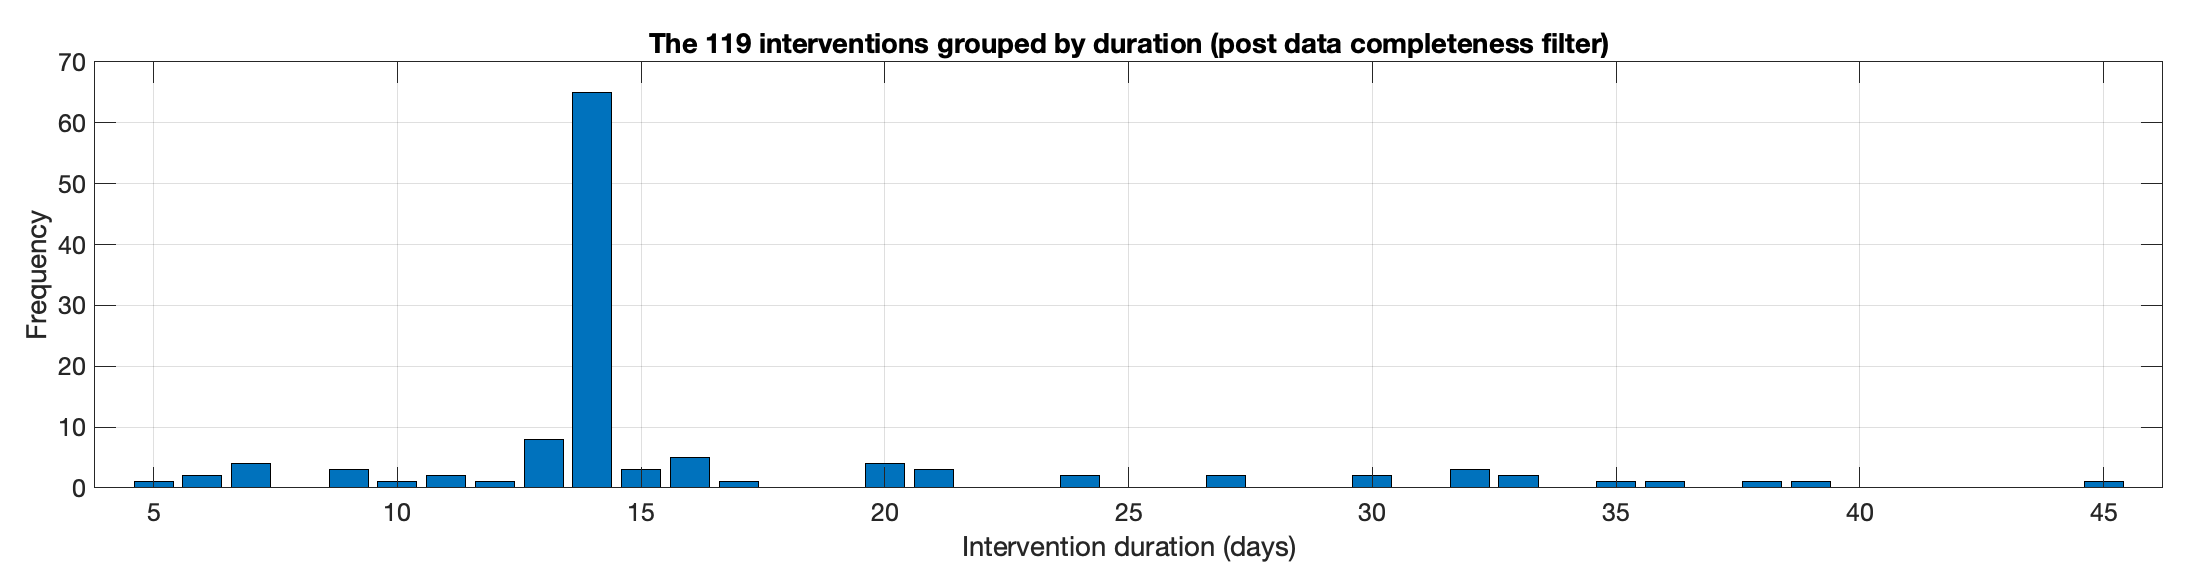
\includegraphics[width=150mm]{images/intrduration.png}
    \label{fig:intrbyduration}
    \end{figure}

    \item It should be small enough to have a sufficient amount interventions. Due to the scarcity of the data, the choice of D and the criteria for "insufficient data" stated in \ref{sec:intrlist} closely work together to define the amount of selected interventions, as shown in the table below.
    
    \vspace*{5px}
    \begin{center}
    \begin{tabular}{c|c} 
    \hline
        \textbf{D} & \textbf{Filtered interventions} \\
        \hline
        20 & 119 \\
        40 & 55 \\
    \hline
    \end{tabular} 
    \end{center}
    \vspace*{5px}
    
   This confirmed the choice for D = 20. 119 interventions is already a small sample size. In particular, the aim is to split the data in two or more folds, while learning different latent curves, a high amount of interventions is critical.

\end{itemize}

\subsection{Model dimensionality}
The number of bio-markers chosen is exactly the number of dimensions that will be studied by the model. The measures mask (mm) parameter filters a subset of M measures out the 18 listed in table \ref{tab:measures}. Note that \textit{measures} and \textit{bio-markers} from the biological vocabulary, and \textit{features} from the machine learning vocabulary are used as synonyms.

The rule of thumb to chose the model dimensionality is dual:
\begin{enumerate}
    \item Patients are a complex system whose behaviour is expected to be inferred using different types of features. This complexity can be met by increasing the data dimensionality. Unless bio-markers are extremely noisy and not correlated with the patient's status, they are kept. From thorough observation, calories, weight were removed because noisy and uncorrelated with events. Pusle rate was found to be more correlated to the recovery than resting heart rate. Minutes asleep and temperature seemed not correlated but were kept in doubt.
    \item Measures of the same family, e.g. "forced expiratory" based measures (FEV1, FEV6, FEF2575, etc) or subjective measures (wellness, cough), contain a similar patient information. Since each measure has the same weight in the calculation of the objective function, the model can be biased if one family is over-represented. To avoid point 2., only two measures from the FEV family were kept: FEV1 as a) it was the signal with clearest behaviour and b) it is the gold standard for respiratory measures in cystic fibrosis studies \cite{giron_2021}. FEF2575 was also used since a) during optimisation it showed increase model numerical stability and provided a lower objective function at end-state (average of 1.3 without and 1.27 with based on 13 runs), b) clinically it can provide more consistent signal than FEV1 for asymptomatic patients, whose number is subject to rise after the transition to the highly effective Trikafta CFTR modulator.
\end{enumerate}

Therefore cough, wellness, FEV1, FEF2575, pulse rate, O2 saturation, temperature, minutes asleep were selected, i.e. 8 dimensions.

A data density check was performed to avoid numerical instability on the typical profile. This could happen if there was a generalised absence of measurements at specific times from treatment accross all patients. Fore example during hospital intravenous antibiotics (IVs), the patient might be constrained by fatigue or equipment for some measurements (weight, spirometry). The heatmap of the measurements for all intervention on figure \ref{fig:heatmap} present an homogeneous at an intervention level and no specific patterns in the columns that could be expected.

\begin{figure}[!h]
    \caption{Heatmap of the amount of measurements recording (mm=34) for each intervention (line) and day in range [-25;39] around treatment start (1 pixel is one day)}
    \centering
    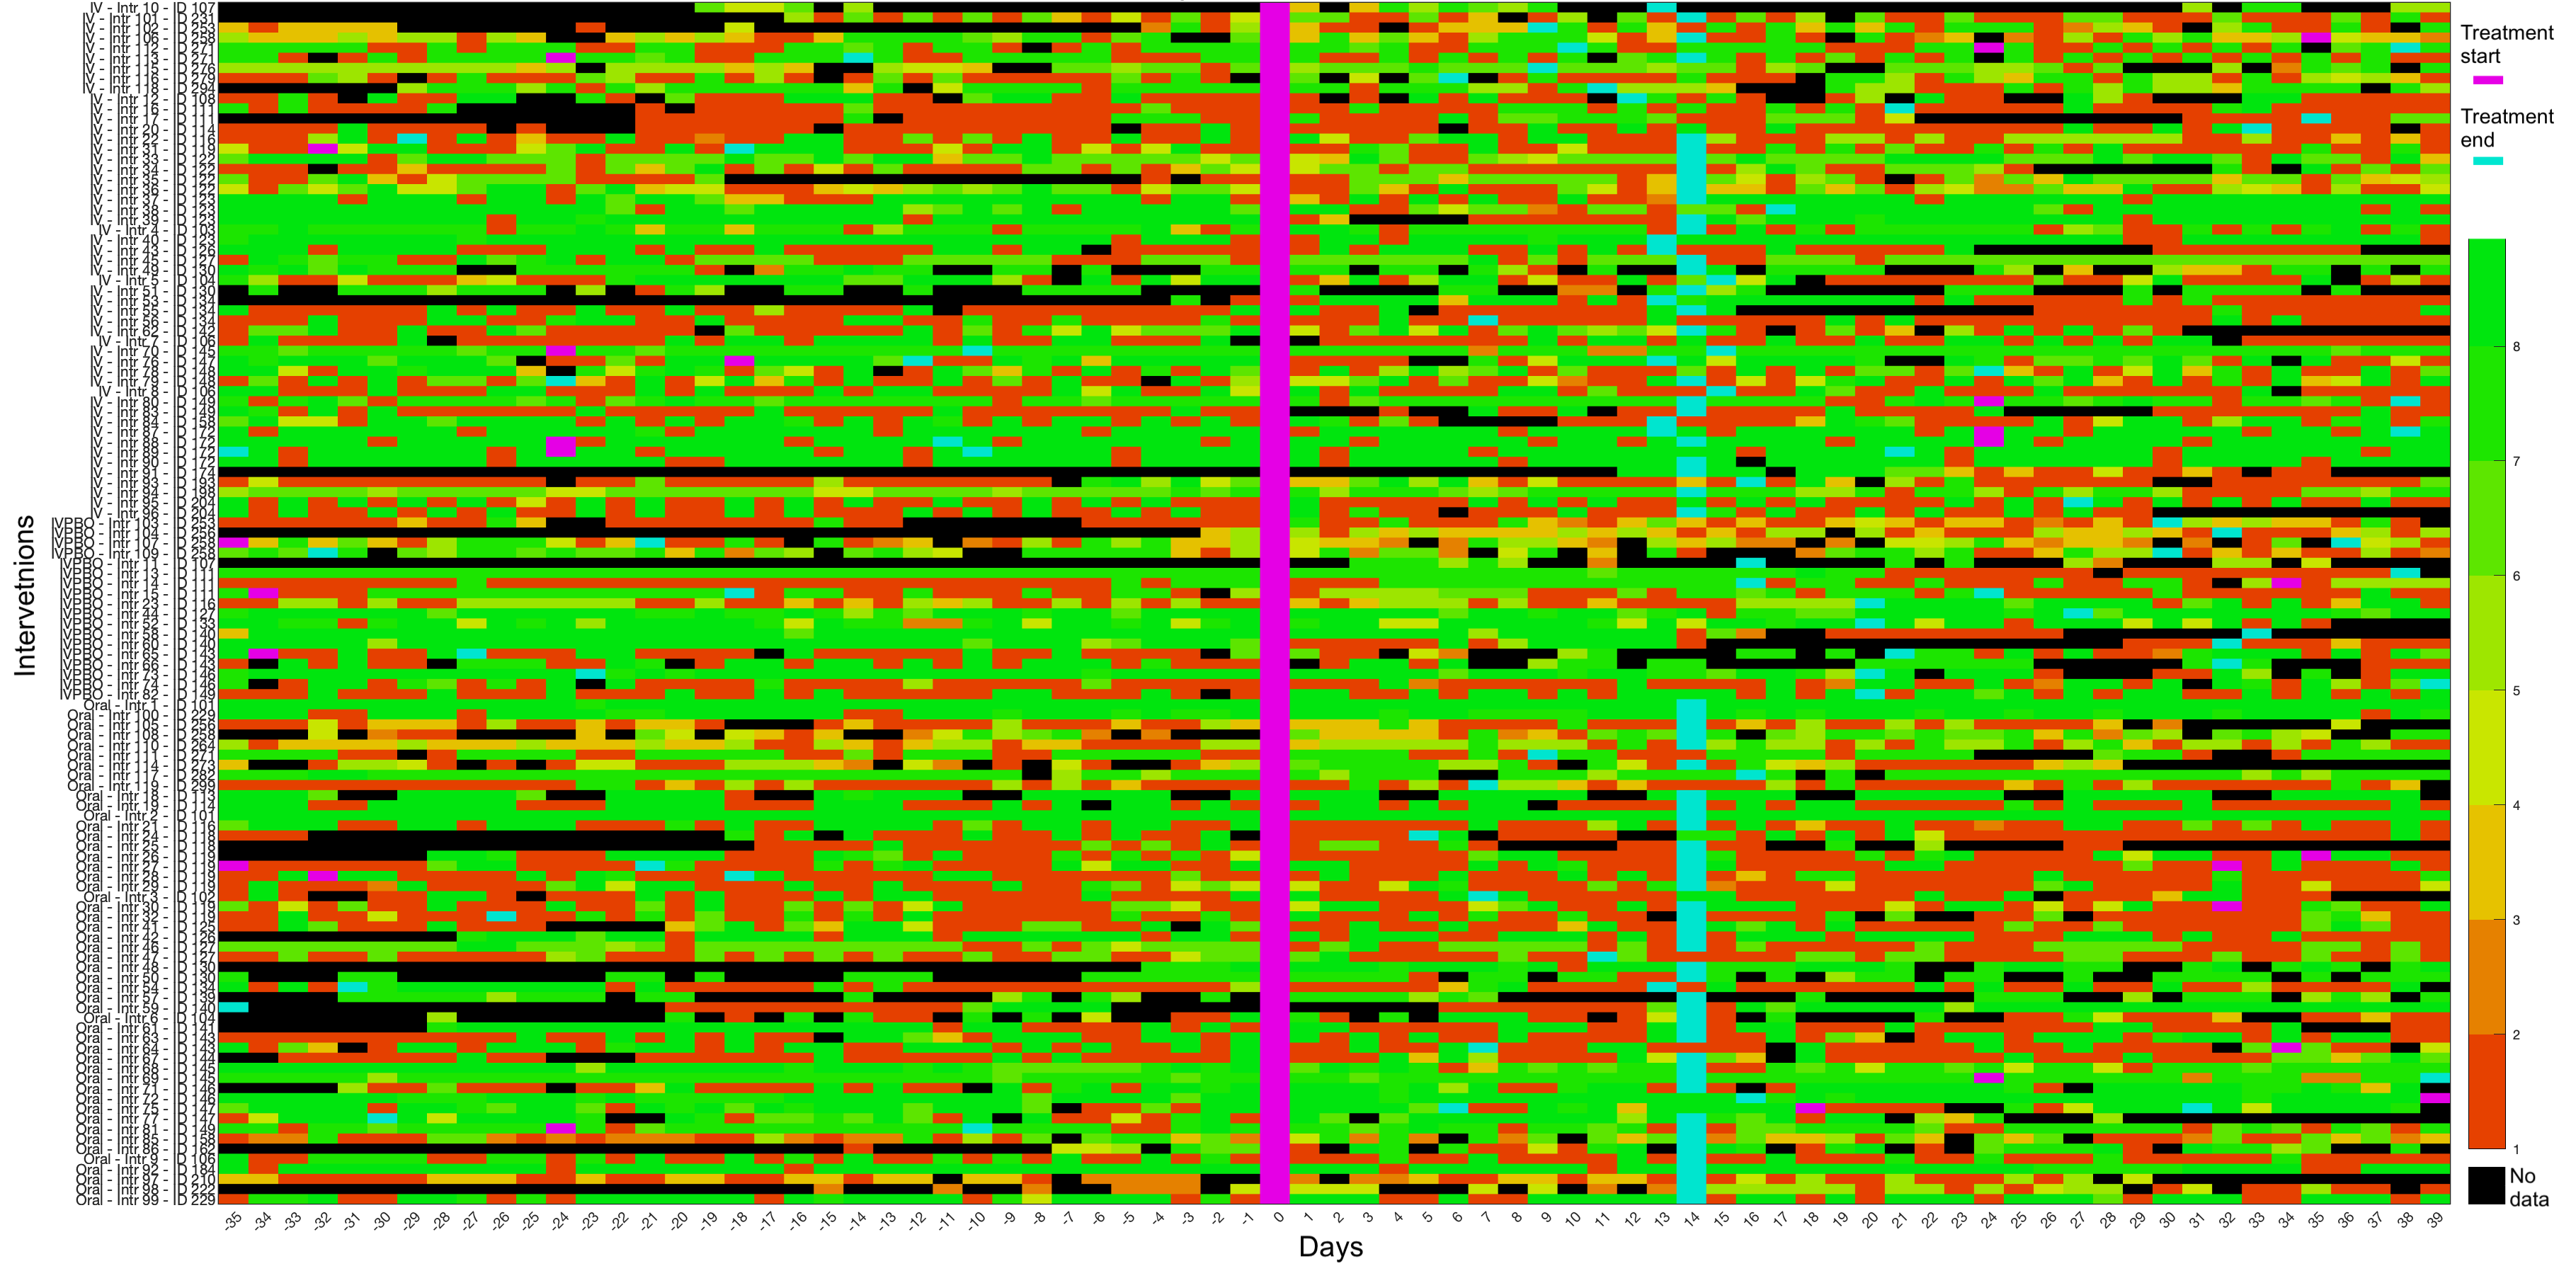
\includegraphics[width=150mm]{images/heatmapmm.png}
    \label{fig:heatmap}
\end{figure}

\subsection{Maximum offset}
The choice of this parameter is a trade-off between 1) minimising the objective function, 2) while having a sufficient point contribution for each day on the typical profile (chosen as at least 5 for one curve - referred to as \textit{count threshold}). For 1), the greater the offset the smaller the final objective function's value, see figure \ref{fig:offsets}. Issue 2) will arise on the left-most part, poor in data records contribution due to the right-shift without left-wise data imputation. The maximum offset was chosen by sequentially increasing its value and looking at the resulting typical profile, until the typical profile was imprecise on the left. mo > 16 lead to empty slots on the left-most part of the typical profile for FEV1 and wellness, see grey bar graph on figure \ref{fig:offsets}. FEV1 and wellness were chosen because they were representative of the other measures and subject to missing data (the median for the density of measurement over the whole study were respectively 19\% and 22\%, meaning 1.4 measurement per week). Therefore mo is set to 15.

\begin{figure}[!h]
    \caption{Maximum offset benchmark with inferred FEV1, wellness typical profiles for $mo \in \{10, 15, 16\}$ }
    \centering
    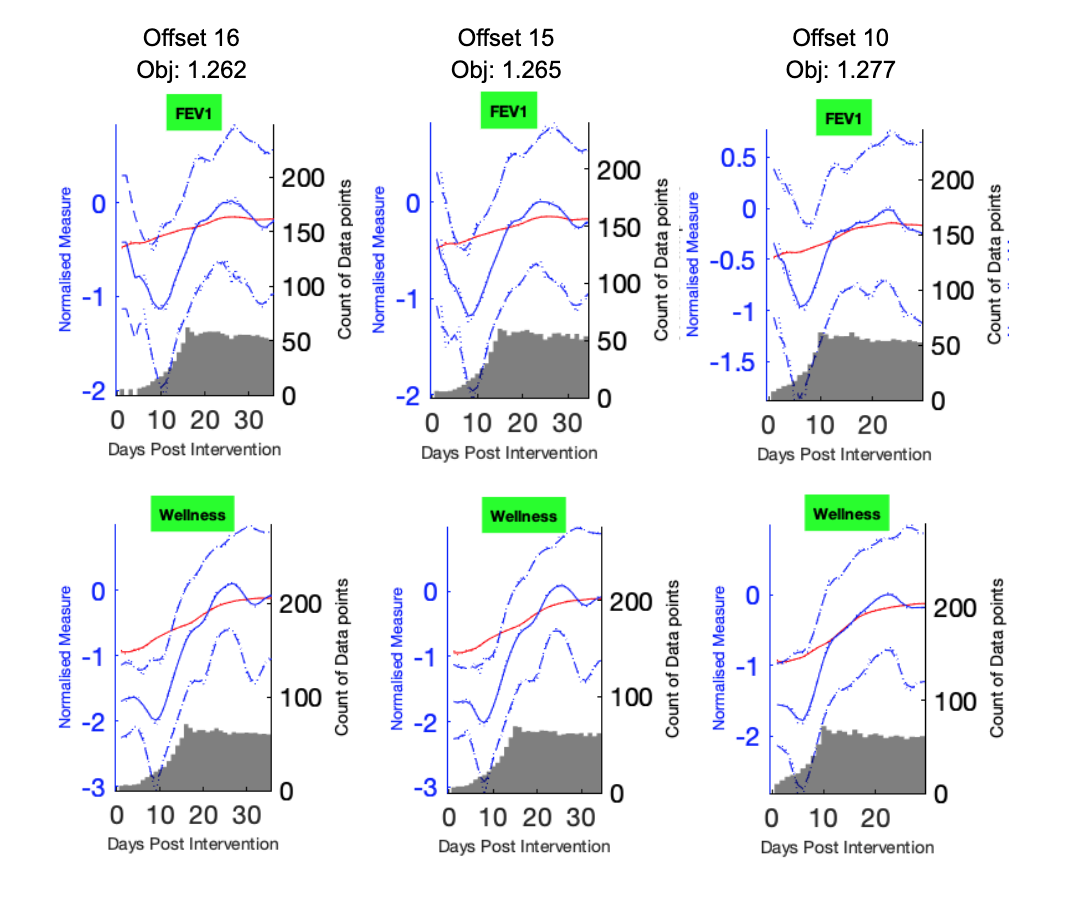
\includegraphics[width=90mm]{images/offsets1.png}
    \label{fig:offsets}
\end{figure} 
Note: on figure \ref{fig:offsets}, the blue curve is the typical profile (with mean in plain line and standard deviation in dotted line), the red curve indicates the unaligned profile, i.e. with all offsets forced to 0, and each grey bar in the bottom chart is the amount of data points contributing to the corresponding day on the typical profile.

\subsection{Maximum vertical shift}
The maximum vertical shift ($\alpha$ as defined and described in \ref{sec:vshift}) is fixed by running several models and comparing 1) the trend of the typical curve, 2) the distribution of vertical shift allocation. On the distributions, for the data records where the vertical shift is between the boundaries, the remaining vertical shift between the sample and the typical profile is fully cancelled. At the boundaries, the difference in mean is adjusted by $\alpha$ thus strengthening the importance of the underlying evolution in recovery over the difference in mean.
One can observe on figure \ref{fig:vshift} that the sensibility of  wellness (and also cough, minutes asleep, O2saturation, temperature) is low with respect to vertical shift. However, there is a minimum vertical shift of 0.4 necessary to allow to differentiate data records based on FEV1 (also generally all FEV measures and pulse rate). As two high values for this parameter cancel the difference of mean that can help differentiate two recoveries (\ref{sec:vshift}) $\alpha$ was set to 0.4 for the rest of the study. This is also the standard value used for the APE study \cite{damian}. Note that for two classes inference  $\alpha = 0.4$ is the value corresponding to the most robust model, see section \ref{sec:robustness}.

\begin{figure}[!h]
    \caption{Vertical shift benchmark with distribution and inferred FEV1, wellness typical profiles for $\alpha \in \{0, 0.2, 0.4, 0.7\}$ }
    \centering
    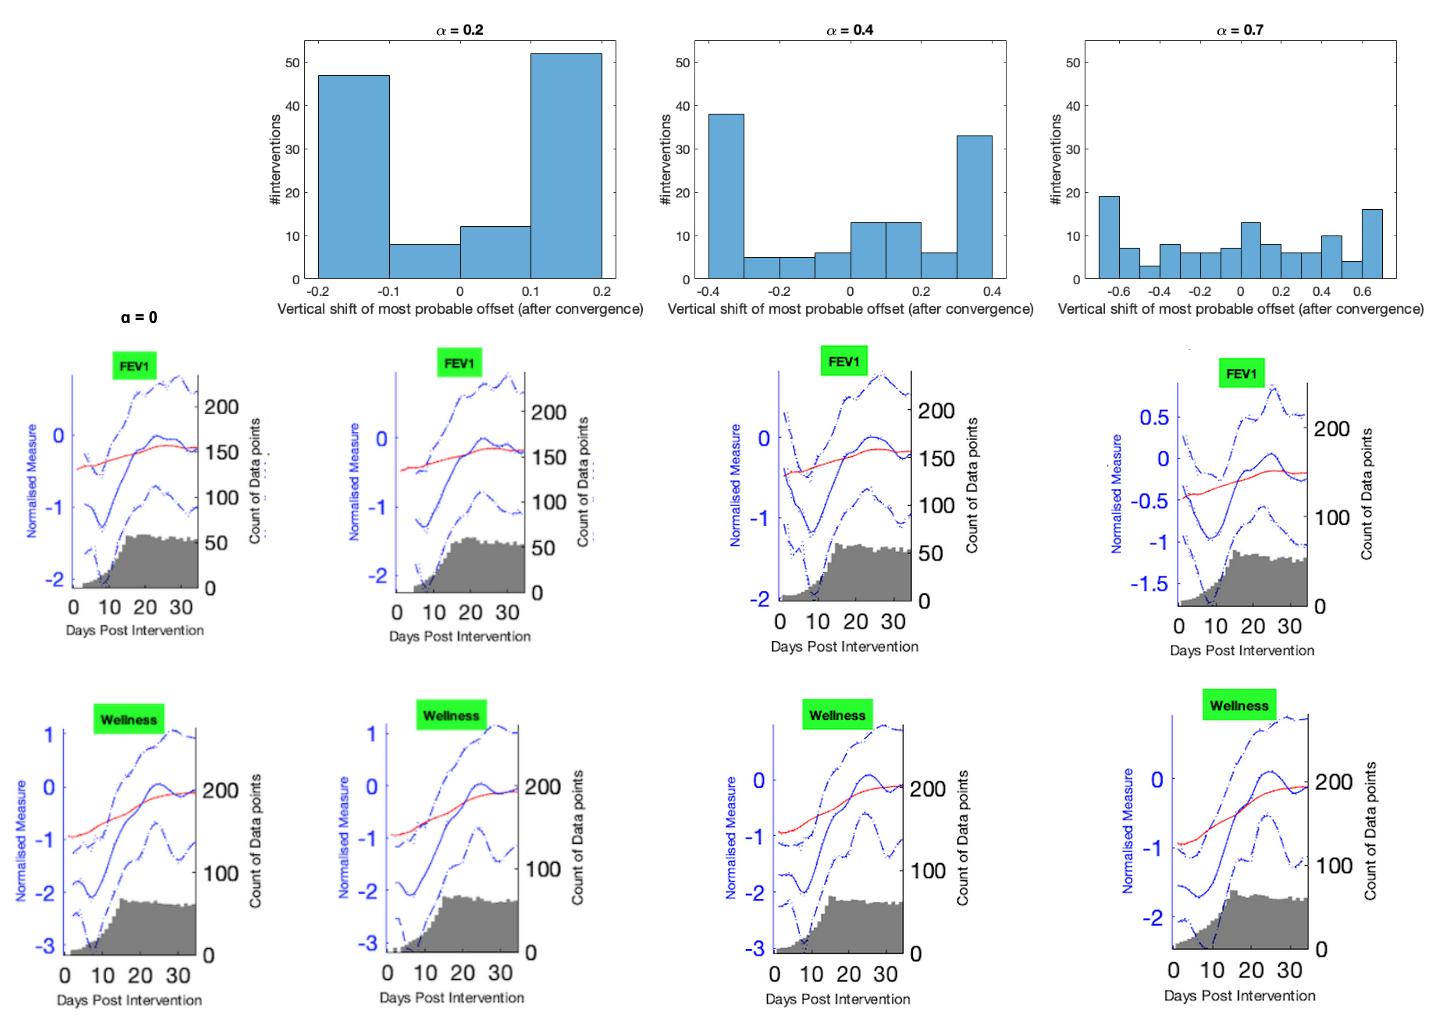
\includegraphics[width=140mm]{images/vshift.png}
    \label{fig:vshift}
\end{figure} 

\section{Generation of the typical recovery profile}
Given the chosen core parameters in \ref{sec:chosenparam}, the typical profile is drawn on figure \ref{fig:profile}. It is important to remember that the profile does not contain data prior to treatment start. 
\subsubsection{Graphical settings}
No vertical adjustment of the profiles were done. Therefore, the 0 on the y-axis corresponds to the stable baseline as defined in \ref{sec:normalisation}. The curves were smoothed with a 3 days window to filter day to day noise and improve the clarity of the final graph. Some left-most points are missing: there were not plotted because less than five data records' values contribute to them, i.e. there is too much uncertainty about their typical value. The typical curve for FEF2575 and temperature were not plotted because the first it had a very close behaviour to FEV1, and the latter did not seem to contain information related to the recovery.

\begin{figure}[!h]
    \caption{Typical profile derived with the probabilistic inference algorithm, with 119 data records}
    \centering
    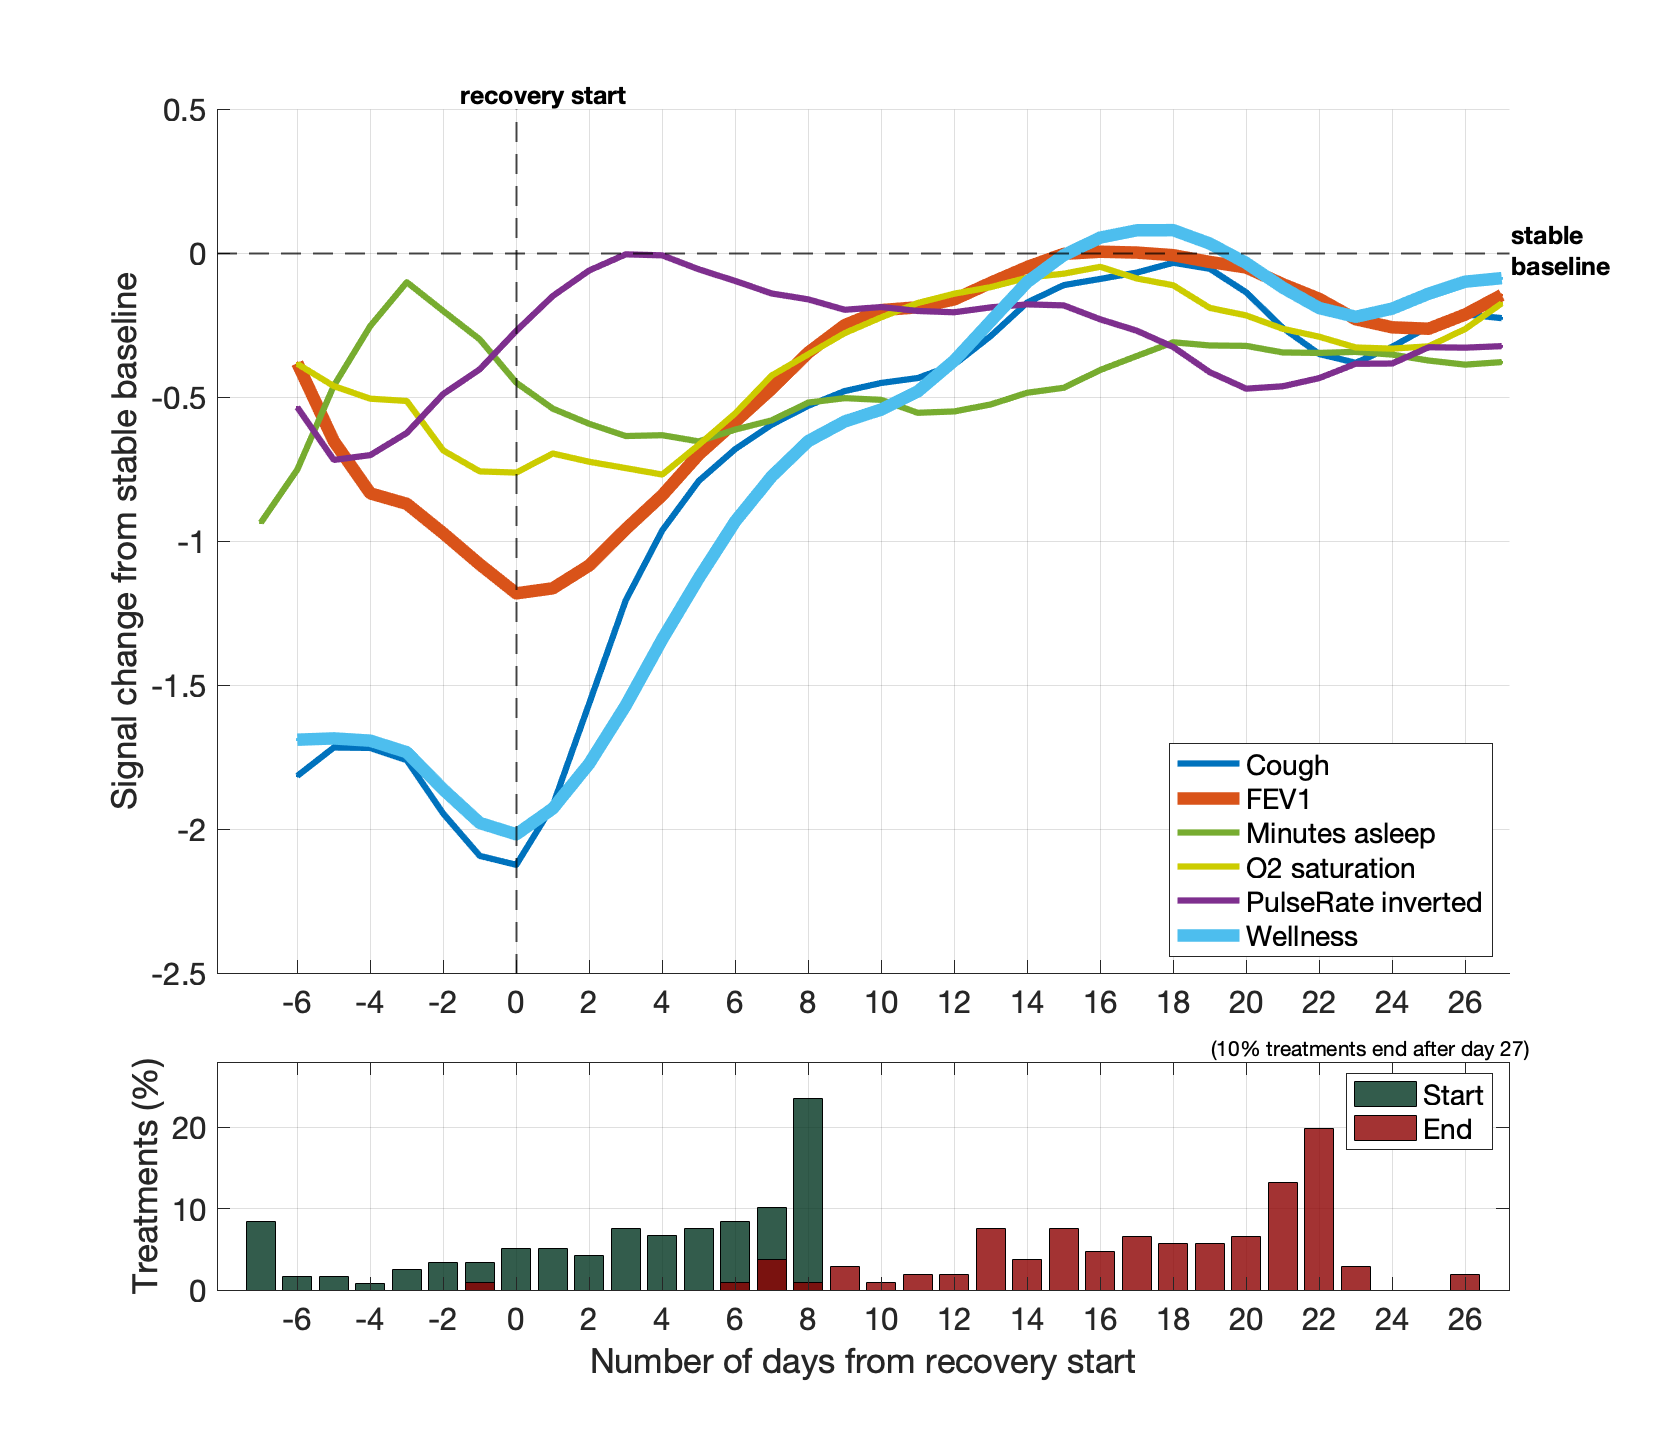
\includegraphics[width=100mm]{images/profile_typical.png}
    \label{fig:profile}
\end{figure}

\subsection{Terminology}
The terms used to analyse the recovery profiles are introduced here.

\textbf{Recovery start ($k_R$)} is defined to be the consensus beginning of increase for all measures. If unclear, a higher weight is given to FEV1 and wellness (highlighted with a thicker line on the graphs), which show the clearest contrast. At measures level, the recovery start is the beginning of increase for that measure. Any treatment starting after $k_R$ has a recovery start on the same day as the treatment start. Note that one can expect continuous decline that can sometimes be clinically explained by antibiotic resistance of the infection participating bacteria. In such cases, the recovery start is undefined.

\textbf{Time to (treatment) response ($\tau$)}: It is equal to the number of days between treatment start and recovery start. Based on our model, it can be computed for each intervention n with the offset $F_n$ and the recovery start $k_R$:
\begin{equation}
    \forall n \in N, \tau = 
    \begin{cases}
        k_R - F_n & \text{for } F_n < k_R\\
        0 & \text{for } F_n \geq k_R\\
    \end{cases}
\end{equation}
A time to treatment response of 0 means that the treatment had an effect on the signals within the day it was started.

%The values of the signals are in a
%\textbf{Recovery from partial decline:}  At treatment start, the signals are 

\textbf{Full recovery:} After treatment start, the signals come back to the stable baseline.

\textbf{Partial recovery:} After treatment start, the signals increase but do not come back to the stable baseline, i.e. the recovery is not full. This is an example of unsuccessful recovery.

\textbf{Successful recovery:} A recovery is defined as successful when the measures come back and stay "close" to the stable baseline. In literature, "close" is defined as 90\% of the stable baseline \cite{morgan_2017}.

The limit between \textbf{full decline} and \textbf{partial decline} is defined for reach signal at 25\% of the height between the lowest signal's point and the stable baseline. Looking at the typical profile, if most measures' profile contain values below the limit, the recovery starts from a full decline. Else, the recovery starts from a partial decline.

\subsection{Typical recovery profile observations}
The main concept behind the typical profile for recovery is that any D-day long physiological time-series immediately following a treatment can be placed on the matching measure of this profile with little error. Interventions that do not fit are considered as atypical with respect to this profile. This is reformulation of the model's first assumption defined in \ref{sec:datagen}. Looking at figure \ref{fig:profile}, one can note the following points:
\begin{itemize}
    \item FEV1, cough, wellness, O2 saturation have a closely similar behaviour with different amplitude.
    \item ~40\% of the recoveries start from a full decline, ~60\% from a partial decline, based on FEV1, cough and wellness.
    \item All patients' typically recover fully 14 days after the recovery start. There is a clear recovery climax 15-20 days after treatment start. After this, the signals undergo a call-back (slight decline) prior to their stabilisation.
    \item There is no sign of sharp decline after treatment end.
\end{itemize}

\subsection{Typical time to response}
The response to treatment $\tau$ is computed for all interventions on figure \ref{fig:tau}, based on the computed offsets and the determined recovery start. For over 90\% of the interventions, the response to treatment is 0, i.e. the recovery starts on the same day as treatment start. Note that the time to response can also be read on the bar graph of the treatment start, it is the gap in days between the treatment start and the recovery start.

\begin{figure}[!h]
    \caption{Typical time to response}
    \centering
    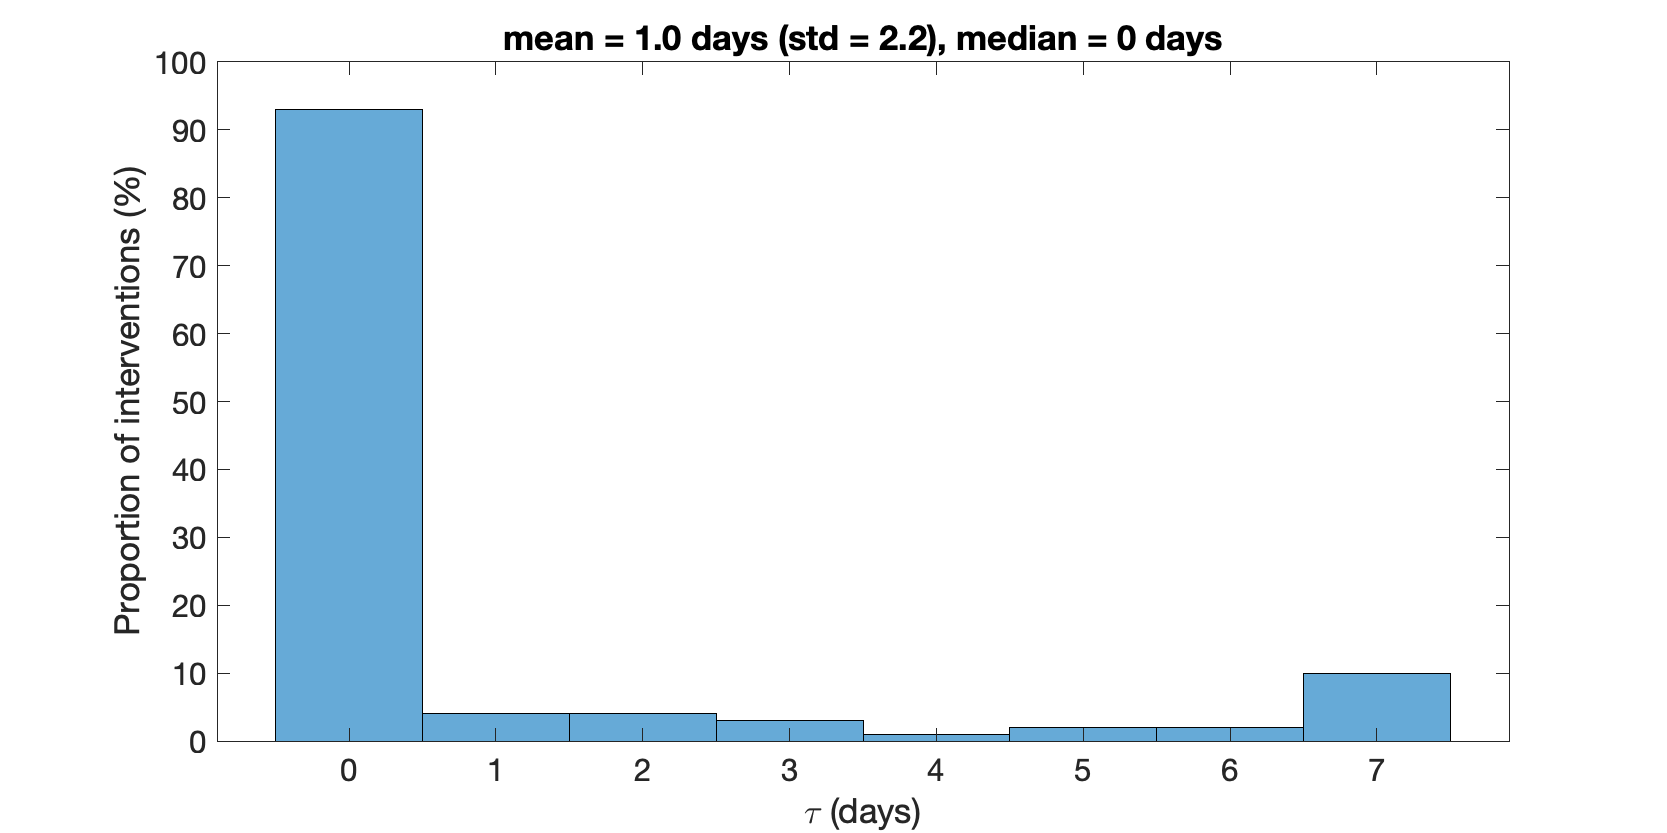
\includegraphics[width=90mm]{images/tautypical.png}
    \label{fig:tau}
\end{figure}

\section{Different types of recovery inference}
Now that the foundation of the typical profile was built, one would like to answer the question "Are there different types of recoveries?". The main interest is to create knowledge for the clinician. In this section, two types of recoveries are inferred and then mapped to patients' specificity, e.g. microbiology and lung volume. Additionally, the typical profile of an unsuccessful recovery is drawn.

\subsection{Model robustness}
The robustness against initialisation is the capacity of the model to provide the same end-states amid various initialisation-states. In the current settings, as all data records are randomly initialised to a class, and the end state is the mapping $\mathcal{F}$ described in \ref{sec:multiclass}. The robustness of the model was evaluated by initialising the model with different random seeds and comparing the end-states, for two latent curves.

\subsubsection{Class labels harmonisation with 2 latent curves}
Since the initialisation is random, the end-states are class-agnostic. In fact, the interventions corresponding to first class for one random seed can match the interventions corresponding to the second class of another random seed. Among the used random seeds, the set of interventions that had most in common with the class 1 of an end-state taken as reference were set to class 1 and the others were set to class 2.

\subsubsection{Model robustness for 2 latent curves} \label{sec:robustness}
The model was run 14 times with 7 different random seeds and 2 different maximum vertical shift, and a maximum iteration number of 120. When the maximum number of iterations was reached, results were taken as valid only if offset and latent curves had not changed since more than 5 iterations. Results for $\nu=0.4$ are given in table \ref{tab:nl2vs}. The random seed that minimised the objective function was taken as reference, e.g. rs1 for $\nu=0.4$. Figure \ref{fig:nl2classerror} shows the classification error for the corresponding end-state. An intervention with n errors was assigned \textit{n} times to the wrong class, and \textit{7-n} times to the right class. N=3 concerns outlying interventions, consistently switching between classes.

Relatively, $\nu=0.4$ is more optimal than $\nu=0.7$. Whereas $\nu=0.4$ provided 6 outlying interventions and over 80 interventions with 1-error or less, $\nu=0.7$ provided 19 outlying interventions and more 2-errors than 1-errors.

Globally with $\nu=0.4$, the model was considered as robust enough. In fact, for random seeds 1, 3, 5, 6, 7, a baseline of 72\% of interventions, were systematically belonging to the same class. The 5\% outlying interventions were also systematically the same, namely \{8; 41; 55; 94; 102; 104\}. Those outlying interventions did not show related characteristics, based on patient number, route, average measures per day, days with measures, offsets, and drug therapy. The resulting 23\% of interventions were switching between class 1 and class 2 depending on the initialisation state, highlighting slightly different relation between the features.

Hence, the model was consistent enough to infer two types of recoveries with $\nu=0.4$ and random seed 1, which provided the minimum the objective function.

\begin{figure}[!h]
    \caption{Classification error for $\nu$ = \{0.4; 0.7\}}
    \centering
    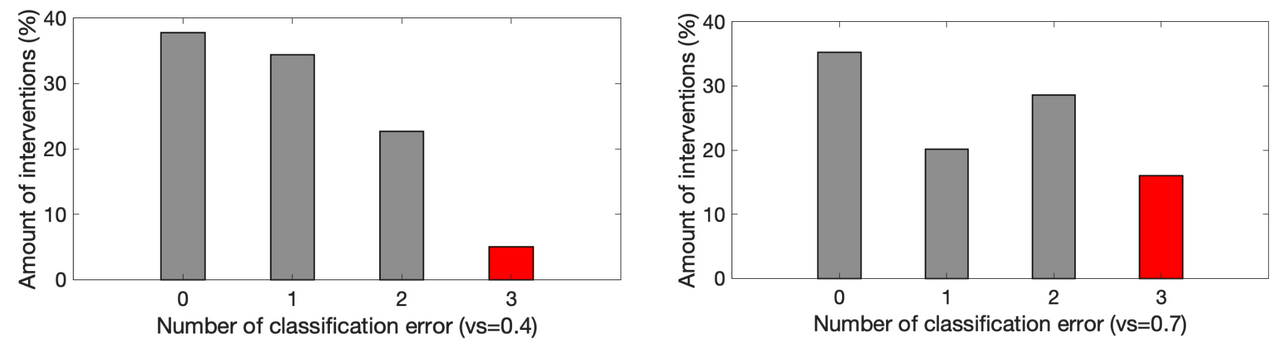
\includegraphics[width=100mm]{images/nl2classerror.png}
    \label{fig:nl2classerror}
\end{figure}

\begin{table}[!h]
    \centering
    \begin{tabular}{c|c|c|c|c|c|c}
        \hline
         \textbf{Random seed}& \textbf{Obj} & \textbf{Class 1} & \textbf{Class 2} & \textbf{ $\leq$ 1 error} & \textbf{3 errors} & \textbf{Iterations}\\
         \hline
         rs1 & 1.2243 & 63 & 56 & 72\% & 5\% & 120 \\
         rs2 & 1.2316 & 57 & 62 & 70\% & 5\% & 58 \\
         rs3 & 1.2313 & 43 & 76 & 72\% & 5\% & 120 \\
         rs4 & 1.2297 & 55 & 64 & 59\% & 21\% & 120 \\
         rs5 & 1.2283 & 42 & 77 & 72\% & 5\% & 91 \\
         rs6 & 1.2255 & 39 & 80 & 72\% & 5\% & 120 \\
         rs7 & 1.2306 & 39 & 80 & 72\% & 5\% & 120 \\
         \hline
    \end{tabular}
    \caption{Model run results for 7 different initialisation-states, $\nu=0.4$}
    \label{tab:nl2vs}
\end{table}

%Through each iteration, the algorithm then allocates the samples (data records) to the current best matching unit (latent curve). After convergence, the end-state is the mapping $\mathcal{F}$ described in \ref{sec:model}. 

%The inferred classes with n latent curves are a n-fold partition of the 119 data records. 

\subsection{Two distinct typical recoveries}
The model was run to infer two distinct classes of recoveries. Given the model's robustness analysis, the core parameters and graphical settings were chosen identically to the ones for the typical profile.

The class 1, figure \ref{fig:profileC1C2}, show interventions with partial recoveries. ~77\% of recoveries start from a full decline (days [-11; 2]). The time to response is highly left-skewed with a maximum of 11 days. There is a similar call back to the one on the typical profile.

The class 2, figure \ref{fig:profileC1C2}, show very different behaviour. Wellness, cough and FEV1 show a full recovery at day 9, therefore much earlier than on the typical profile, that goes beyond the stable baseline and far higher than on the typical profile. One can note that pulse rate does not show to be related to the recovery. ~43\% of recoveries start from a full decline (days [-6; 2]). The time to response is left-skewed with a maximum of 6 days.

\begin{figure}[!h]
    \caption{Class 1 profile with 53\% of data records (left), Class 2 profile with 47\% of data records (right)}
    \centering
    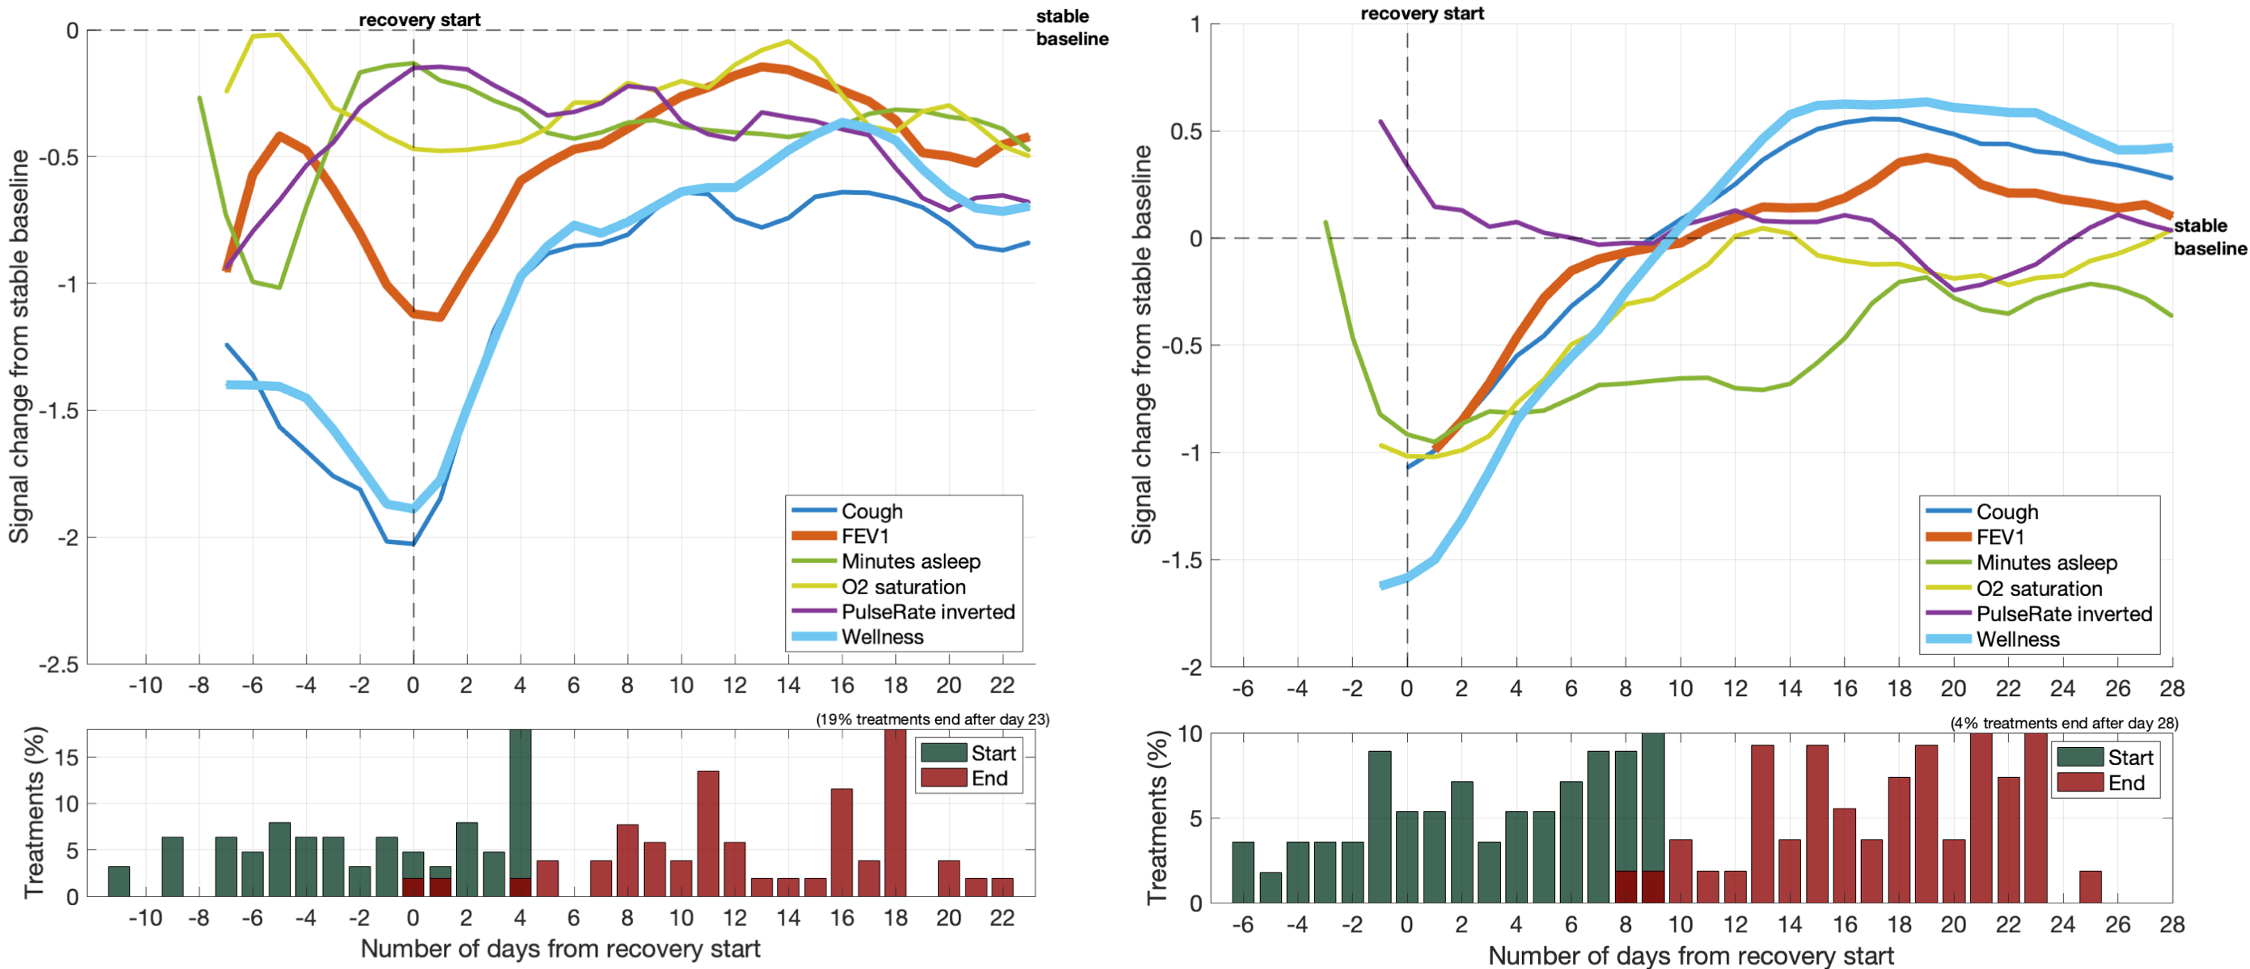
\includegraphics[width=160mm]{images/nl2.png}
    \label{fig:profileC1C2}
\end{figure}

\subsection{Relation with patients characteristics}
Relation between patients' characteristics and classes were computed through hypothesis testing, after removing the 6 outlying interventions. Wilcoxon signed-rank test was used to test the null hypothesis that data in Class 1 and Class 2 are samples from continuous distributions with equal medians. Chi-Square Goodness-of-Fit test was used to test the null hypothesis that the data in Class 1 fits the distribution of the data in Class 2. This was used for binary data, e.g. sex, presence of an infection, as the distributions need not be continuous. A significance level of 0.01 was chosen to limit the amount of type II errors. 

In the results of the hypothesis tests summarised in figure \ref{fig:pvalue}, Class 2 recoveries are more commonly found in people with a high number of antibiotic treatments and in particular IV treatments over the study period. Note that class 1 and class 2 contained IV or Oral treatment in balanced proportion, roughly half-half. People with chronic pseudomonas aeruginosa infections more likely to experience recoveries of Class 2. 

    \begin{figure}[!h]
    \caption{Hypothesis tests results, for $\alpha=0.01$}
    \centering
    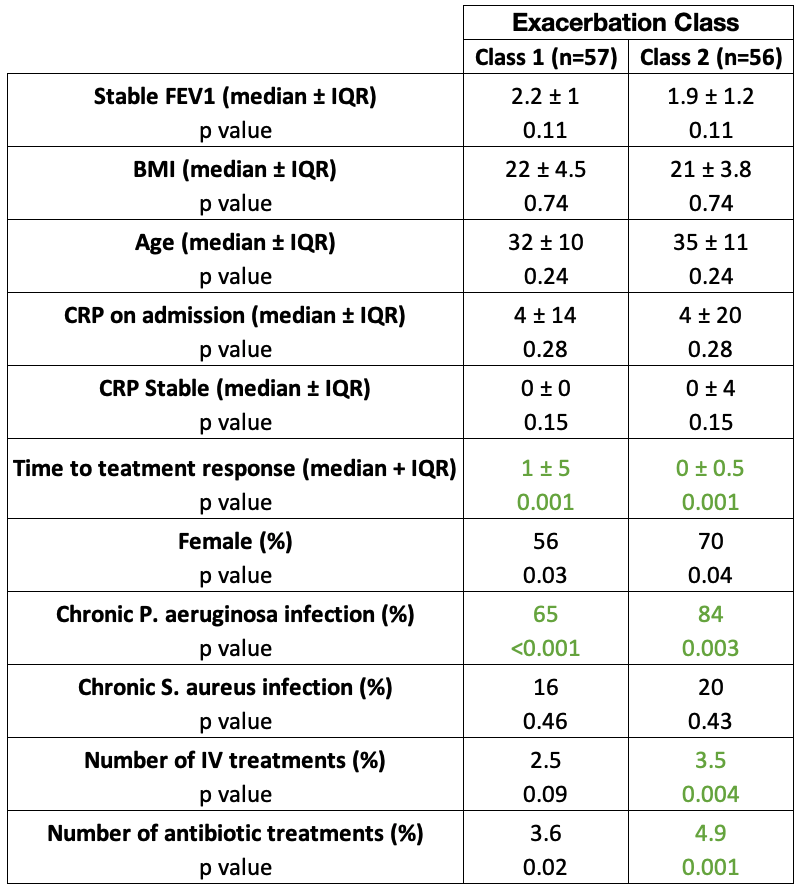
\includegraphics[width=70mm]{images/pvalue.png}
    \label{fig:pvalue}
    \end{figure}

\subsection{Typical profile of a full recovery with decline}
The previous analyses did not present clear signs of a special type of unsuccessful recovery where the signals undergo a full or almost-full recovery swiftly followed by a clear decline. Clinically, this is commonly known in the case of repeated APEs, where the patient degrades again right after treatment. One could wondered whether the model can also be used to characterise this type of recovery.

While observing the data records, 35 cases showed a decline before or after the end of the treatment. A model was run with this subset of interventions. On figure \ref{fig:fail}, most signals including FEV1 undergo a slight increase from day -2 to day 12 up to the stable baseline, followed by a decrease of same amplitude from day 12 to day 32. Note that the consensus decline start on day 20 happens when ~40\% of treatments are not finished. Cough and wellness are the only measures with a clear increase as a response to treatment. Also, ~25\% of treatments start after day 8 of this profile, and are characterised by an absence of response to treatment. 

\begin{figure}[!h]
    \caption{Typical profile of a recovery with decline (30\% of interventions)}
    \centering
    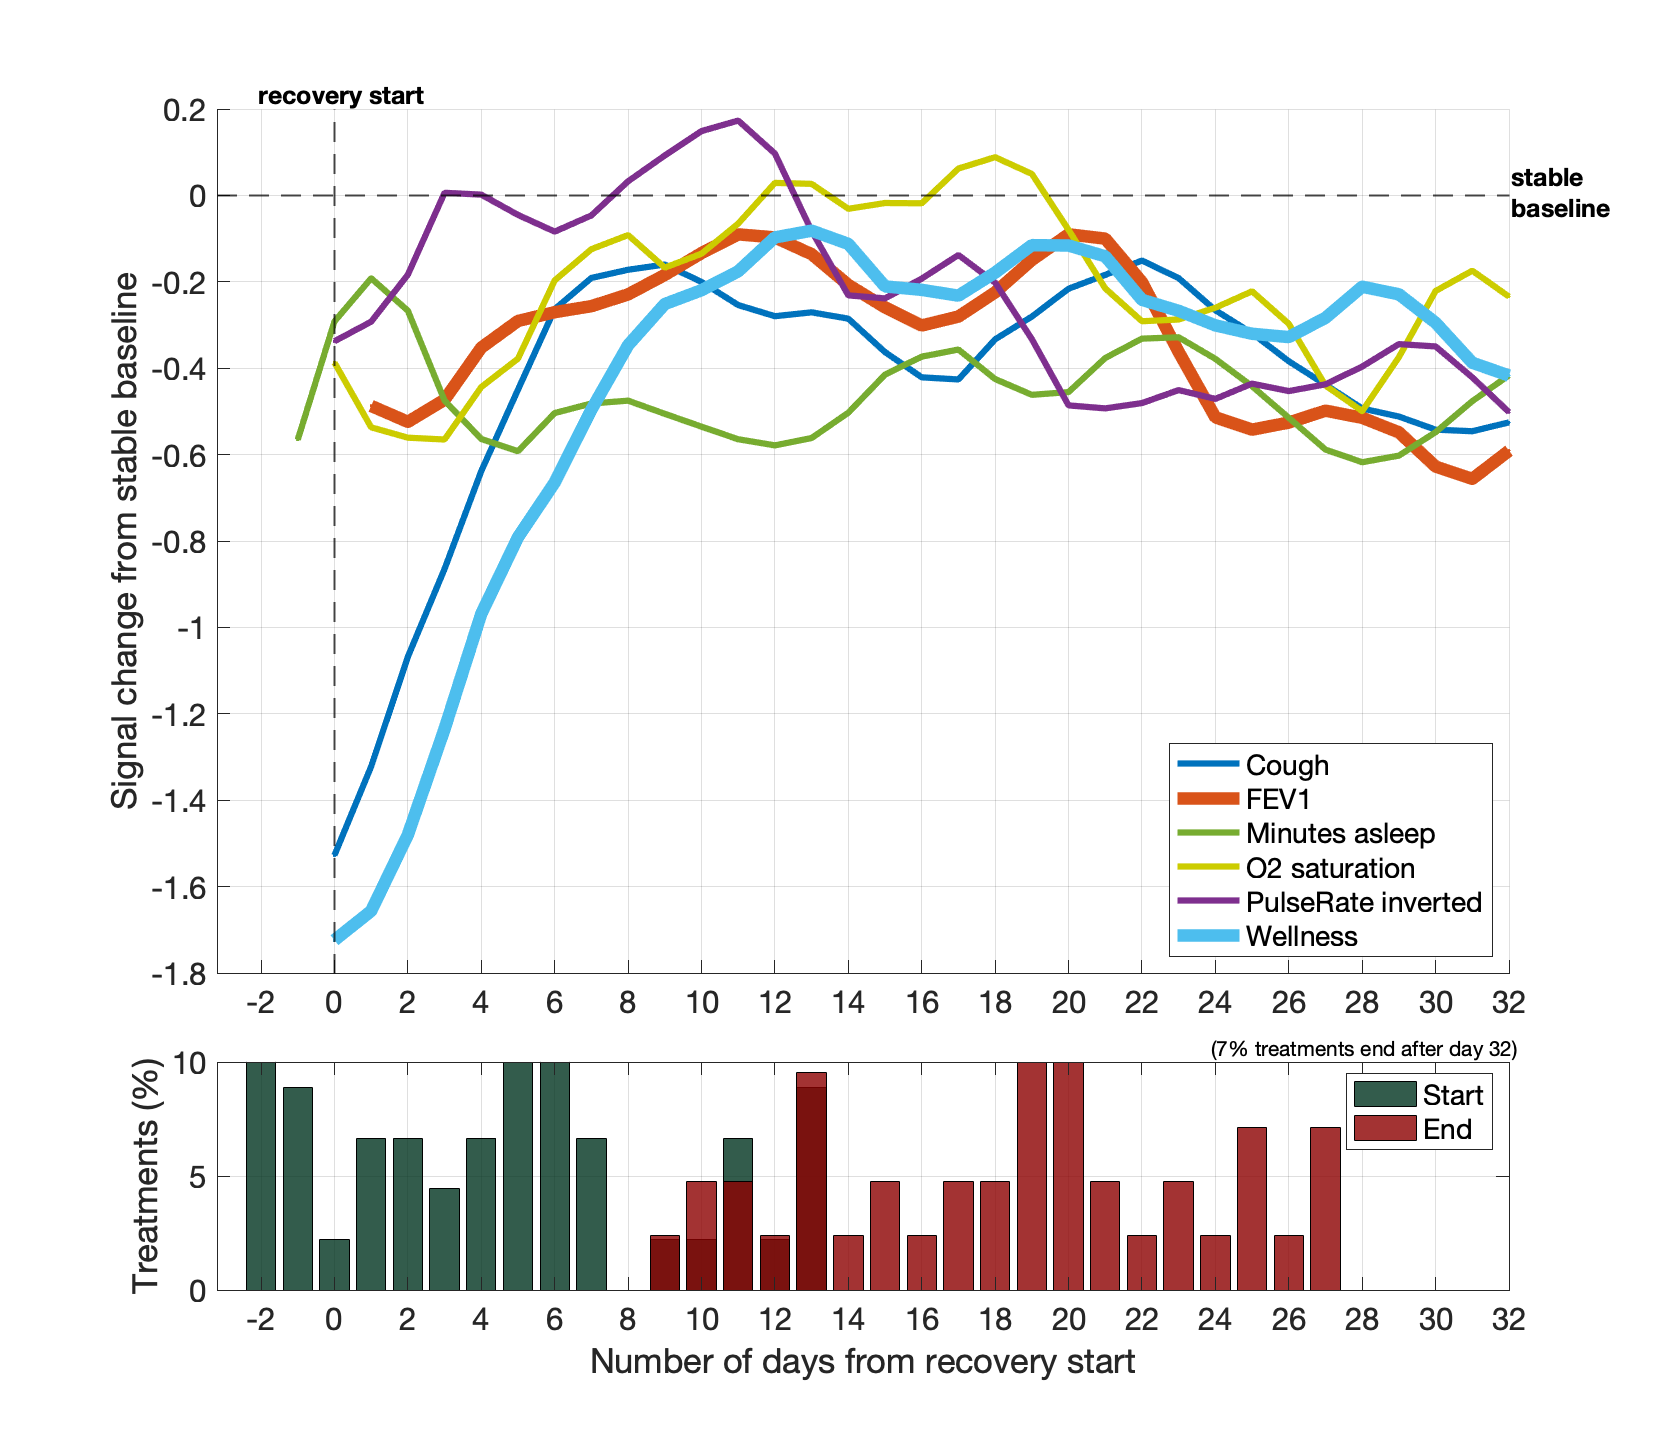
\includegraphics[width=100mm]{images/profile_fail.png}
    \label{fig:fail}
\end{figure}

\section{Recovery definition}
Thanks to the previous results and observation, a recovery can be defined as as follows: 

\definition A recovery is a process of change in the patient's health status following an antibiotic treatment, closely linked to the preceding acute pulmonary exacerbation. It lasts from the treatment start until the day where a recovery label can be assigned with sufficient certitude. A recovery can be analysed through the observation of different sets of physiological bio-markers. Elective treatments are defined as treatments that seemed not preceded by an APE.

The recovery label can be set according to the process on figure \ref{fig:types}. Example for a label: "unsuccessful partial recovery from full decline".

\begin{figure}[!h]
    \caption{Directed graph that can be used to label recoveries}
    \centering
    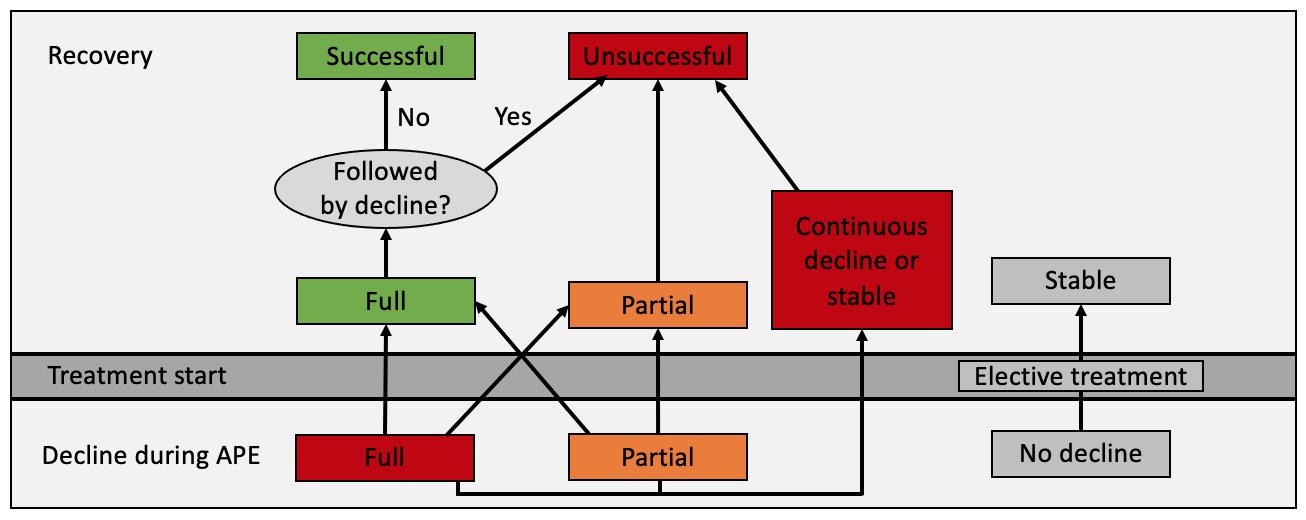
\includegraphics[width=130mm]{images/types.png}
    \label{fig:types}
\end{figure}



%\section{Slope based classification of a recovery}
%Based on our analysis, 
%When we asked ourselves the question "What is a recovery from antibiotics?", it appeared that there was no clear classification nor definition of the different types of recoveries. Clinicians can easily list the different types of recoveries from antibiotic treatments based on their multi patient experience, but we are unsure if there nuances or consensus in the clinician community. We suggest that during each clinics following an antibiotic treatment, recoveries could be labelled according to this classification. Similar longitudinal evolution of the recovery labels could help group patients together and treat them according

%From a clinical perspective, we can expect different types of intervention summarized in the following table:
%Literature well defines everything linked to a recovery, but not the recoveries themselves. Classifiation of 
\chapter{Discussion}

\section{Results interpretation}
The recovery-specific questions "How does a recovery look like?, "Are there different types of recoveries?" were answered with the probabilistic inference algorithm. The characterisation of recovery's summary that can be provided to CF specialists is described in this section.

\subsubsection{Typical recovery profile}
A characteristic profile of the changes in physiology and symptoms during a recovery was generated using a Bayesian inference algorithm with expectation maximisation. The profile allows to define an accurate recovery start date, which provides a label to explore the time to response, and the quality of the recovery.

The typical recovery profile revealed that health bio-markers typically respond sharply to the treatment and recover fully back to stable baseline. After a recovery paroxysm, there is a call-back with stabilisation nearby the stable baseline. More importantly, no clear decline can be observed in a typical recovery.

A time to treatment response was computed with the learned offset. This can be used in the future to analyse the impact of multiple competing features, including antibiotic choice, on the time to treatment response and eventually give the patient the antibiotic that minimises this time.

\subsubsection{Two types of recoveries inference}
The probabilistic inference algorithm was also used to infer the two most typical types of recoveries. The two-fold partition of the samples was balanced: class 1 contained 53\% of the data records and 47\% for class 2. Based on the following results, this indicates that half of the recoveries were successful and half were only partial recoveries, thereby unsuccessful.

The first type of recovery are partial recoveries: despite a clear measures' increase after recovery start, the signals fail to recover to the stable baseline. 77\% of those recoveries started from a full decline. They were characterised by a long time to treatment response. Patients with chronic pseudomonas infections were less likely to experience this kind of recovery than a class 2 recovery.

The second type of interventions were related to full and successful recoveries: after an early recovery start, the measures increased sharply back to the stable baseline with a large overshoot. Even though a slow constant decline seem to appear after the climax, cough, wellness and FEV1 stay above the stable baseline until the end of the recovery window, indicating that the recovery was successful. Those interventions were commonly found in people with higher number of antibiotic treatment, notably IV over the study period.

As a result, successful recoveries correlate well with individuals that were prescribed a higher number of treatments over the study period. Even though no causality effect can be concluded, it suggests that treating a patient more aggressively with antibiotics improves the quality of his recoveries, and therefore probably mitigates long-term degradation.

\subsubsection{Recovery with decline}
The characteristic profile for a recovery with decline was inferred based on a manually selected subset of 30\% of data records that contained a clear decline before or after treatment. Whereas most physiological measures' undergo a small increase at the beginning of recovery, the subjective measures' (cough and wellness) contrast by a high-sloped improve. This behaviour was not observed in any of the three other typical profiles, suggesting that it is specifically related to this kind of unsuccessful recovery. After the full or almost full recovery, all measures follow a ubiquitous decline, which starts ~40\% of the time while the patient is still under antibiotics. Most measures finish the recovery period on a lower end-point than at recovery start. 

\section{Main limitations}
Three main limitations of this work were identified. Firstly, the depth of the analysis was limited by the low number of antibiotic interventions available. As more than three types of recoveries were observed the probabilistic inference algorithm should be able to robustly infer up to 4 or 5 different classes of recovery. Secondly, the choice of the maximum offset was limited by the numerical instability of the latent curve's left-most points. Indeed, to draw the most general typical profile, the ideal value for the maximum offset would equal D (20 days). Two recovery extremes, a continuous decline despite treatment and a continuous improve, could both entirely fit into the typical profile without overlapping. Thirdly, in some cases there is some uncertainty around the treatment dates that were extracted from the clinical data. This was assumed when an increase in signals was observed before the treatment start. In the period immediately following treatment start, which is used by the model, those cases would start from a higher point and could be seen as partial declines.

%Despite the measures taken to improve the quality of the data such as filtering interventions with enough data, handling data outliers, smoothing the inherent noise between sequential measurements, the time series that we faced still contain highly noisy, trends are subject to abrupt changes, and seldom there are perturbation in the signal that are unexpected (such as a sudden improve before the treatment start).

\section{Conclusion and future work}
In a nutshell, this work provides two main actionable items for clinicians:
\begin{enumerate}
    \item This work suggests that prognosis about the quality of the recovery can be inferred based on observing the in evolution of bio-markers in the first days of the recovery. A high increase in subjective parameters (cough and wellness), not followed by the other physiological signals (FEV1, O2 saturation) can be an early warning for unsuccessful recoveries.
    \item Patients with a higher amount of treatments are more likely to experience successful recoveries. This is commonly known in the clinician community and was addressed multiple times in literature since 2003 \cite{giron_2021}, hereby validating the quality and interpretability of a machine learning approach compared to results from more systemic studies.
\end{enumerate}

This study and the related opportunities thus confirms that machine learning analysis of high frequency home monitoring data has a real potential to improve and personalise care for individuals with CF, through optimising hospital-based specialist management. In fact, mechanistic studies of recovery powered with machine learning similar to the probabilistic inference algorithm promise to:
\begin{enumerate}
    \item \textbf{Infer complex relations on the prognosis of recovery.} Clear and simple relations between different types of recovery and patient's characteristics were drawn from a small amount of antibiotic treatment (119). Providing a greater antibiotic treatment sample and longer longitudinal data per patient, it is likely that long-term outcomes of combine treatments, in particular for CFTR modulator therapies and their relation with antibiotics, could be inferred. Understanding this would enable clinicians to take decisions on the short-term that can mitigate long-term lung degradation. 
    \item \textbf{Provide a flexible baseline for future studies.} Once the model is derived, it is adaptable and can be effortlessly run again with 
    \begin{itemize}
        \item More recent treatment interventions. It would be interesting and uncomplicated to run the model again on Project Breathe data in a year from now.
        \item Additional bio-markers, by changing the subset of measure M. For example the lung clearance index (LCI), to our knowledge not commonly used in Europe, might provide better insight in lung function over traditional forced expiratory volume methods, in particular for asymptotic CF patients \cite{fuchs_2009}. Thanks to the commercialisation of the transformative Triple Therapy since 2019, the number of asymptotic patients is expected to rise. A change of disease severity at the CF population level might accelerate the usage of new bio-markers such as LCI.
    \end{itemize}
    
% CFTR modulator restore the metabolism
% antibiotic treatment suppresses the symptoms
\end{enumerate}
\newpage
\chapter{Side project: Estimation of the variability in Cystic Fibrosis patients FEV1 lung function measurements} \label{sec:sideproject}

\section{Introduction}
The most commonly used lung function bio-marker, FEV1, contains a technical variability intrinsic to its measurement method. Producing a consistent "forced expiratory volume" indeed requires effort and focus, especially when this is performed individually as part of a home monitoring study like Project Breathe. This variability translates into a high noise, and thereby difficult interpretation of the measurements. Given the central role of FEV1 to evaluate patient's lung health in CF \cite{giron_2021}, it is important to have a criteria to distinguish signal from noise. The aim of this study is to provide an estimation of the day-to-day variability in FEV1 measurements performed at home by patients using a personal device. The variability is considered to be closely linked to the noise present in the time-series of measurements. Hence, a model is built to extract the noise and signal. The estimation of the variability in FEV1 corresponds to the noise component of the model. The data from Project Breathe until June 2021, described in appendix \ref{sec:appendixbreathe}, was used.

The code used to derive the results is documented \href{https://tristantreb.github.io/pdm/}{\textit{here}}.

\section{Material}
This section introduces the statistical material used to perform the hypothesis testing for equality of variance performed in \ref{sec:hptests}.

\subsection{Quantile-quantile plot}
Let X be a random variable and $F_X$ be its distribution function. The quantile function of X $F_X^{-1}$ is defined as:
\begin{equation}
    F_X^{-1} : (0,1) \longrightarrow \mathbb{R}, F_X^{-1}(\alpha) \longmapsto \inf \{ t \in \mathbb{R}: F_X(t) \geq \alpha \}
\end{equation}
The $\alpha$-quantile of X is the real number $q_\alpha = F_X^{-1}(\alpha)$.

A Q-Q plot is a graphical technique used to determine if two datasets come from populations with the same distribution. Given the quantile functions of two datasets, it plots the $\alpha$-quantiles of the first data set against the $\alpha$-quantiles of the second data set. If the distributions are similar, so are their quantiles for each $\alpha$, hence all the points will intercept the linear function $f : \mathbb{R} \longrightarrow \mathbb{R}, f(x) \mapsto x$. Many distributional aspects can simultaneously tested, such shifts in location or scale, changes in symmetry, presence of outliers. Since the quantile function is continuous, the Q-Q plot can be used with differently sized data sets. 

\subsection{Homoscedasticity tests} \label{sec:homoscedasticity}
Homoscedasticity tests are used to test if the variance of two populations are not equal. They has several formulations that are robust in different situations, mainly depending on the underlying distribution of the data sets available. The most traditional F-test as well as the Levene and Brown Forsythe tests are detailed.
Two concepts are important to define when it comes to choosing a test statistic. \textbf{Statistical power} is the availability to detect the alternative hypothesis when it is in fact true (true negative). \textbf{Statistical robustness} is the probability of false rejection of the null hypothesis caused by non-normality (false negative).

\subsubsection{F-test}
Let $\mathbf{X_1}$, $\mathbf{X_2}$ of size $N_1$, $N_2$, variance $s_1^2, s_2^2$ be two samples drawn from two normal distributions with respective variance $\sigma_1^2, \sigma_2^2$. The F hypothesis test is defined as:
\begin{center}
    $H_0 : \sigma_1^2 = \sigma_2^2,$
\end{center}
\begin{equation}
    H_a : 
    \begin{cases}
        \sigma_1^2 \neq \sigma_2^2, & \text{for a two-tailed test}\\
        \sigma_1^2 > \sigma_2^2, & \text{for a lower one-tailed test}\\
        \sigma_1^2 > \sigma_2^2, & \text{for an upper one-tailed test}\\
    \end{cases}
\end{equation}

The test stastistic F is degined as $F = \frac{s_1^2}{s_2^2 }$. The more the ratio deviates from 1, the stronger the evidence of unequal population variances.

Critical region: with the significance level $\alpha$, and degrees of freedom $v_1$, $v_2$ ($v$ = N-1), the alternative hypothesis is rejected if:
\begin{equation}
    \begin{cases}
        F < F_{1-\frac{\alpha}{2}, v_1, v_2} \text{ or } F > F_{\frac{\alpha}{2}, v_1, v_2}, & \text{for a two-tailed test}\\
        F > F_{\alpha, v_1, v_2}, & \text{for a lower one-tailed test}\\
        F > F_{1-\alpha, v_1, v_2}, & \text{for an upper one-tailed test}\\
    \end{cases}
\end{equation}
$F_{\alpha, v_1, v_2}$ is the critical value of the F-distribution with $v_1, v_2$ degrees of freedom. 
From a performance perspective, the F-test is extremely sensitive to departures from normality for small alpha levels (< 0.05) because it rejects "far too often" for long- and heavy-tailed distributions \cite{brown_1974}.

\subsubsection{Levene and Brown-Forysthe tests}
The Levene's test is used to test if k groups of samples size have equal variance.
Let Y be the variable of sample size N divided into k groups, drawn from normally distributed random variables of variances $\sigma_1^2, ..., \sigma_k^2$, where $N_i$ is the sample size of the i-th group. 
The Levene's hypothesis test is defined as:

\begin{center}
    $H_0: \sigma_1^2 = \sigma_1^2 = ... =  \sigma_k^2$ \\
    $H_a: \sigma_i^2 \neq \sigma_j^2, \text{for at least one pair (i,j)}$
\end{center}

The Levene test statistic W is defined as:
\begin{equation}
    W = \frac{ (N-k) \sum_{i=1}^k N_i (\overline{Z}_{i.} - \overline{Z}_{..})^2}{(k-1) \sum_{i=1}^k \sum_{j=1}^{N_i} (Z_{ij} - \overline{Z}_{i.} )^2},
\end{equation}
where $Z_{ij}$ is selected among the three following definitions:
\begin{enumerate}
    \item $Z_{ij} = |Y_{ij} - \overline{Y}_{i.} |$, where $\overline{Y}_{i.}$ is the mean of the i-th group.
    \item $Z_{ij} = |Y_{ij} - \widetilde{Y}_{i.} |$, where $\widetilde{Y}_{i.}$ is the median of the i-th group.
    \item $Z_{ij} = |Y_{ij} - \overline{Y}_{i.}^{10} |$, where $\overline{Y}_{i.}^{10}$ is the 10\% trimmed mean of the i-th group.
\end{enumerate}
$\overline{Z}_{i.}$ are the group means of the $Z_{ij}$, and $\overline{Z}_{..}$ is the overall mean of the $Z_{ij}$. 

Levene's originally suggested to use the mean in 1960, but Brown and Forsythe in 1974 showed that for long-tailed distributions (Student-t with four degrees of freedom, or Cauchy), the 10\% trimmed mean was the most robust and median was best for Chi-Squared distributions, which is asymmetric. The loss in power that occurs when the 10\% trimmed is used in place of the mean is small relative to the increase of robustness \cite{brown_1974}.

\subsubsection{Trimmed mean}
Let $\mathbf{X}$ be a vector of size N, the $\theta$\% trimmed mean $\overline{X}^{\theta}$ is defined by deleting the $\theta$\% largest and the $\theta$\% smallest values.

\section{Methods}
This section presents our methodology to approach the estimation of the variability in FEV1 measurements.

\subsection{Measurement model}
The model is based on a signal to noise segmentation of each measurement:
\begin{center}
    measurement = signal + noise (L)
\end{center}
\begin{center}
    noise = measurement - signal (L)
\end{center}
It is considered that the noise is a function of a) the patient’s psychological and physiological status while measuring (e.g. tired or energetic), b) the recording time (e.g. circadian rhythm’s influence), and c) the stochastic error of the measurement device. Hence, the noise most probably follows a gaussian distribution with patient- and instrument-specific parametrization. The signal contains a) the true FEV1 value as well as b) the systematic error of the measurement device (potential offset and nonlinearities). From this model and observations, the time-scale of noise variations is of the order of a small number of days, with sharp amplitudes; the time-scale of signal variations ranges from daily to more than monthly, with often progressive changes over time.

\subsection{Algorithm for FEV1 variability estimation}
The method takes advantage of the difference between the time-scale of noise and signal variations to separate them. For that the algorithm uses the same approach for each patient:
\begin{enumerate}
    \item First, it filters the stable entries (explained below).
    \item Then for each entry, it computes a noise-free reference measurement. This is done by applying a mean filter on the entry’s measurement value as well as on a subset of the measurement values neighbouring the entry’s date. Other methods such as the a smoothing spline with de Boor's approach \cite{imoto_2003} were explored but eventually not used because a concrete justification of the parameters could not be given to the clinicians.
    \item As the mean filter moves across all entries, the set of reference measurements shapes a reference curve which is a smoothed version of the initial time-series of measurements, without noise.
    \item It eventually computes the residuals, i.e. the deviation between each measurement and its associated reference measurement. The value of a residual represents the noise for the corresponding entry.
    \item By concatenating each patient’s residuals, a sample of residuals is obtained. A statistic observing the underlying sampling distribution can be selected as an estimate of the FEV1 variability (standard deviation, percentiles, etc).
\end{enumerate}

\subsubsection{Filtering stable entries}
A period is considered as unstable when the FEV1 recordings can be subject to high signal variation in a small amount of days, i.e. of the same order of magnitude as the time-scale of noise variations. This can be due to a treated exacerbation or to the start of a CFTR modulator therapy. For treatments (antibiotic or IV), entries that are 1) 30 days prior to treatment start, 2) during treatment period, 3) 15 days after treatment end, were removed based on observation and results from \cite{damian}. For CFTR modulator therapies entries in the period between drug start and 15 days after, were removed based on observation.

\subsection{Analysis of the moving mean parameters: window and threshold}
The moving mean has two parameters. The window sets the number of days before and after the entry’s date on which the mean filter is applied. The threshold defines a condition on the minimum number of measurements within the time window that is required to take the reference measurement as valid. 

\subsubsection{Impacts of the parameters on the model}
\begin{enumimpact}
    \item As the window size increases, the maximum smoothing level increases.
    \item As the threshold increases, the minimum smoothing level increases.
    \item As the threshold and the ratio threshold/window increase, more data is filtered, hence less data and patients are ingested by the model.
\end{enumimpact}

\subsubsection{Constraints for the parameter choice}
\begin{enumconstraint}
    \item The window size should be sufficiently small to not smooth out too much signal.
    \item The threshold should be sufficiently high to smooth out all the noise. The threshold need therefore be more the noise time-scale of “a small number of days”, which is defined to be 5.
    \item The residuals’ sample should be created from as many measurements and patients as possible to be representative of the observed population.
    \item The ratio threshold/window should not be higher than the density of the measurement data, otherwise the model will be artificially filtering too much data.
\end{enumconstraint}

\section{Results}
This section contain the parametrisation of the threshold and moving window, the resulting estimation of the FEV1 measurements variability as well as further analyses with this model.

\subsection{Data demographics}
3 patients with erroneous FEV1 recordings and 3 patients had 0 recordings after applying the stable period filter were removed, thus ending up using the majority of patients and measurements:

\vspace{0.4cm}
\begin{tabular}{c|c|c}
     & \textbf{Initial values} & \textbf{Values after stable period filter} \\
     \hline
    Number of patients & 226 & 220\\
    Number of measurements & 21036 & 16517 \\

\end{tabular} \vspace{0.4cm}

Figure \ref{fig:commitment} shows the patient commitment to FEV1 recording during stable period. This gives a macro insight of the data available. 20\% of the patients record one every 3 days (30\% density) and contributed to 60\% of all the measurements. According to constraint \textbf{C4}, the model parameters are therefore optimised so as to keep a window density over 30\%.

\begin{figure}[!h]
    \centering
    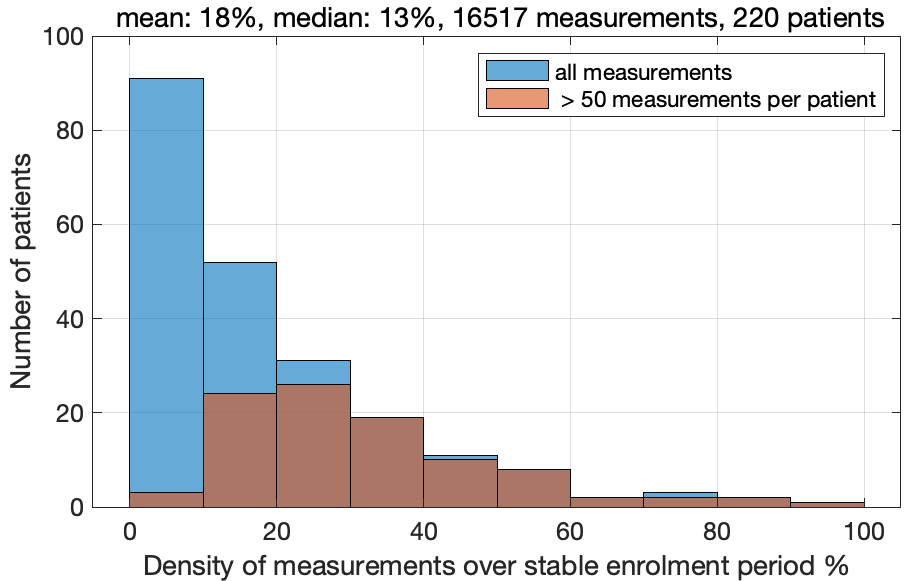
\includegraphics[width=65mm]{images/patientCommitmentFEV1stable.png}
    \caption{Patient commitment to FEV1 recording}
    \label{fig:commitment}
\end{figure}

\subsection{FEV1 variability}
Figure \ref{fig:variability} summarises a set of statistics, for (window size, threshold) pairs describing the residuals' sample, which can be taken as estimates of the variability. All models use over 66\% of patients and over 74\% of all stable measurements available. This strengthens the constraints \textbf{C2} and \textbf{C3}. 

\begin{figure}[!h]
    \centering
    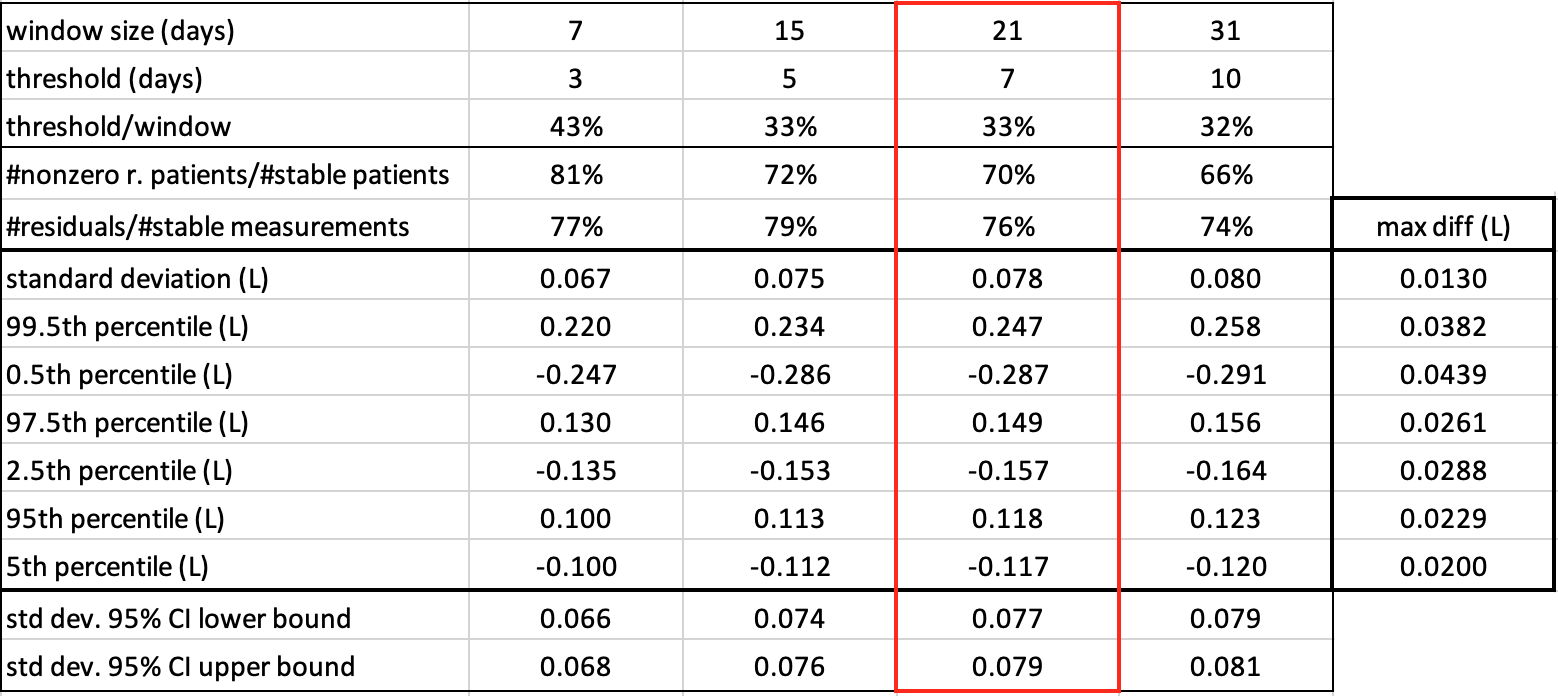
\includegraphics[width=140mm]{images/variabilitytable.png}
    \caption{Model results for different parametrisation}
    \label{fig:variability}
\end{figure}

The sensitivity of the statistics with respect to the choice of the parameters is of the order of 10 mL, which is low since one would expect significant variations in volume to be of the order of 100 mL. Nevertheless, the parametrisation (21,7) is the most conservative to ensure all constraints apply, an example is given in figure \ref{fig:fev1profile}. In fact, with (7,3) and (15,5) the minimum smoothing scale is of 3 and 5 days which is too close to the time-scale of the variations of noise (\textbf{C2}). (31,10) could be the best alternative to (21,7) but 21 days of smoothing window already a conservative choice to ensure that all noise has been removed (\textbf{C1}). 

The 99.5th precentiles is located over three sigma deviations, the 97.5th percentile at 2 sigma, and the 95th percentile at 1.5 sigma. Whereas the 2.5th-97.5th and 5th-95th percentiles ranges are stable, the absolute value of the residuals' are unbalanced nearby the 0.5th percentile compared to the 99.5th percentile. This suggests that the 0.5th-0.95th already contain outliers. The most reasonable statistics to estimate the variability are therefore the 2.5th-97.5th range, or two sigma, leading to a variability of 306 mL, respectively 312 mL. Hence, 310 mL can be set as a clear ground rule for clinicians.

\begin{figure}[!h]
    \centering
    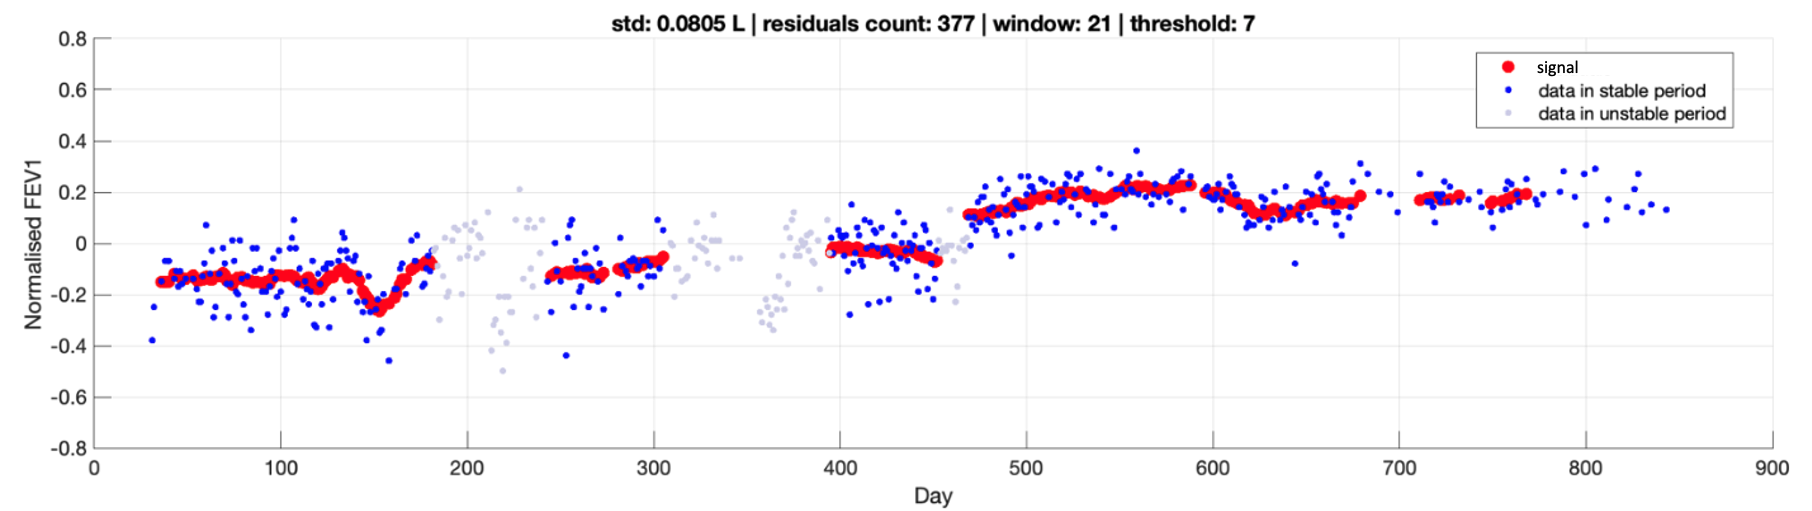
\includegraphics[width=150mm]{images/fevMovingAvg_patient103_w21_t7.png}
    \caption{Patient FEV1 measurements profile with the residuals from the (21,7) moving mean filter}
    \label{fig:fev1profile}
\end{figure}
\subsection{Categorisation of patients' variability}
Based on the standard deviation, the dispersion of the variability among patients is extremely high. The boxplot figure \ref{fig:fev1boxplot} shows that the standard deviation of the patients’ residuals ranges between 46 mL (25th percentile) and 107 mL (75\% percentile), which is more than the double. Defining the variability as two standard deviation, the variability would range in [184; 428] mL. From observations of the FEV1 profiles, the residuals’ standard deviation is an excellent method to segment patients between high, medium and low FEV1 variabilities.

\begin{figure}[!h]
    \centering
    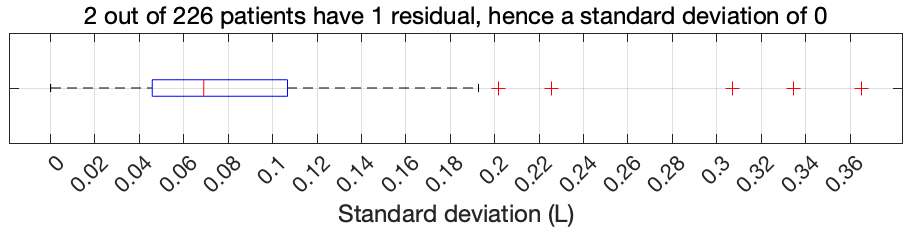
\includegraphics[width=90mm]{images/fev1boxplot.png}
    \caption{Boxplot of the patients' standard deviation in FEV1 measurements}
    \label{fig:fev1boxplot}
\end{figure}

\subsection{Relation with predicted FEV1\%}
Clinically, it would be interesting to know if one could differentiate patients' lung function based on their variability. FEV1 in percent predicted was used to evaluate patients' mean FEV1 on the same reference scale based on their height. However, the Pearson correlation coefficient of 0.129 shows insignificant correlation (p-value = 0.222 \ref{fig:correlation}). 

\begin{figure}[!h]
    \centering
    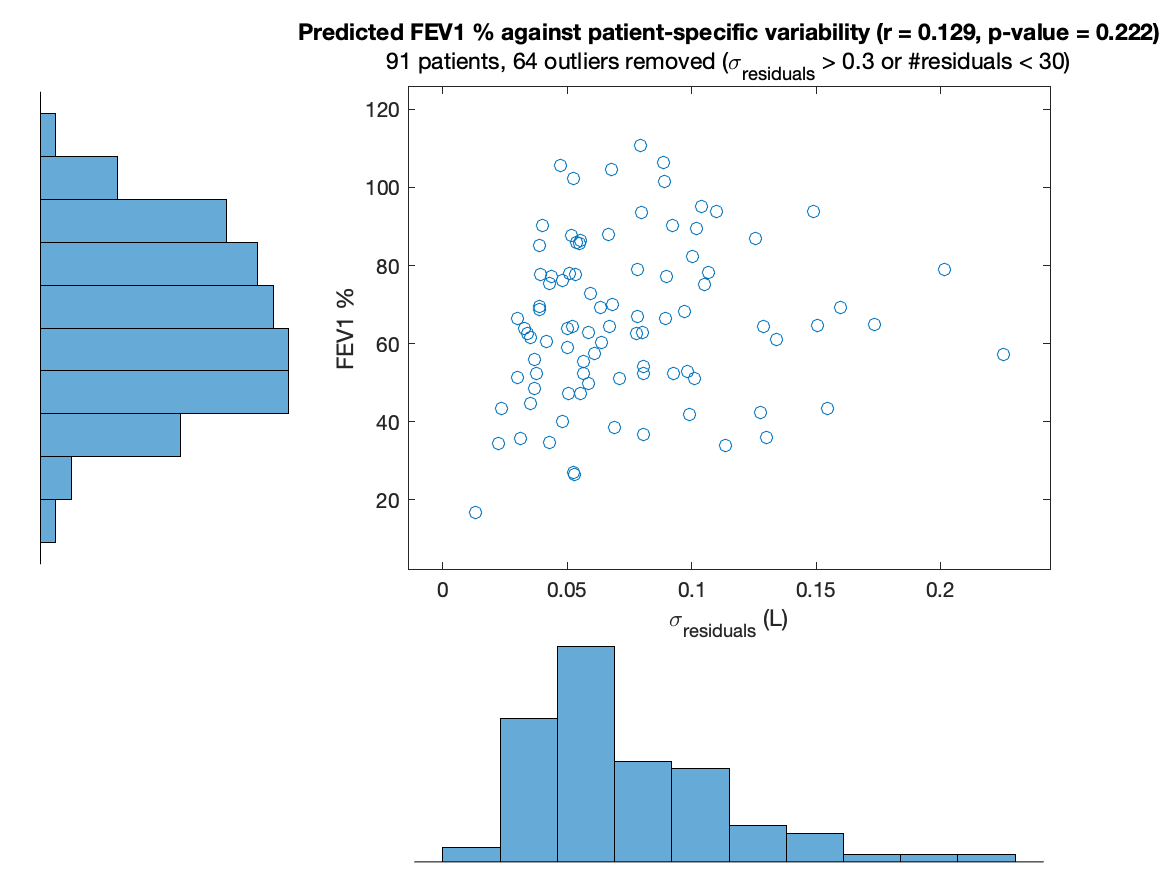
\includegraphics[width=100mm]{images/fevModelBasedAnalysis_variabilityvsFEV1.png}
    \caption{Correlation of variability and lung health}
    \label{fig:correlation}
\end{figure}

\subsection{Effect of CFTR modulator therapies: homoscedasticity test} \label{sec:hptests}
As explained in the introduction, CFTR modulators are transforming life of cystic fibrosis patients. Since 69\% of our participants were prescribed Triple Therapy, and 47\% Symkevi (figure \ref{fig:breathestats}), the data set was deemed sufficiently rich in to analyse the effect of CFTR modulators on the FEV1 variability during stable period. Three homoscedasticity were performed tests on 1) "prior Symkevi" - "during Triple Therapy", 2) "during Symkevi" - "during Triple Therapy", 3) "prior Symkevi" - "during Symkevi", to see if treatments had a significant effect on the reduction in variability. To do that, 5 more patients were removed whose residual's standard deviation were far outlying (> 0.19, figure \ref{fig:fev1boxplot}), in addition to the three from the model parametrisation. 76 patients that were chronologically prescribed Symkevi and then Triple Therapy, were selected. Note that any data after a Triple Therapy stop, this concerned 6 individuals (table \ref{tab:cftrmodulators}), were removed. This data was partitioned into three groups: A) measurements performed prior Symkevi, i.e. no therapy, B) during Symkevi, and C) during Triple Therapy. The Q-Q plot showed that the samples had a Student t-location-scale distribution (figure \ref{fig:qqplot}). Considering samples of over 1000 elements, the few outliers (<20) are indeed negligible. The Student distribution is a two tailed distribution with tails heavier than the normal distribution, and it is very close to the Cauchy distribution for small degrees of freedom and large sample sizes. Since this is the case ($\nu$=\{3;4\}), the best test is therefore the Levene's test with 10\% trimmed mean as defined in \ref{sec:homoscedasticity} as well as an right-tail F-test to maximise robustness. 

\begin{figure}[!h]
    \centering
    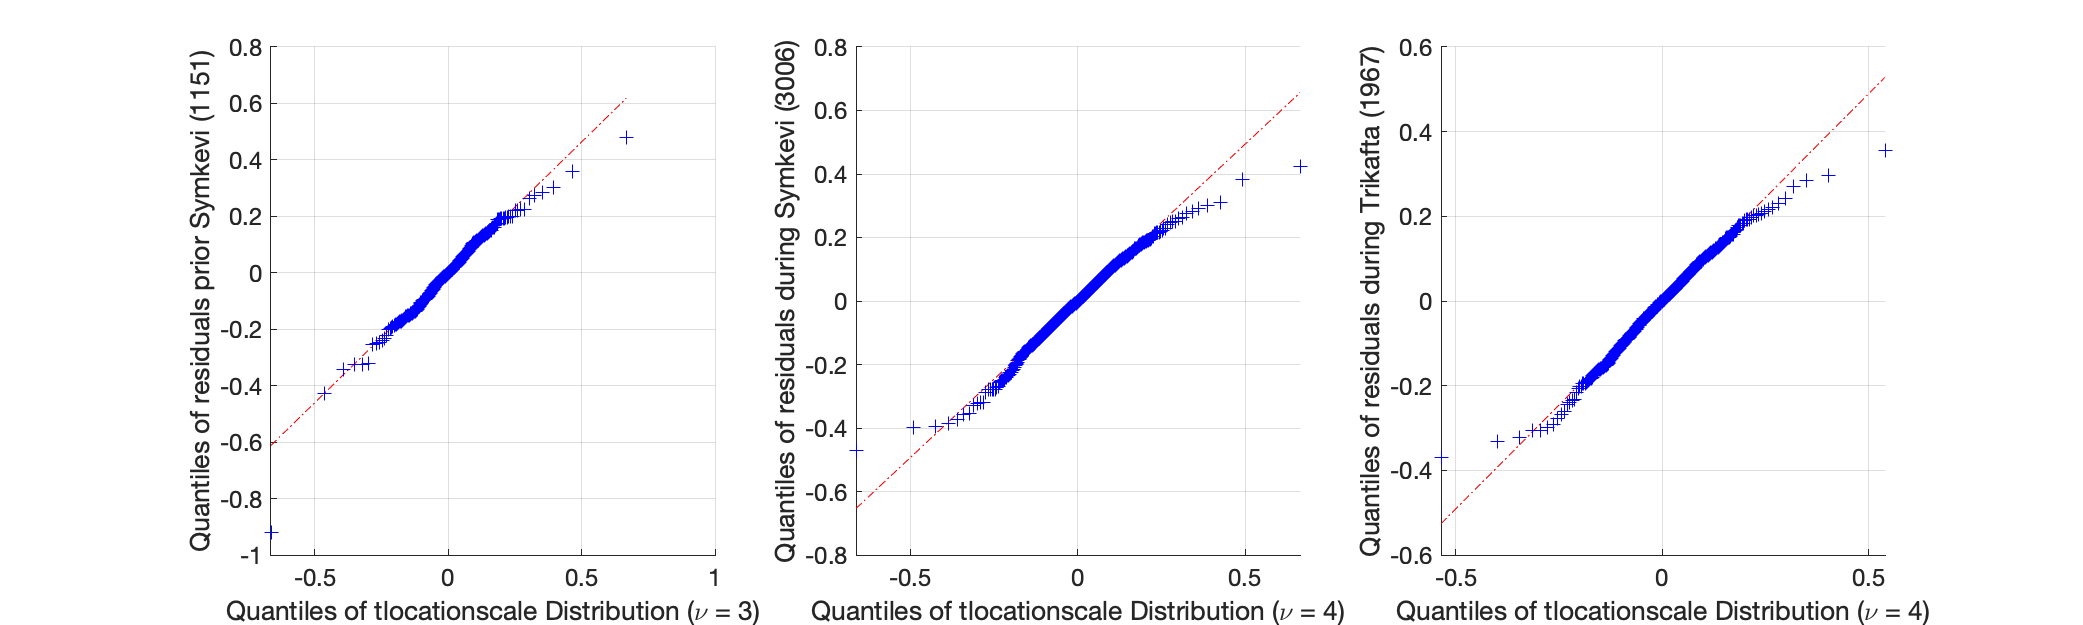
\includegraphics[width=150mm]{images/fevModelBasedAnalysis_qqplot_none_smkv_trpl.png}
    \caption{Q-Q plot of the three groups}
    \label{fig:qqplot}
\end{figure}

The tests 1, 2, 3 summarised on figure \ref{fig:hptests} showed a significant reduction, with below 3\% significance threshold, in the FEV1 variability after the start of Triple Therapy over  Symkevi (7\% reduction in standard deviation) and the start of Triple Therapy over no therapy (17\% reduction in standard deviation). However, the variability reduction was not significant after Symkevi start over no therapy. 

\begin{figure}[!h]
    \centering
    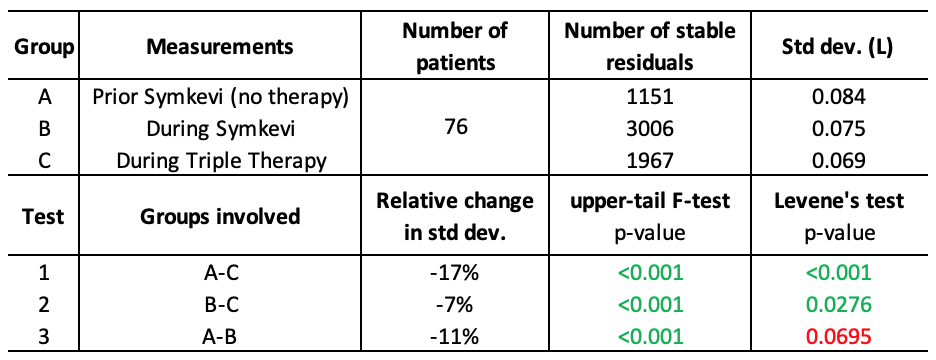
\includegraphics[width=100mm]{images/tests.png}
    \caption{Tests 1, 2, 3 on equality of variance}
    \label{fig:hptests}
\end{figure}

Two additional tests where performed with a similar setting: 4) "anything before Triple Therapy" - "during Triple Therapy", and 5) "anything before Symkevi" (except Triple Therapy) - "during Symkevi". Q-Q plots were extremely close to \ref{fig:qqplot}. Powerful statistical significance for the start of Triple Therapy over any CFTR modulator history (p<0.001) was obtained, but not for Symkevi against prior therapies (figure \ref{fig:hptests2}.

\begin{figure}[!h]
    \centering
    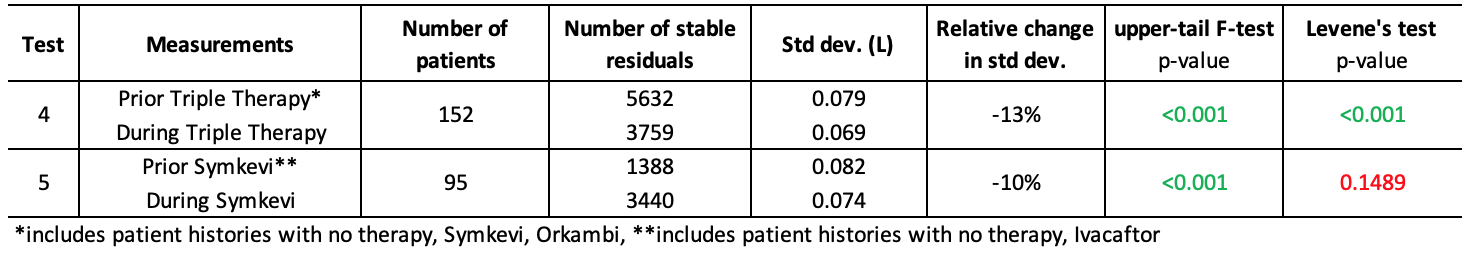
\includegraphics[width=150mm]{images/hptests2.png}
    \caption{Tests 4, 5 on equality of variance}
    \label{fig:hptests2}
\end{figure}


\section{Discussion}
A model was created to estimate the FEV1 measurements variability based on the residual's of a bi-parameter moving mean filter. Based on 150 patients and 12550 measurements, the variability of FEV1 measurements was estimated to 310 mL, using the span of the 2.5, 97.5th percentile in figure \ref{fig:variability}. This results is more conservative than for the standard deviation, the gold standard for measuring variability. Also, it verifies the work from Cooper et al., 1990 who estimated it to 260 mL, using the 95th percentile (this would give 230 mL in this study \ref{fig:variability}), with a much smaller data set of 28 patients and 9 measurements each \cite{cooper_1990}.

However, \textbf{the variability is extremely diverse among patients}, with a median at 276 mL and large interquartile range deviations of -92 mL (-33\%) and +152 mL (+55\%). Consequently, any precise study of FEV1 signal should not use a global approximation for the FEV1 variability to distinguish signal from noise, but rather a much more precise patient-specific value, which can be selected as the patient's standard deviation of the residuals. Additionally, this variability could be explained with predicted FEV1\% (Pearson correlation coefficient r=0.129). 

Eventually, it was demonstrated powerfully and robustly that \textbf{the start of Triple Therapy led to significant mitigation of the variability} in FEV1 over \textit{any} previous CFTR modulator therapy history available, with six hyptohesis tests (with p<0.001 for 5 of them). Also important, statistical significance for reduction in FEV1 variability for the start of Symkevi over any previous CFTR modulator therapy history available was not shown.

\subsubsection{Model limitations}
After removing unstable measures, the dataset can still contain day-to-day signal variations because 1) some CFTR modulator events may not have been recorded by hospitals, and 2) stable periods of FEV1 measurements can contain unstable measurements.  Nonlinearities in the measurement device output can modify the scale of signal and noise for each measurement, thus perturbing the results. The extent to those limitations are unknown and standard for a clinical study involving manually reported values and measurements.

\begin{appendices}

\chapter{Project Breathe's patient demographics, treatments and measures list} \label{sec:appendixbreathe}
The figures \ref{fig:breathestats}, \ref{fig:enrolmenttime}, \ref{fig:nintr}, were drawn for study patients enrolled from Royal Papworth and Cardiff Hospitals on the period from 30.12.2019 to 15.06.2021)

\begin{figure}[!htb]
   \begin{minipage}{0.48\textwidth}
     \caption{Patients demographics}
    \centering
    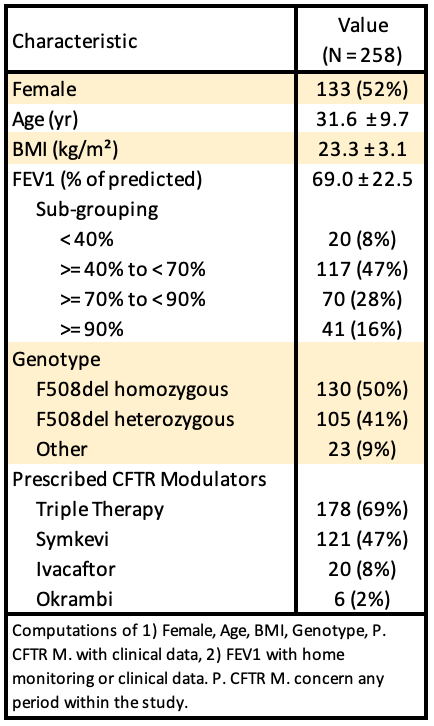
\includegraphics[width=60mm]{images/breathestats.png}
    \label{fig:breathestats}
   \end{minipage}\hfill
   \begin{minipage}{0.48\textwidth}
   
     \caption{Participants' enrolment time}
    \centering
    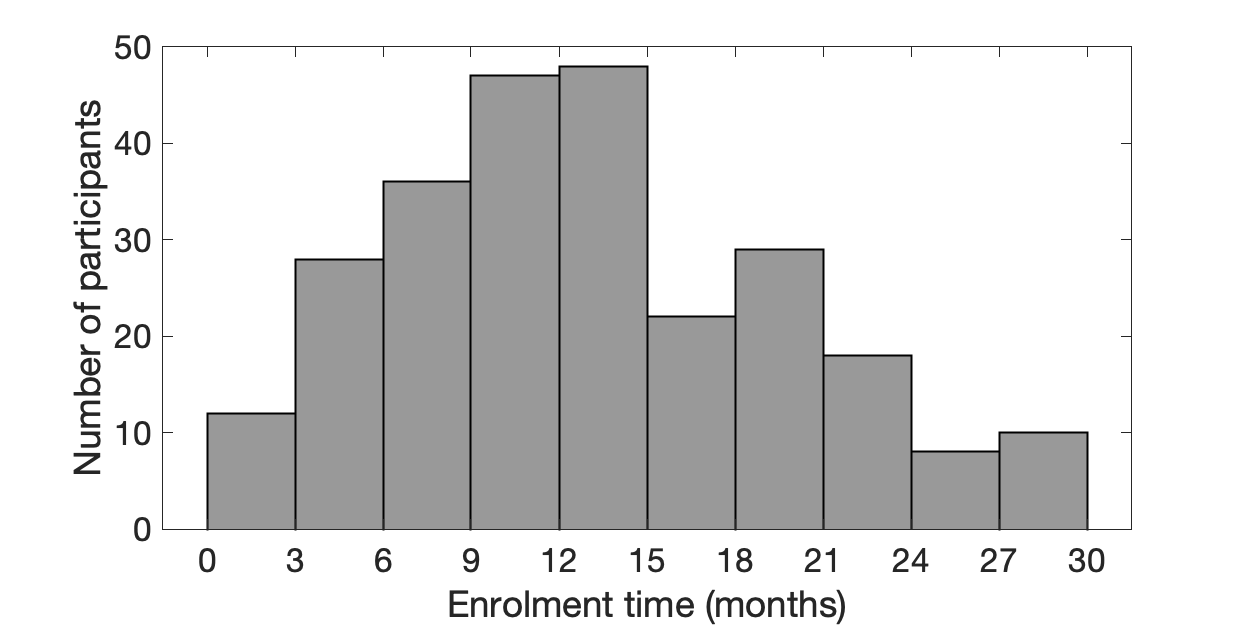
\includegraphics[width=80mm]{images/Patient_enrolment_time_from30-Dec-2019_to15-Jun-2021.png}
    \label{fig:enrolmenttime}
    
    \caption{Number of interventions per participants}
    \centering
    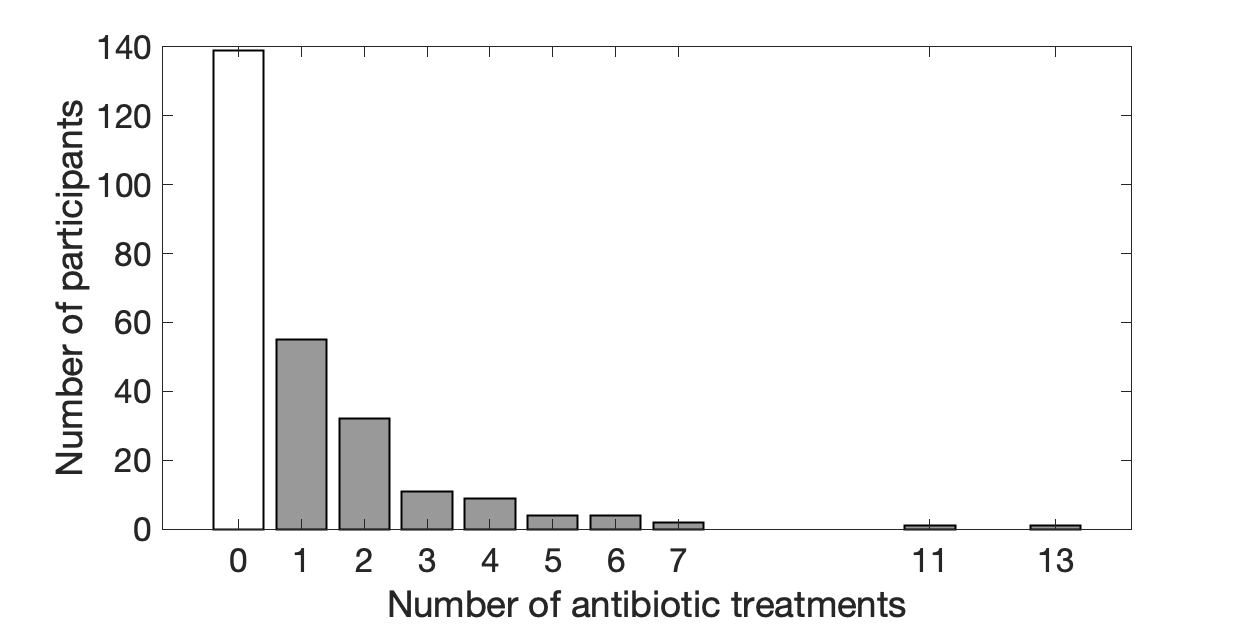
\includegraphics[width=80mm]{images/bar_intrperpatient_before_filter.png}
    \label{fig:nintr}
    
   \end{minipage}
\end{figure}

    
    \begin{table}[]
        \centering
        \begin{tabular}{c|c}
        \hline
             \textbf{CFTR modulator history} & \textbf{Number of participants} \\
             \hline
             Triple Therapy & 85 \\
             Symkevi - Triple Therapy & 78 \\
             No therapy & 35 \\
             Symkevi & 28 \\
             Ivacaftor & 16 \\
             Ivacaftor - Triple Therapy & 3 \\
             Orkambi - Triple Therapy & 3 \\
             Triple Therapy - Symkevi & 3 \\
             Triple Therapy - Therapy stopped & 2 \\
             Ivacaftor - Symkevi & 1 \\
             Symkevi - Triple Therapy - Symkevi & 1 \\
             \hline
        \end{tabular}
        \caption{Participants' CFTR modulators therapy history status on 15.06.2021, chronologically from left to right. }
        \label{tab:cftrmodulators}
    \end{table}

\begin{table}
\begin{tabular}{l|l|l} 

\hline

\textbf{Measure} & \textbf{Description}  & \textbf{Recording method}  \\ 
\hline
Wellness & Answering "How are you feeling today?" & 
\begin{tabular}[c]{@{}l@{}} 1 (Very Unwell) \\ to 10 (Great) \end{tabular}   \\
Cough & Answering 'How is your cough today?"  & 
\begin{tabular}[c]{@{}l@{}} 1 (No Cough) \\ to 10 (Chronic) \end{tabular}   
  \\
FEF2575 & 
\begin{tabular}[c]{@{}l@{}}Mean forced expiratory flow between the 25\% \\and the 75\% of the total volume exhaled\end{tabular}   
\\
FEV075         & Forced expiratory volume in 0.75"   & Spirometer \\
FEV1DivFEV6    & Division of FEV1 by FEV6  & Spirometer\\
FEV1           & Forced expiratory volume in 1"  & Spirometer \\
FEV6           & Forced expiratory volume in 6"  & Spirometer \\
PulseRate      & Heart rate recorded & HR sensor  \\
RestingHR      & Resting heart rate  & Fitbit/AppleHealth \\
O2Saturation   & O2 saturation level & Oximeter \\
Temperature    & Temperature in °C & Themometer   \\
Weight         & Weight in kg & Scale   \\
Calorie        & Calories  & Fitbit/AppleHealth \\
MinsAsleep     & Mintues spent "awake" while sleeping   & Fitbit/AppleHealth \\
MinsAwake      & Minutes spent actually sleeping  & Fitbit/AppleHealth \\
HasColdOrFlu   & Reacting to "I've got a cold or flu" & True/False slider \\
HasHayFever    & Reacting to "I've got hay fever" & True/False slider  \\
HasHaemoptysis & Reacting to "Haemoptysis" & True/False slider \\
\hline

\end{tabular}
\caption{Recorded measures}
\end{table} \label{tab:measures}

\chapter{Example of patient longitudinal data}

    \begin{figure}[!h]
    \caption{Clinical measurements data}
    \centering
    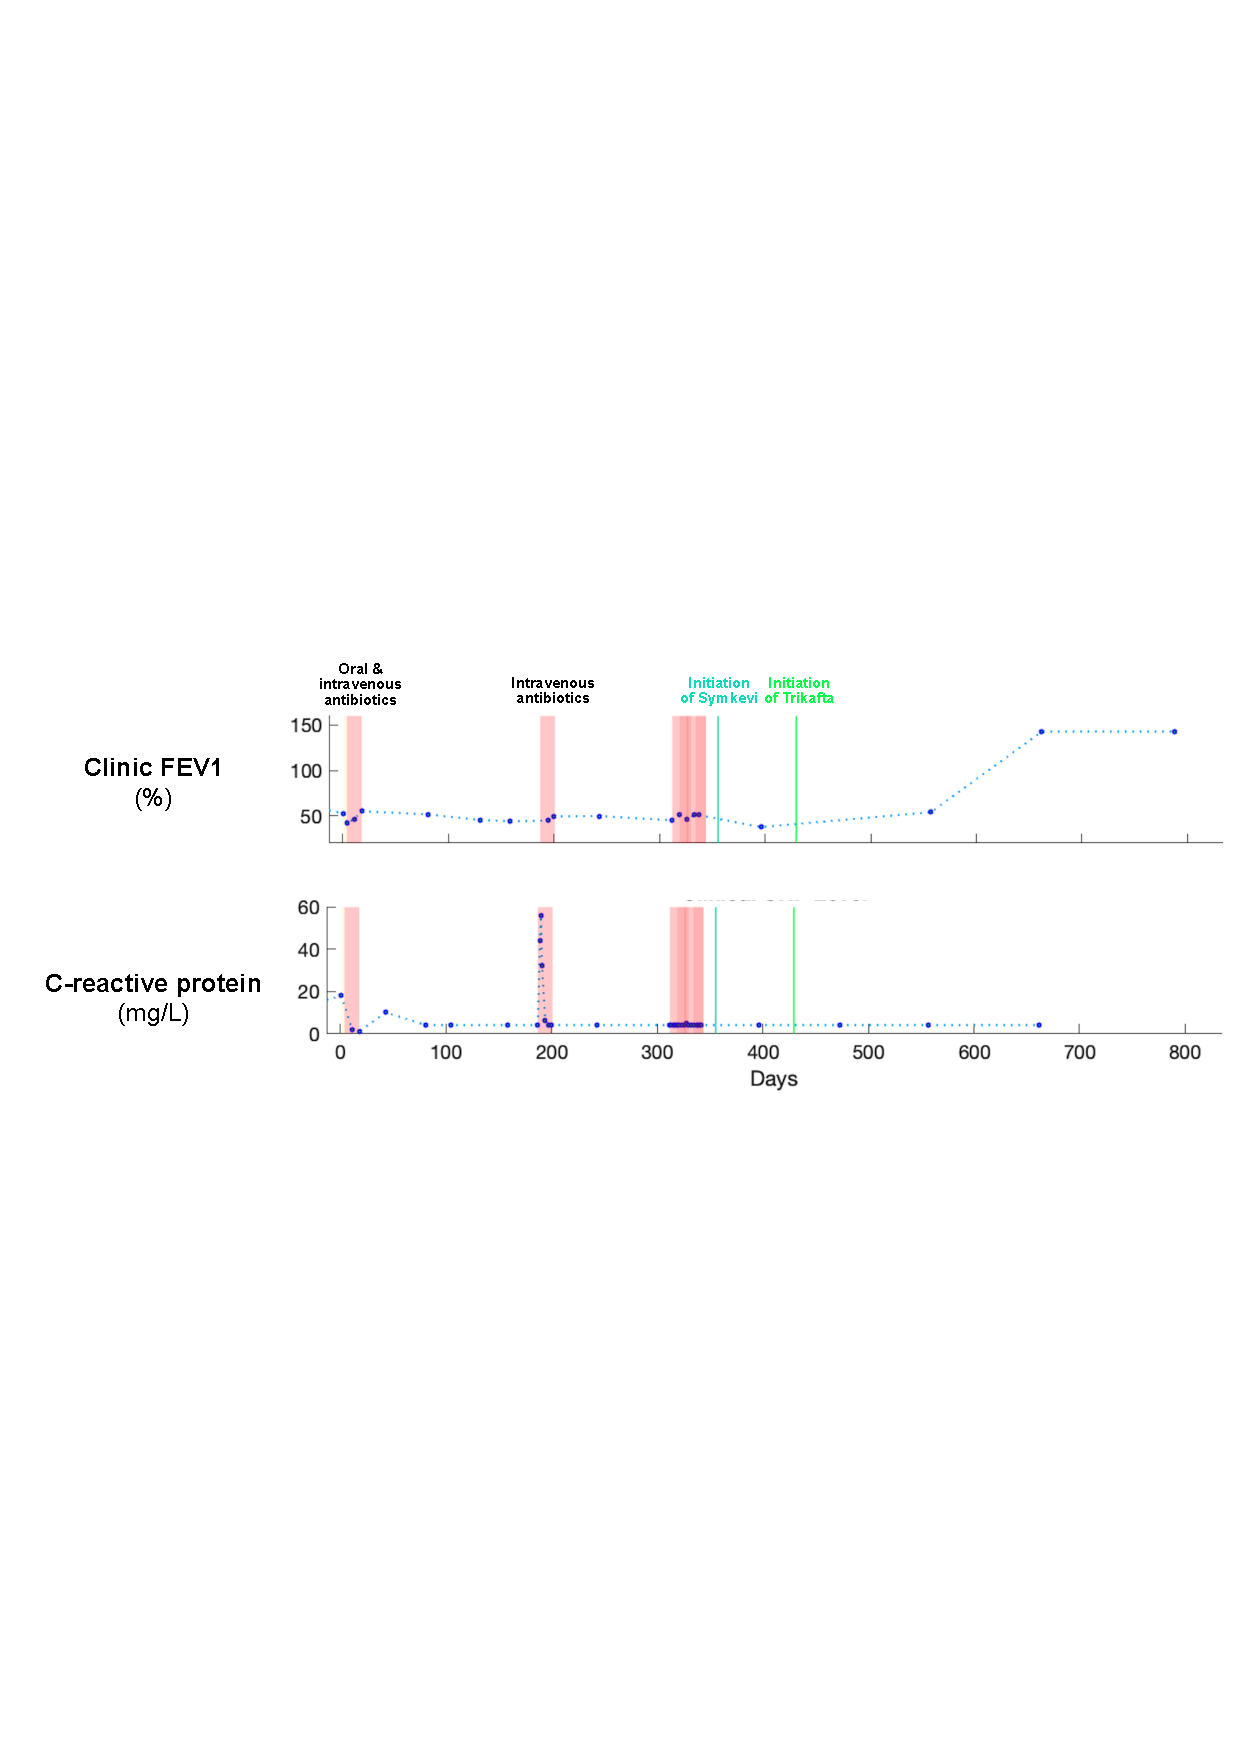
\includegraphics[width=96mm]{images/clinicdata.pdf}
    \label{fig:clinic}
    \end{figure}
    
    \begin{figure}[!h]
    \caption{Home measurements data, with patient measures' mean and standard deviations}
    \centering
    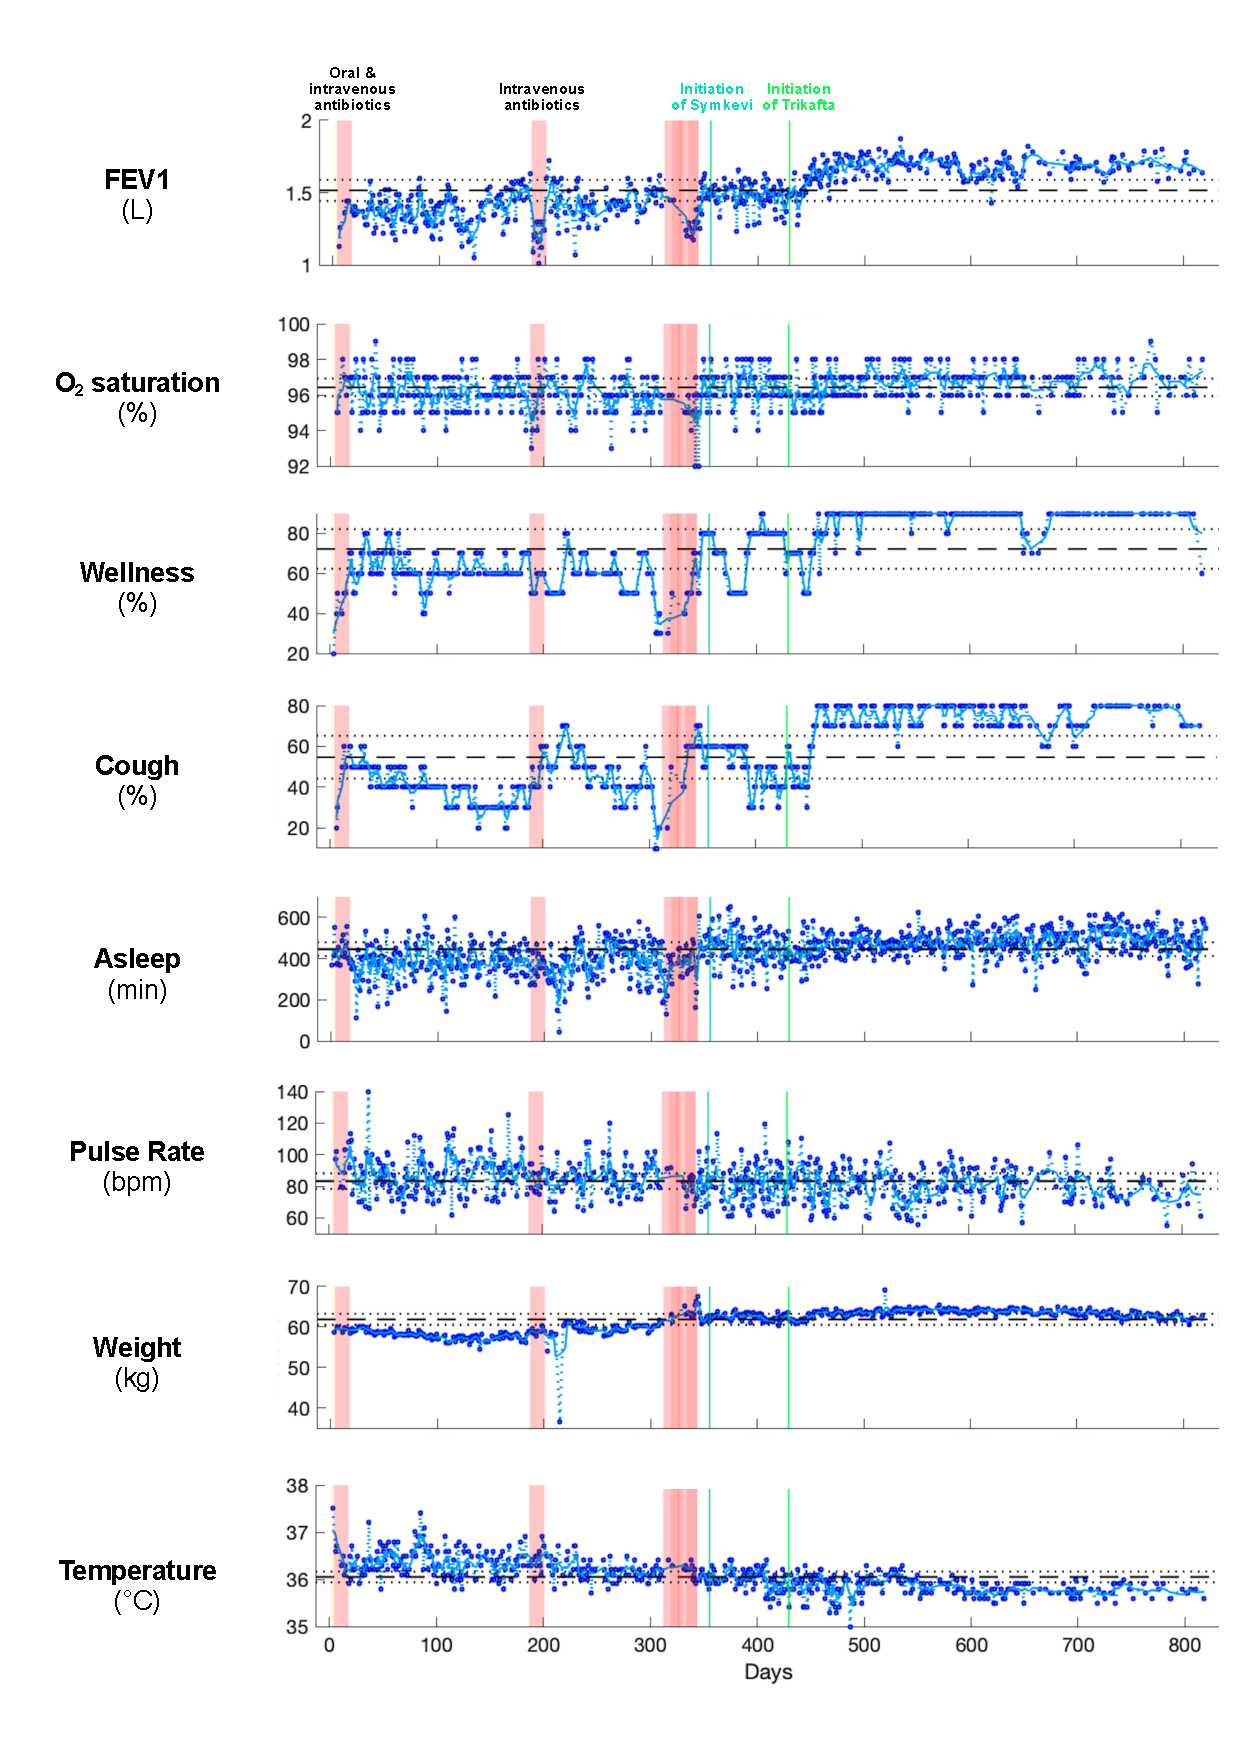
\includegraphics[width=96mm]{images/homedata.pdf}
    \label{fig:home}
    \end{figure}

\chapter{Data quality check}
A rigorous process of data quality assurance was conducted on both the clinical meta-data and the home measurement data. A summary of the specific cases and related actions is detailed in Figure \ref{fig:dataqualitycheck}.

For the clinical data, potentially anomalous values for FEV1, age, weight, height, CRP were identified, as well as inconsistencies between the different types of meta-data – for example a hospital admission without an antibiotic treatment. Whilst not definitively highlighting a data problem, such items were sent back to each of the centres for review and any necessary corrections were applied to the data set.

For the home measurement data, a similar process to identify potentially anomalous values was applied, resulting in a small number of suspect data points being excluded. In addition, data uploads before and after midnight were analysed to ensure they were applied to the correct date. Finally, there were a number of data records with more than one recording for a given measure on a given day – which could have indicated a problem with an automated upload to the servers, or an intentional correction to a previously entered number, or genuinely taking multiple readings per day. A detailed analysis was performed, and corrective actions were taken where possible.

    \begin{figure}[!h]
    \caption{Data quality check and actions performed}
    \centering
    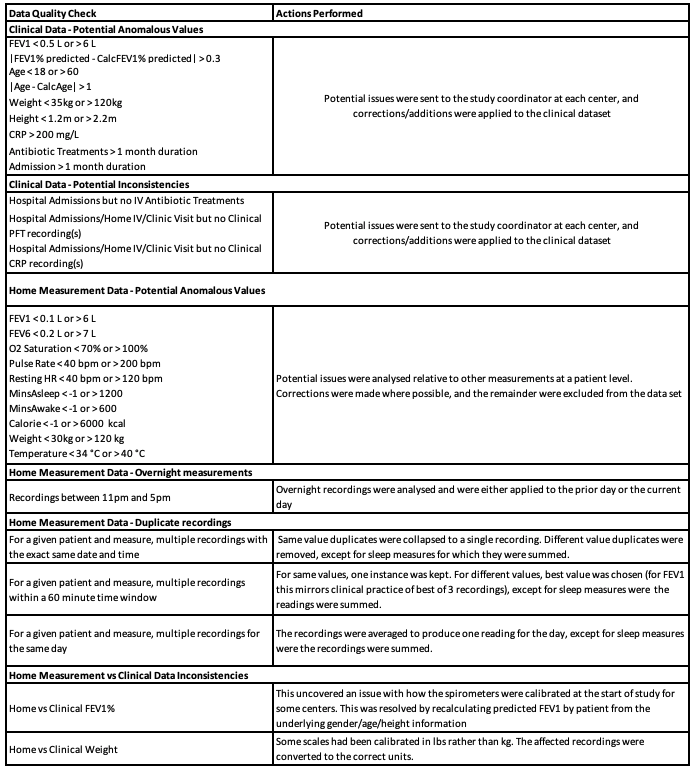
\includegraphics[width=150mm]{images/dataqualitycheck.png}
    \label{fig:dataqualitycheck}
    \end{figure}

\chapter{Examples of three participants interventions profiles} \label{sec:appendixint}
Figures \ref{fig:intrfull}, \ref{fig:intrivpbo} and \ref{fig:intrdecline} respectively show a full recovery from 14 days IV treatment, a successful recovery from 20 days of IV treatment preceded by oral treatment (IVPBO), an unsuccessful recovery characterised by a continuous decline despite treatment. The data records used by the probabilistic inference algorithm ranges from day 0 to day 20 from this graph. The stable baseline is defined as the mean of the upper 75\% of measurements from 35 to 25 days prior to treatment. Note that 1) on the profiles, the temperature, and pulse rate are inverted, and 2) an increase in wellness and cough (displayed in percentage) indicate a diminution of wellness, respectively cough.
    
    \begin{figure}[!h]
    \caption{Successful recovery (back to stable baseline and stabilisation for most measures) delayed due to stacked antibiotics: IV preceded by oral (IVPBO)}
    \centering
    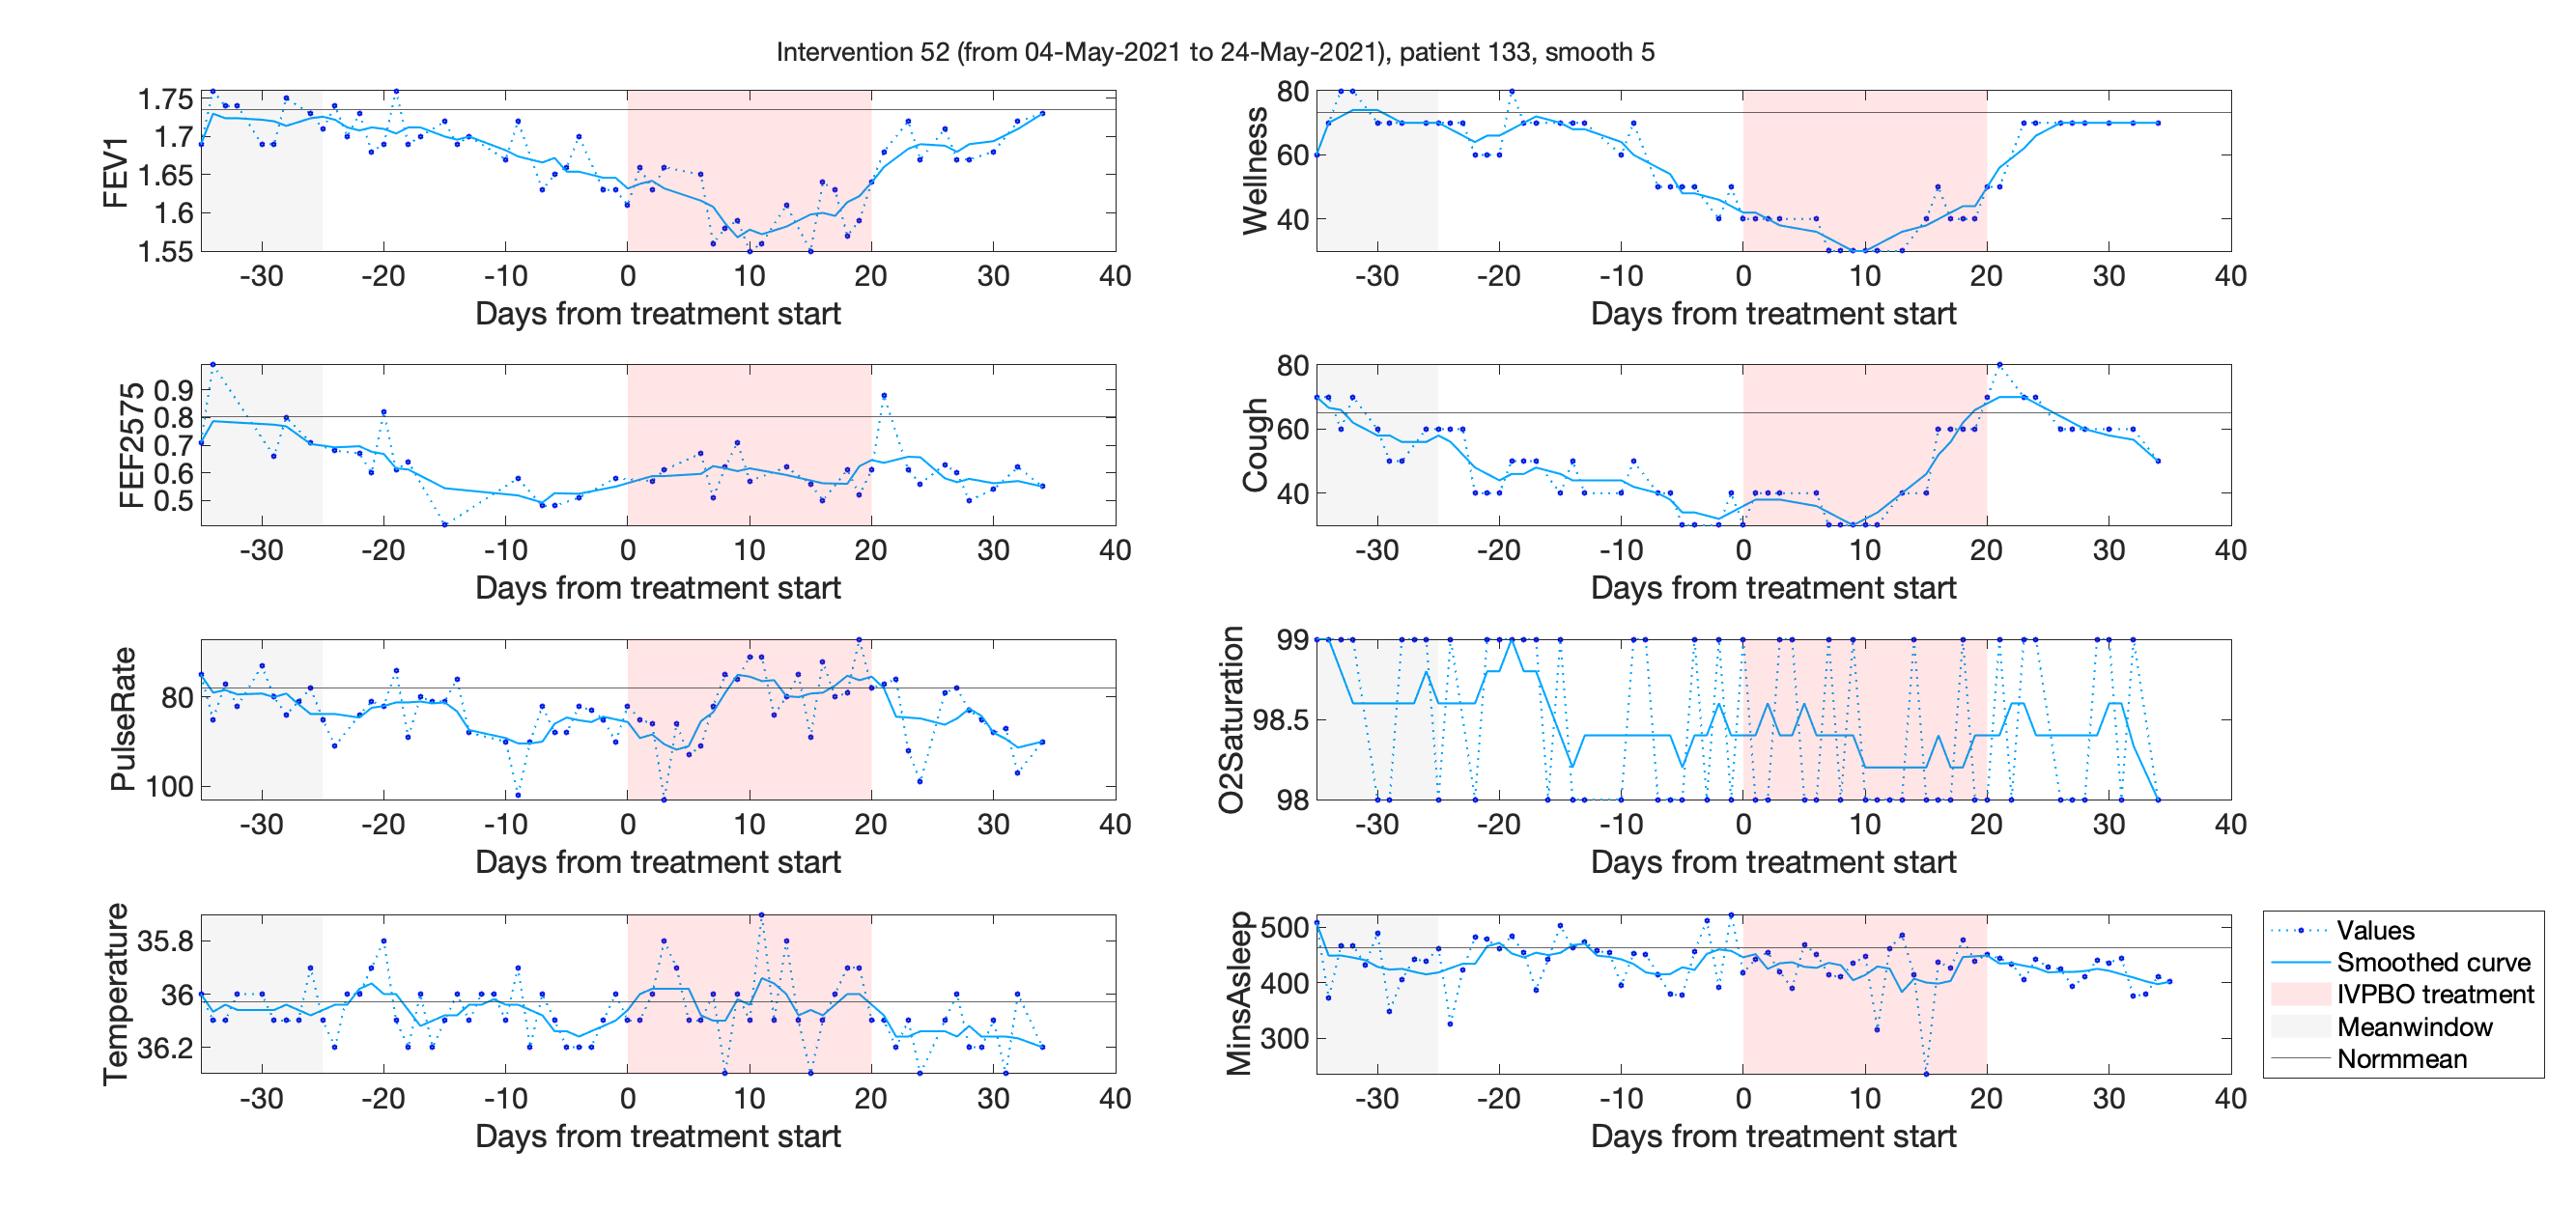
\includegraphics[width=150mm]{images/Intervention52_ID133.png}
    \label{fig:intrivpbo}
    \end{figure}
    
    \begin{figure}[!h]
    \caption{Full recovery (back to stable baseline with overshoot) followed by decline from IV treatment}
    \centering
    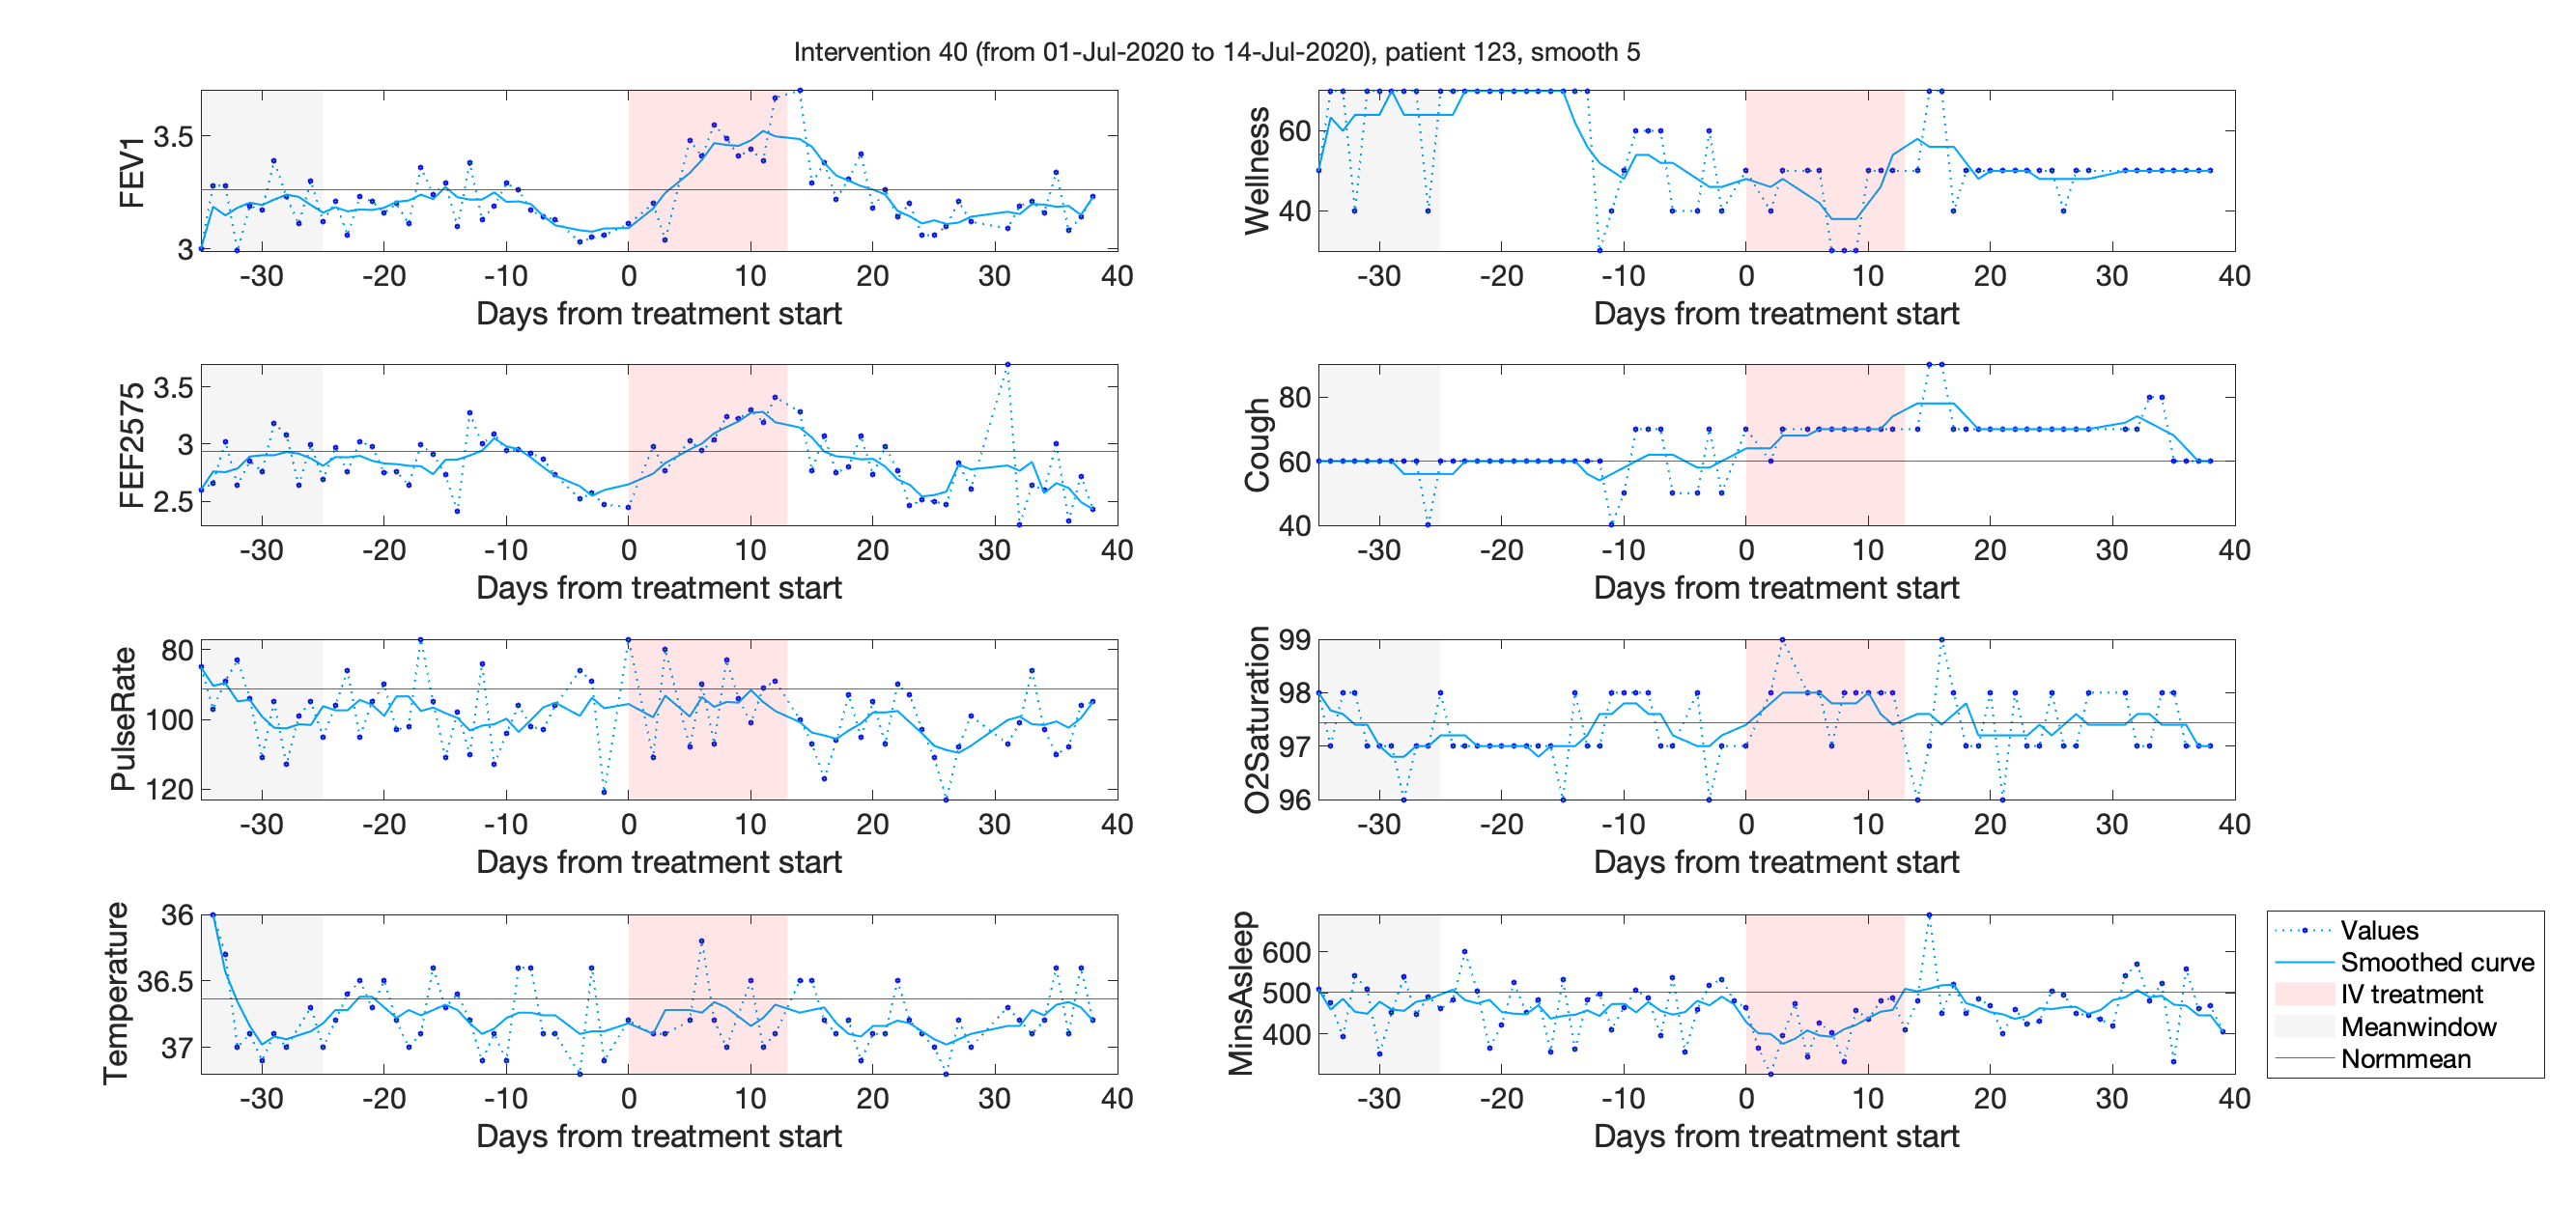
\includegraphics[width=150mm]{images/Intervention40_ID123.png}
    \label{fig:intrfull}
    \end{figure}
    
    \begin{figure}[!h]
    \caption{Continuous decline despite oral antibiotic treatment}
    \centering
    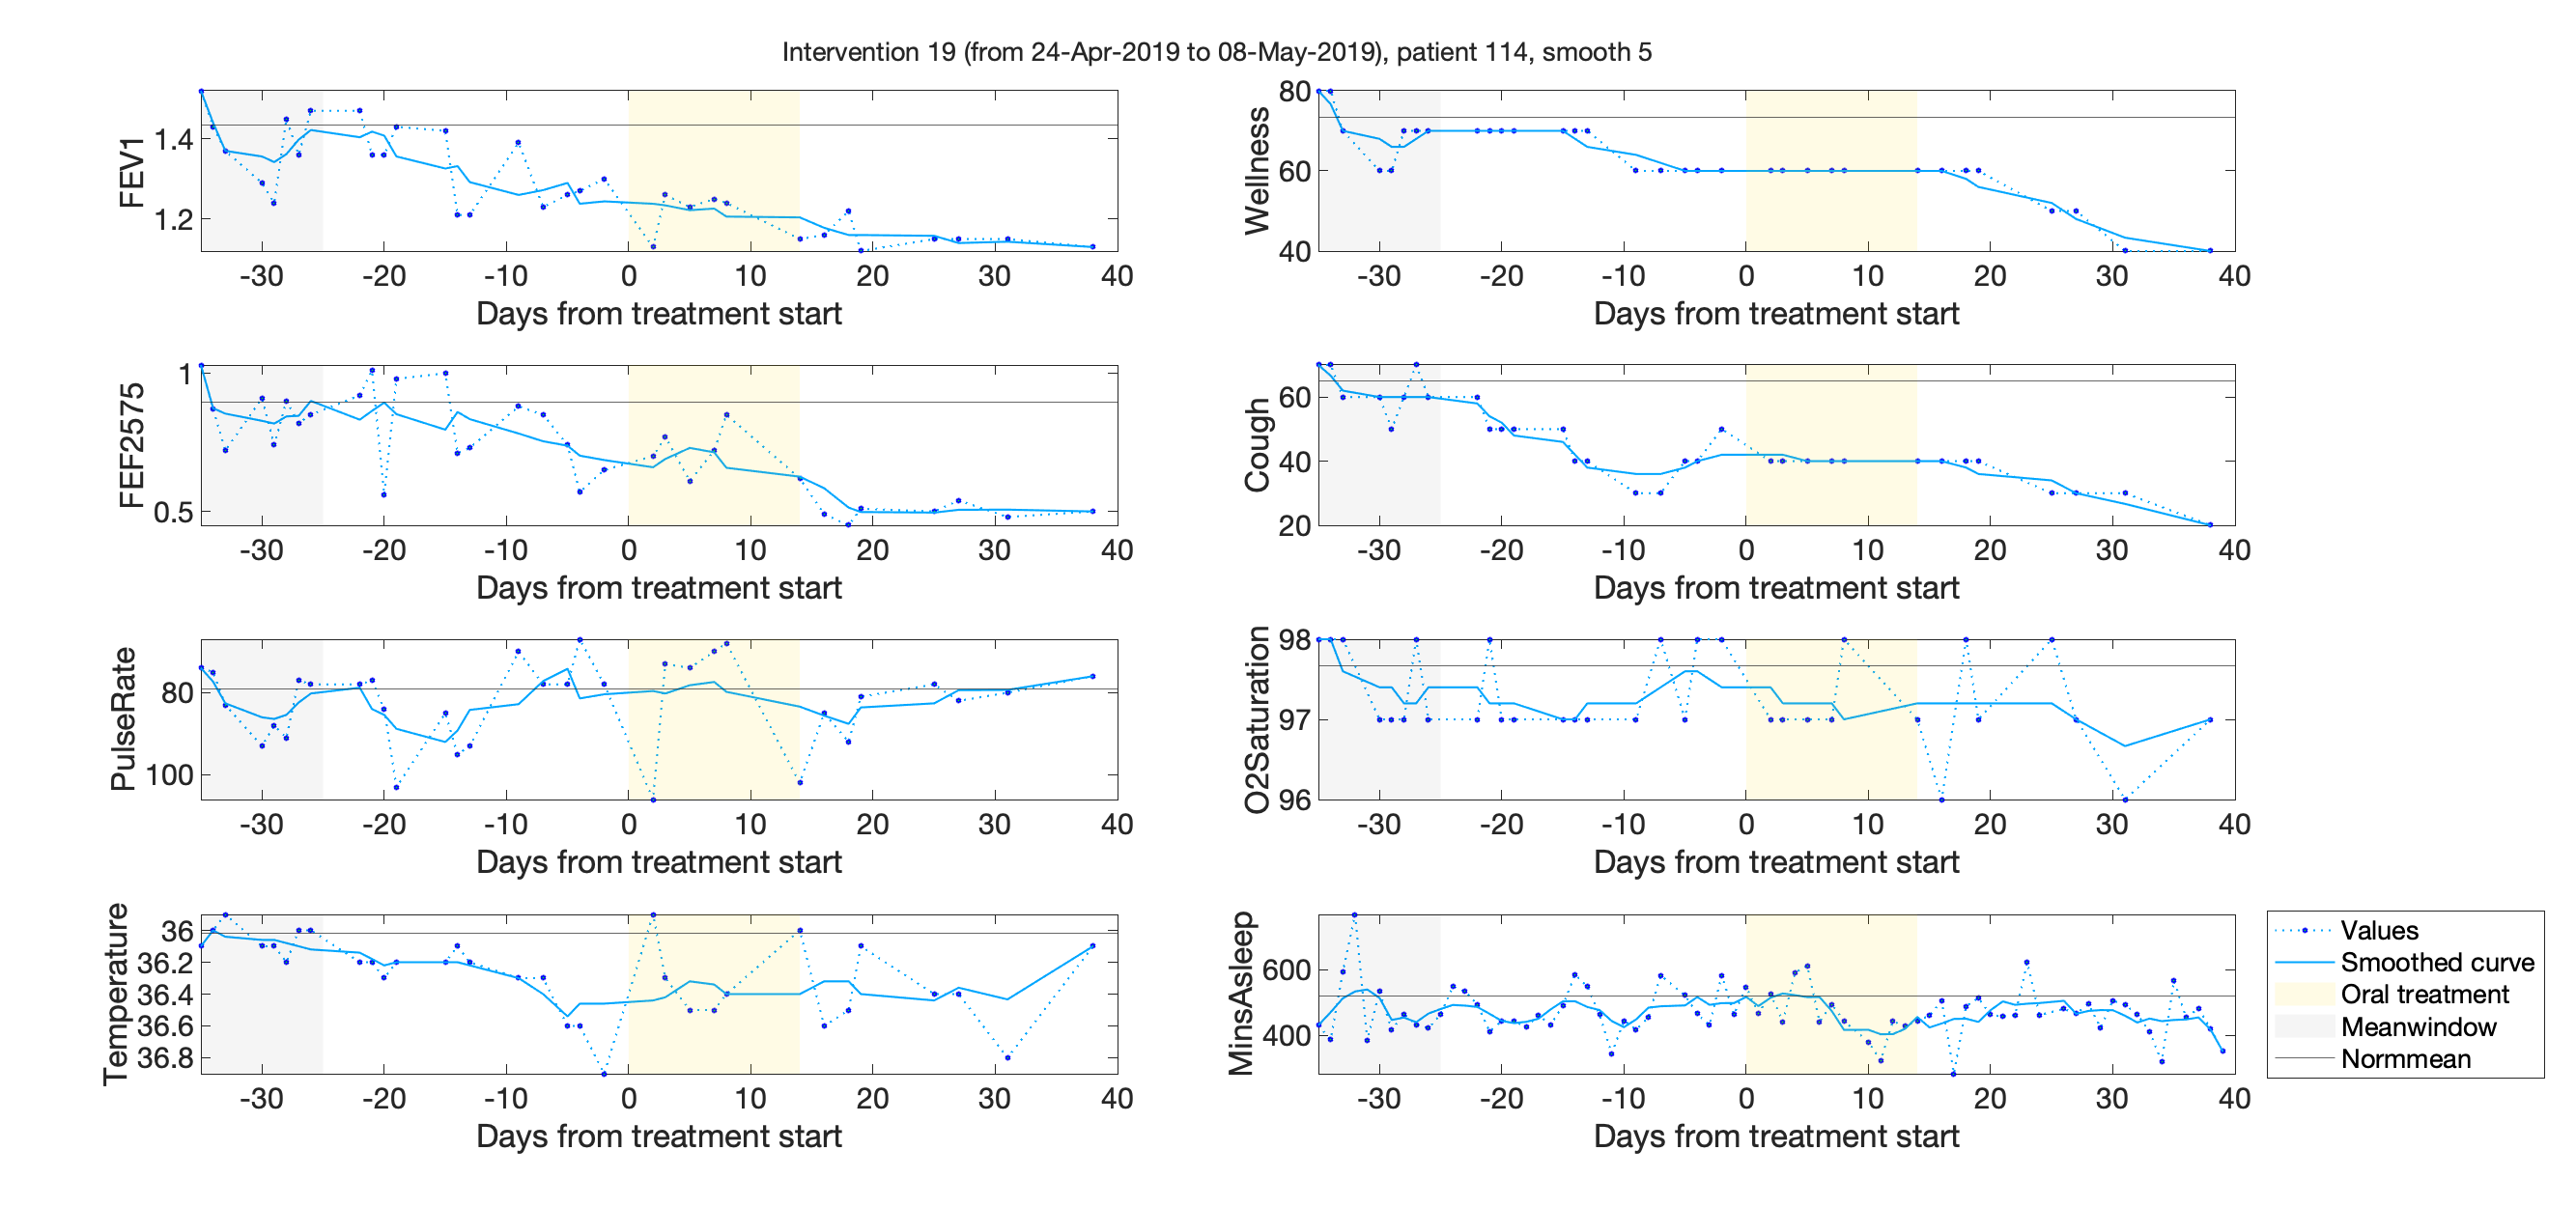
\includegraphics[width=150mm]{images/Intervention19_ID114.png}
    \label{fig:intrdecline}
    \end{figure}
    



    
\end{appendices}
\cleardoublepage
\phantomsection
\setcitestyle{square}
\bibliographystyle{abbrv}
\bibliography{tail/bibliography}
\addcontentsline{toc}{chapter}{Bibliography}


\end{document}